% Exemplo de dissertação do INF-UFG com texto em portugues formatado com LaTeX
\documentclass[dissertacao]{inf-ufg}
\usepackage{amsmath} 
\usepackage{pdfpages}
% Opções da classe inf-ufg (ao usar mais de uma, separe por vírgulas)
%   [tese]         -> Tese de doutorado.
%   [dissertacao]  -> Dissertação de mestrado (padrão).
%   [monografia]   -> Monografia de especialização.
%   [relatorio]    -> Relatório final de graduação.
%   [abnt]         -> Usa o estilo "abnt-alf" de citação bibliográfica.
%   [nocolorlinks] -> Os links de navegação no texto ficam na cor preta.
%                     Use esta opção para gerar o arquivo para impressão
%                     da versão final do seu texto!!!

%----------------------------------------------------- INICIO DO DOCUMENTO %
\begin{document}
%\selectlanguage{portuguese}

%------------------------------------------ AUTOR, TÍTULO E DATA DE DEFESA %
\autor{Werikcyano Lima Guimarães} % (José da Silva)
\autorR{Guimarães Lima, Werikcyano} % (da Silva, José)

\titulo{Aquisição Progressiva de Habilidades por meio de Curriculum Learning para Futebol de Robôs Multiagente}
%\subtitulo{\textless Subtítulo do Trabalho\textgreater}

\cidade{Goiânia} % Nome da cidade em foi desenvolvido o trabalho
\dia{06} %
\mes{Janeiro} % Data da apresentação/defesa do trabalho
\ano{2025} % Formato numérico: \dia{01}, \mes{01} e \ano{2009}

%-------------------------------------------------------------- ORIENTADOR %
\orientadora{ Dra. Telma Woerle de Lima Soares}
%\orientadoraR{\textless Nome Reverso do Orientador\textgreater}
% Use os comandos a seguir se for Orientadora e nao Orientador.
%\orientadora{\textless Nome da Orientadora\textgreater}
%\orientadoraR{\textless Nome Reverso da Orientadora\textgreater}

%\coorientador{\textless Nome do Co-orientador\textgreater}
%\coorientadorR{\textless Nome Reverso do Co-orientador\textgreater}
% Use os comandos a seguir se for Co-orientadora e nao Coorientador.
%\coorientadora{\textless Nome da Co-orientadora\textgreater}
%\coorientadoraR{\textless Nome Reverso da Co-orientadora\textgreater}

%-------------------------------------------------- INSTITUIÇÃO E PROGRAMA %
\universidade{Universidade Federal de Goiás} % {Universidade Federal de Goiás}
\uni{UFG}         % UFG
\unidade{Instituto de Informática} %Instituto de Informática
%\departamento{\textless Nome do Departamento\textgreater} %Unidades com mais de um depto.

%\universidadeco{\textless Nome da Universidade do Co-orientador\textgreater}
%\unico{\textless Sigla da Universidade do Co-orientador\textgreater}
%\unidadeco{\textless Nome da Unidade Acadêmica do Co-orientador\textgreater}

\programa{Ciência da Computação} % Computação
\concentracao{Ciência da Computação}

%-------------------------------------------------- ELEMENTOS PRÉ-TEXTUAIS %
\capa    % Gera o modelo da capa externa do trabalho
%\publica % Gera a autorização para publicação em formato eletrônico
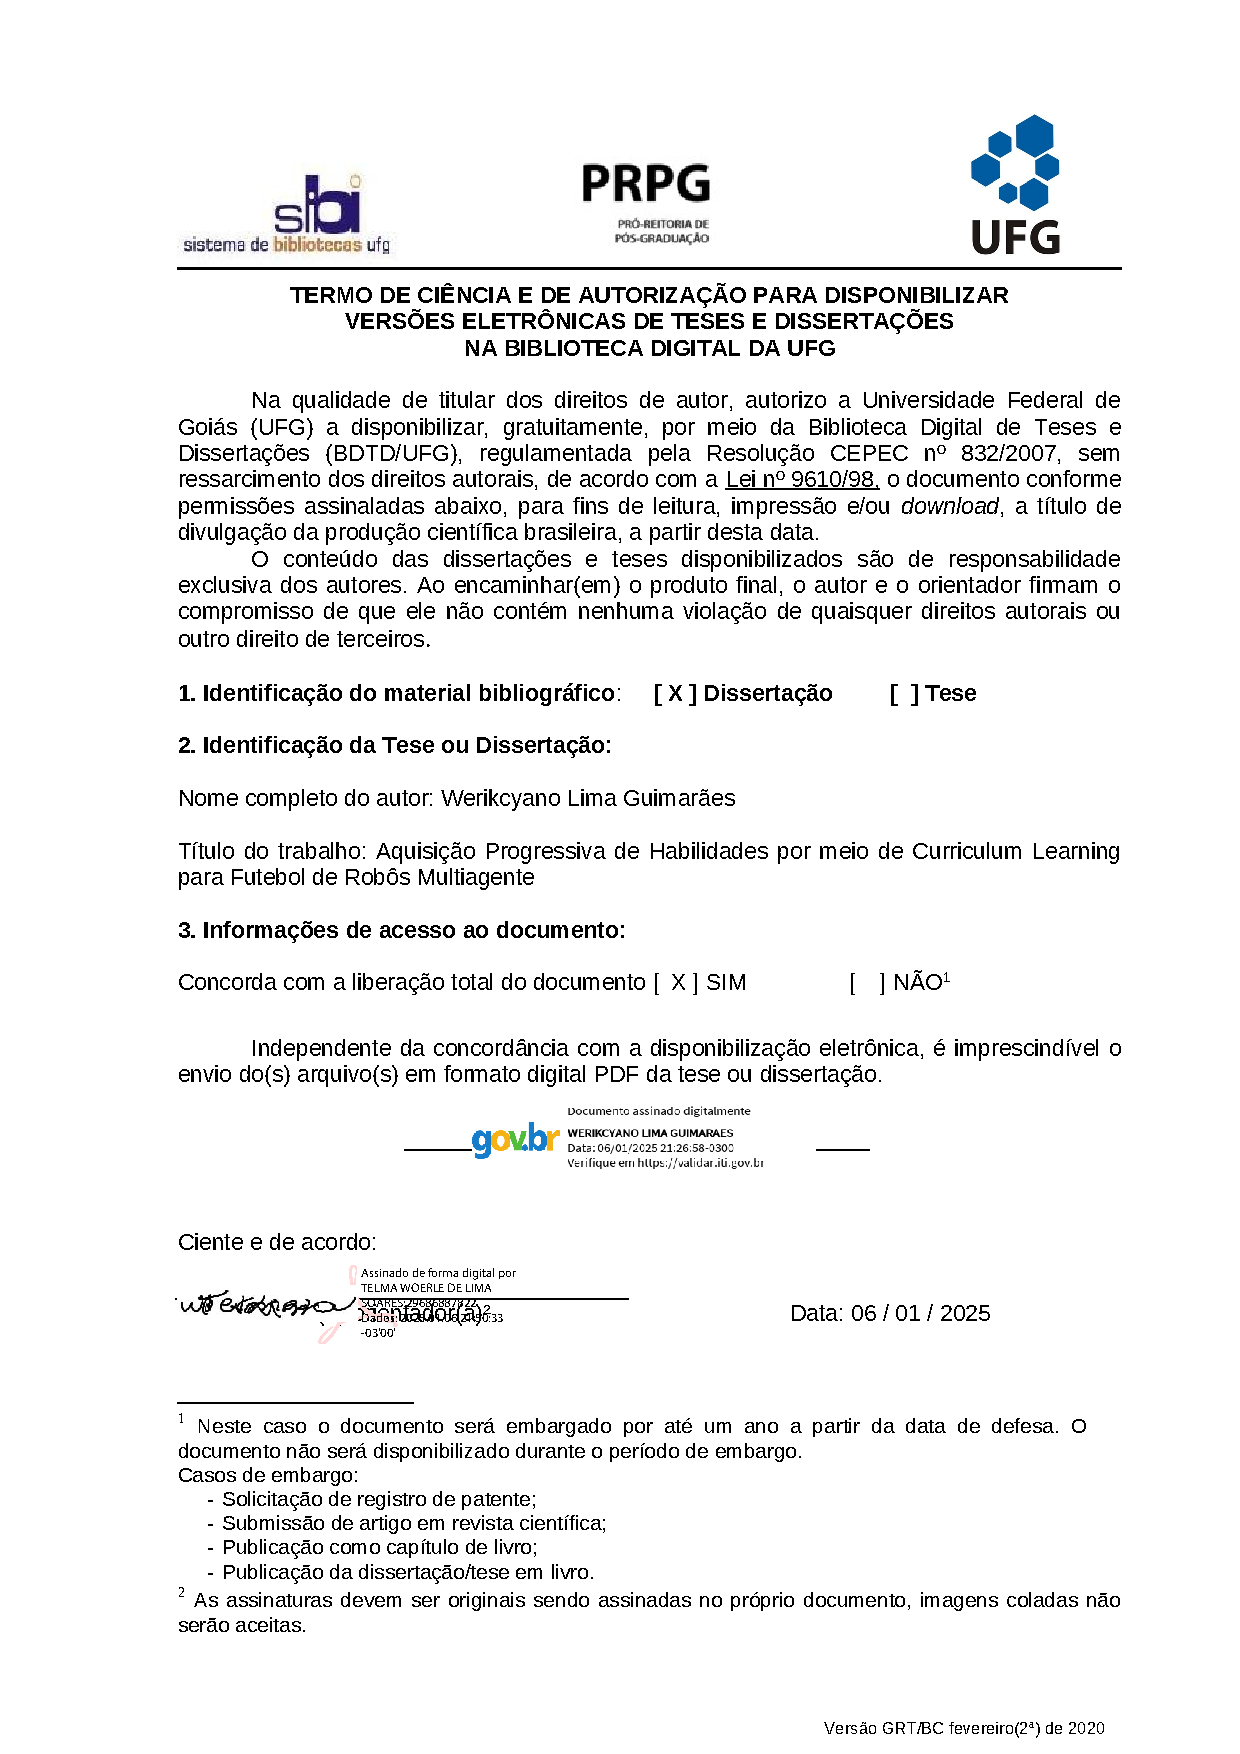
\includepdf[pages=-, scale=1, angle=0,  offset=0 -50]{pre/TECA_preenchido_assinado.pdf}
\rosto   % Primeira folha interna do trabalho
\includepdf[pages=-, scale=1, angle=0,  offset=0 -50]{pre/ficha_catalográfica_werikcyano.pdf}
%\begin{aprovacao}
\banca{\textless Nome do membro da banca\textgreater}{\textless Unidade acadêmica\textgreater\ -- \textless Sigla da universidade\textgreater}
% Use o comando \profa se o membro da banca for do sexo feminino.
\profa{\textless Nome do membro da banca\textgreater}{\textless Unidade acadêmica\textgreater\ -- \textless Sigla da universidade\textgreater}
\end{aprovacao}
\direitos{Graduado em Engenharia de Computação pela Escola de Engenharia Elétrica, Mecânica e Computação - EMC na Universidade Federal de Goiás - UFG. Tem experiência nas áreas de inteligência artificial com foco em aprendizado por reforço e em prospecção de dados. Atualmente é pesquisador no Centro de Excelência em Inteligência Artificial e Goiás, desenvolvendo projetos naquelas áreas.}


%\begin{dedicatoria}
\textless Dedicatória do trabalho a alguma pessoa, entidade, etc.\textgreater
\end{dedicatoria}
%\begin{agradecimentos}
Primeiramente, agradeço a Deus por me conceder força, sabedoria e perseverança durante toda esta jornada acadêmica.

À minha orientadora, Profa. Dra. Telma Woerle de Lima Soares, por sua dedicação, paciência e orientação inestimável. Obrigado por me aturar nos momentos difíceis e por acreditar no meu potencial quando nem eu mesmo acreditava.

À minha mãe, meu alicerce e exemplo de vida, por todo amor incondicional e apoio constante em cada etapa do meu percurso.

À minha irmã, pela amizade, cumplicidade e por sempre torcer pelo meu sucesso.

À minha noiva, pelo companheirismo, compreensão nos momentos de ausência e por ser minha motivação para seguir em frente.

Aos meus amigos, que tornaram esta jornada mais leve e prazerosa. Obrigado por cada palavra de incentivo, pelos momentos de descontração e por toda ajuda que me ofereceram.

À minha família como um todo, pelo apoio e por compreenderem minha ausência em diversos momentos importantes.

À equipe SSL-EL do núcleo de robótica Pequi Mecânico, por compartilharem conhecimentos, desafios e conquistas que contribuíram significativamente para meu crescimento acadêmico e profissional.

A todos que, direta ou indiretamente, fizeram parte da minha formação, meu sincero agradecimento.
\end{agradecimentos}



%\epigrafe{\textless Epígrafe é uma citação relacionada com o tópico do texto\textgreater}
{\textless Nome do autor da citação\textgreater}
{\textless Título da referência à qual a citação pertence\textgreater}

\chaves{Aprendizado por Reforço, Curriculum Learning, Futebol de Robôs, Multiagente, Sistema de Recompensas, Treinamento Progressivo}

\begin{resumo} 
Este trabalho investiga a integração de Curriculum Learning com Self-play para aprendizado por reforço no contexto do futebol de robôs da categoria SSL-EL. A pesquisa aborda o desafio do desenvolvimento de políticas eficientes em ambientes complexos multiagente, propondo uma metodologia estruturada que decompõe o aprendizado em estágios progressivos. O framework implementado estabelece critérios adaptativos de transição entre tarefas, permitindo que os agentes desenvolvam inicialmente habilidades fundamentais antes de enfrentarem cenários competitivos completos. Os resultados experimentais demonstram claramente a superioridade da abordagem combinada, com taxa de vitória significativamente maior em torneios competitivos quando comparada ao Full Self-play tradicional, além de expressivo aumento na média de gols por partida. Adicionalmente, observou-se redução substancial no tempo total de treinamento e maior estabilidade no processo de aprendizado, evidenciada por métricas como entropia da política, perda da política e variância explicada. As análises confirmam que o Curriculum Learning proporciona uma base técnica sólida que potencializa os benefícios do Self-play, resultando em agentes com capacidades táticas mais sofisticadas e eficientes.
\end{resumo}


\keys{Adaptive control, Reinforcement Learning, Dreamer, Robotic Soccer, Long-Horizon}

\begin{abstract}{Adaptive control through the Dreamer algorithm}

This dissertation addresses the theme of adaptive control through the Dreamer algorithm applied to the context of robot soccer. The main objective is to investigate the utilization of the Dreamer algorithm to develop an adaptive control system capable of learning long-horizon tasks from images. This approach leverages Reinforcement Learning as a tool for adaptive control, enabling the agent to acquire decision-making skills through interactions with the environment. The chosen experimental environment is the Very Small Size Soccer (VSSS) category of the Brazilian Robotics Competition. A comprehensive literature review is presented, encompassing topics on adaptive control, reinforcement learning, the Dreamer algorithm, and robot soccer. The proposed methodology involves the modeling of the VSSS environment, the execution of experiments, and the analysis of metrics such as agent performance, adaptability in various contexts, and episode duration.

\end{abstract}


\tabelas[figtab]
%Opções:
%nada [] -> Gera apenas o sumário
%fig     -> Gera o sumário e a lista de figuras
%tab     -> Sumário e lista de tabelas
%alg     -> Sumário e lista de algoritmos
%cod     -> Sumário e lista de códigos de programas
%
% Pode-se usar qualquer combinação dessas opções.
% Por exemplo:
%  figtab       -> Sumário e listas de figuras e tabelas
%  figtabcod    -> Sumário e listas de figuras, tabelas e
%                  códigos de programas
%  figtabalg    -> Sumário e listas de figuras, tabelas e algoritmos
%  figtabalgcod -> Sumário e listas de figuras, tabelas, algoritmos e
%                  códigos de programas

%--------------------------------------------------------------- CAPÍTULOS %

\chapter{Introdução}
\label{cap:intro}

O futebol de robôs representa um domínio desafiador para a aplicação de técnicas de Inteligência Artificial, combinando aspectos complexos de percepção, tomada de decisão e controle em tempo real. Neste contexto, o Aprendizado por Reforço (\textit{Reinforcement Learning} - RL) emergiu como uma abordagem promissora, permitindo que agentes desenvolvam comportamentos sofisticados através da interação direta com o ambiente \cite{sutton}. No entanto, a complexidade inerente ao domínio do futebol de robôs apresenta desafios significativos para o aprendizado efetivo.

Um dos obstáculos no desenvolvimento de agentes para futebol de robôs através de RL é a necessidade de aprender múltiplas habilidades interdependentes simultaneamente \cite{ssl_skills}. Os agentes precisam dominar desde capacidades básicas, como navegação e controle da bola \cite{soccer_skills_bipedal_robot}, até comportamentos táticos complexos que envolvem coordenação multiagente \cite{bruno_brandao}. Esta multiplicidade de habilidades, combinada com a natureza contínua do espaço de estados e ações, torna o processo de aprendizagem particularmente desafiador \cite{soccer_skills_bipedal_robot}.

Para endereçar estes desafios, este trabalho propõe a aplicação de \textit{Curriculum Learning} \cite{curriculum} como estratégia para melhorar a eficiência e eficácia do processo de aprendizagem em futebol de robôs. O \textit{Curriculum Learning} permite uma abordagem estruturada ao aprendizado, onde os agentes são expostos a tarefas progressivamente mais complexas, facilitando a aquisição gradual de competências fundamentais. Esta abordagem é especialmente relevante no contexto da categoria \textit{SSL-EL} (\textit{Small Size League - Entry Level}), onde os agentes precisam desenvolver habilidades básicas antes de enfrentar cenários competitivos completos \cite{regras_ssl_el_2024}.

A motivação principal deste trabalho surge da observação de trabalhos anteriores \cite{bruno_brandao}, que demonstrou a viabilidade do uso de Aprendizado por Reforço no contexto de futebol de robôs através do algoritmo \textit{Proximal Policy Optimization} (PPO) em uma abordagem multi-agente com política compartilhada. No entanto, aplicar diretamente métodos de RL ao problema completo do futebol de robôs, sem uma estrutura progressiva de aprendizado, frequentemente resulta em um processo ineficiente e instável. Inspirado pela forma como jogos populares como \textit{FIFA} e \textit{Rocket League} introduzem novos jogadores através de centros de treinamento antes de permitir a competição direta, este trabalho propõe uma abordagem baseada em \textit{Curriculum Learning} para estruturar o processo de aprendizagem em etapas progressivas. Esta estratégia permite que os agentes desenvolvam primeiro habilidades fundamentais antes de enfrentarem cenários mais complexos, similar ao processo natural de desenvolvimento de habilidades em jogadores humanos \cite{relay_long_horizon}.

O objetivo geral deste trabalho é desenvolver e avaliar uma metodologia baseada em \textit{Curriculum Learning} para melhorar o processo de aprendizagem de agentes em futebol de robôs. Especificamente, busca-se:

1. Desenvolver uma estrutura de \textit{curriculum} que decomponha o aprendizado em estágios progressivos, começando com habilidades fundamentais como chute básico e progredindo até comportamentos mais complexos;

2. Implementar um sistema de transição adaptativo entre níveis do \textit{curriculum}, garantindo que os agentes desenvolvam uma base sólida antes de progredir para tarefas mais desafiadoras;

3. Avaliar comparativamente o desempenho de agentes treinados com e sem \textit{Curriculum Learning}, considerando métricas como eficiência no aprendizado e qualidade final do comportamento aprendido.

As principais contribuições esperadas deste trabalho incluem uma metodologia estruturada para aplicação de \textit{Curriculum Learning} em futebol de robôs, um \textit{framework} adaptativo para progressão entre níveis de complexidade e evidências empíricas sobre a efetividade do \textit{Curriculum Learning} em melhorar o processo de aprendizagem em ambientes complexos multiagente. Este trabalho utiliza como base a implementação \cite{framework_pequi_rSoccer} do trabalho \textit{Multiagent Reinforcement Learning for Strategic Decision Making and Control in Robotic Soccer Through Self-Play} \cite{bruno_brandao} realizada pela equipe Pequi Mecânico \cite{pequi_mecanico}, que por sua vez foi desenvolvida utilizando o \textit{framework} RSoccer \cite{rSoccer} da equipe RobôCIn \cite{robocin}. O código fonte completo desta solução está disponível em \url{https://github.com/Werikcyano/RL-SSL-EL}.

\chapter{Fundamentação Teórica}
\label{cap:fund}

%% - - - - - - - - - - - - - - - - - - - - - - - - - - - - - - - - - - -
\section{Aprendizado por Reforço}
\label{sec:rl}

O Aprendizado por Reforço (Reinforcement Learning - RL) é uma área do aprendizado de máquina que se concentra em agentes que aprendem a tomar decisões através da interação com um ambiente. Diferente do Aprendizado Supervisionado e do Aprendizado Não Supervisionado, o RL depende principalmente de feedback em forma de recompensas obtidas através das interações que o agente realiza no ambiente.

\subsection{Fundamentos e conceitos básicos de Aprendizado por Reforço}
\label{subsec:rl_fund}

O Aprendizado por Reforço é estruturado em torno de conceitos fundamentais que estabelecem como agentes podem aprender através da interação com o ambiente. Esta área combina elementos de programação dinâmica, teoria de controle e aprendizado estatístico para desenvolver algoritmos que permitem que agentes aprendam comportamentos ótimos através de tentativa e erro.

Os principais componentes do Aprendizado por Reforço são:

\begin{itemize}
\item \textbf{Agente}: A entidade que aprende e toma decisões. Ele observa o estado atual do ambiente, escolhe ações para executar e recebe feedback na forma de recompensas.

\item \textbf{Ambiente}: O mundo com o qual o agente interage. Ele fornece observações ao agente e responde às suas ações, gerando novos estados e recompensas.

\item \textbf{Estado}: A representação da situação atual do ambiente. O estado pode ser completamente ou parcialmente observável pelo agente.

\item \textbf{Ação}: As possíveis decisões que o agente pode tomar em cada estado. O conjunto de ações pode ser discreto ou contínuo.

\item \textbf{Recompensa}: O feedback numérico que o agente recebe após cada ação. É um sinal escalar que indica o quão boa foi uma ação tomada em um determinado estado. O objetivo do agente é maximizar a soma das recompensas ao longo do tempo.

\item \textbf{Política}: A estratégia que o agente usa para escolher ações com base no estado atual. Pode ser determinística ou estocástica.
\end{itemize}

O processo de aprendizagem no RL pode ser descrito pela seguinte sequência:

\begin{enumerate}
\item O agente observa o estado atual do ambiente.
\item Com base nesse estado, o agente escolhe uma ação.
\item O ambiente transita para um novo estado como resultado da ação.
\item O agente recebe uma recompensa associada à transição.
\item O agente atualiza sua política de decisão com base na experiência adquirida.
\end{enumerate}

Este processo é frequentemente modelado como um Processo de Decisão de Markov (MDP).

Existem alguns principais abordagens para o RL, incluindo:

\begin{itemize}
\item \textbf{Métodos baseados em valor}: Aprendem a função valor-ação \textbf{Q(s,a)}.
\item \textbf{Métodos baseados em política}: Otimizam diretamente a política \textbf{$\pi$}.
\item \textbf{Métodos ator-crítico}: Combinam estimativas de valor e otimização de política.
\end{itemize}

\subsubsection{Processo de Decisão de Markov (MDP)}
\label{subsubsec:mdp}

Os Processos de Decisão de Markov (MDPs) são um modelo matemático fundamental no aprendizado por reforço, utilizado para modelar situações onde é necessário tomar decisões sequenciais em ambientes com incerteza \cite{introducao_modelos_probabilisticos}. A Figura \ref{fig:mdp_ilustracao} ilustra um exemplo de MDP. Os MDPs possuem as seguintes características principais:

\begin{itemize}
\item \textbf{Estados (S)}: Representam as possíveis situações do ambiente.
\item \textbf{Ações (A)}: Conjunto de decisões que o agente pode tomar em cada estado.
\item \textbf{Função de transição P(s'|s,a)}: Probabilidade de transição para o estado s' dado que a ação a foi tomada no estado s.
\item \textbf{Função de recompensa R(s,a,s')}: Retorno numérico recebido ao realizar a transição de s para s' tomando a ação a.
\item \textbf{Fator de desconto γ}: Valor entre 0 e 1 que representa a importância de recompensas futuras.
\end{itemize}

Um MDP é formalmente definido como uma tupla (S, A, P, R, γ), onde:

\begin{itemize}
\item S é o conjunto de estados
\item A é o conjunto de ações
\item P : S × A × S → [0, 1] é a função de transição
\item R : S × A × S → ℝ é a função de recompensa
\item γ ∈ [0, 1] é o fator de desconto
\end{itemize}

O objetivo em um MDP é encontrar uma política ótima π* que maximize o retorno esperado:

$$ π* = \arg\max_π \mathbb{E}\left[\sum_{t=0}^{\infty} γ^t R(s_t, a_t, s_{t+1}) | π\right] $$

onde π : S → A é uma política que mapeia estados para ações.

\begin{figure}[H]
 \centering
 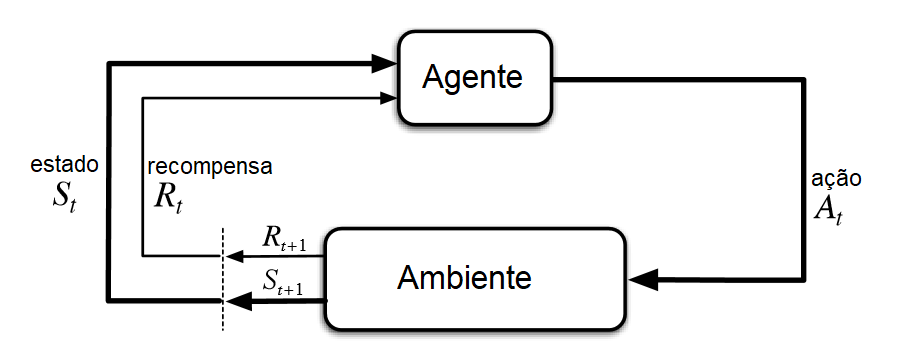
\includegraphics[width=0.60\textwidth]{fig/MDP.png}
 \caption{Exemplo de um Processo de Decisão de Markov (MDP).}
 \label{fig:mdp_ilustracao}
\end{figure}

Uma característica fundamental dos MDPs é a propriedade de Markov, que estabelece que a probabilidade de transição para um novo estado depende apenas do estado atual e da ação tomada, não dependendo de estados ou ações anteriores \cite{sutton}.

Os MDPs são amplamente utilizados em diversas áreas, incluindo:

\begin{itemize}
\item Robótica e controle automático
\item Planejamento de trajetórias
\item Gestão de recursos
\item Sistemas de recomendação
\item Jogos e simulações
\end{itemize}

Existem várias extensões dos MDPs para lidar com diferentes cenários:

\begin{itemize}
\item \textbf{POMDPs (Partially Observable MDPs)}: Lidam com situações onde o estado não é completamente observável.
\item \textbf{LLMDPs (Language-Limited MDPs)}: Incorporam restrições de linguagem nas ações e observações consideradas \cite{introducao_modelos_probabilisticos}.
\end{itemize}

Os MDPs fornecem uma base teórica sólida para o desenvolvimento de algoritmos de aprendizado por reforço, permitindo a modelagem e solução de problemas complexos de tomada de decisão sequencial sob incerteza.

\subsubsection{Funções de valor e política}
\label{subsubsec:valor_politica}

As funções de valor e política são conceitos fundamentais no aprendizado por reforço (RL), desempenhando papéis cruciais na tomada de decisões e na avaliação de estratégias. As funções de valor estimam o quão vantajoso é para um agente estar em um determinado estado ou executar uma ação específica em um estado. Existem dois tipos principais de funções de valor: a Função de Valor de Estado (V-function) e a Função de Valor de Ação (Q-function).

A Função de Valor de Estado, representada como \( V^\pi(s) \), indica o valor esperado de estar em um estado específico seguindo uma política \(\pi\). Matematicamente, é definida como \( V^\pi(s) = \mathbb{E}_\pi[G_t | S_t = s] \), onde \( G_t \) é o retorno acumulado a partir do tempo \( t \). Por outro lado, a Função de Valor de Ação, representada como \( Q^\pi(s,a) \), indica o valor esperado de tomar uma ação específica em um estado específico e depois seguir uma política \(\pi\). Sua definição matemática é \( Q^\pi(s,a) = \mathbb{E}_\pi[G_t | S_t = s, A_t = a] \).

Essas funções de valor são essenciais para métodos baseados em valor, como Q-learning e DQN (Deep Q-Network) \cite{0fe19b1631b60807bffb7757865b184d797c3016}. Elas permitem que o agente avalie a qualidade das ações em diferentes estados, facilitando a tomada de decisões ótimas.

As funções de política, por sua vez, definem o comportamento do agente, mapeando estados para ações. Existem dois tipos principais de políticas: a Política Determinística e a Política Estocástica. A Política Determinística mapeia cada estado para uma única ação, representada como \(\pi(s) = a\). Já a Política Estocástica mapeia cada estado para uma distribuição de probabilidade sobre as ações, representada como \(\pi(a|s) = P(A_t = a | S_t = s)\).

As funções de política são centrais para métodos baseados em política, como Policy Gradient e PPO (Proximal Policy Optimization) \cite{0fe19b1631b60807bffb7757865b184d797c3016}. Elas permitem que o agente aprenda diretamente qual ação tomar em cada estado, sem necessariamente estimar valores de estado ou ação.

A relação entre funções de valor e política é estreita. A função de valor avalia a qualidade de uma política, enquanto a política pode ser derivada da função de valor, por exemplo, escolhendo a ação com o maior valor \( Q \) em cada estado. Alguns métodos, como os algoritmos ator-crítico, combinam ambos os conceitos: o "ator" (política) decide quais ações tomar, e o "crítico" (função de valor) avalia essas ações e fornece feedback para melhorar a política \cite{0fe19b1631b60807bffb7757865b184d797c3016}.

O objetivo do RL é encontrar a política ótima \(\pi^*\) que maximize o retorno esperado. Isso pode ser alcançado de várias maneiras: métodos baseados em valor aprendem a função de valor ótima e derivam a política ótima a partir dela \cite{54807143779fa04466a0b0d01f4d1ecc94eb39ae}; métodos baseados em política otimizam diretamente a política, muitas vezes usando gradientes de política \cite{0fe19b1631b60807bffb7757865b184d797c3016}; e métodos híbridos combinam aprendizado de valor e otimização de política, como em algoritmos ator-crítico \cite{1911.04094}.

Recentes avanços incluem o uso de redes neurais profundas para aproximar funções de valor e política em ambientes complexos, como demonstrado no jogo de Hex \cite{54807143779fa04466a0b0d01f4d1ecc94eb39ae}, e o desenvolvimento de métodos robustos para lidar com incertezas e riscos em ambientes desafiadores \cite{2312.00342}.

As funções de valor e política são elementos cruciais no aprendizado por reforço (RL), especialmente em algoritmos avançados como o Proximal Policy Optimization (PPO). No PPO, as funções de valor são utilizadas para estimar a vantagem, que é essencial para o processo de otimização da política. A política, por sua vez, é ajustada para maximizar uma função objetivo surrogate, garantindo que as atualizações sejam estáveis e eficientes. Essa interação entre funções de valor e política permite que o PPO aprenda de forma eficaz em ambientes complexos, equilibrando desempenho e estabilidade. Vamos explorar esses conceitos e sua relação com o PPO.


\subsection{Aprendizado por Reforço Profundo}
\label{subsec:deep_rl}

O Aprendizado por Reforço Profundo (Deep Reinforcement Learning - DRL) é uma abordagem avançada de aprendizado de máquina que combina os princípios do aprendizado por reforço tradicional com as capacidades das redes neurais profundas. Esta técnica tem ganhado destaque significativo nos últimos anos devido à sua eficácia em resolver problemas complexos de tomada de decisão sequencial.

O Aprendizado por Reforço Profundo é um paradigma de aprendizado de máquina no qual um agente aprende a tomar decisões ótimas através da interação com um ambiente, utilizando redes neurais profundas para representar e processar informações complexas \cite{https://www.semanticscholar.org/paper/3879ab51e5eea7ce06dc31edbb169afb76e0bd71,https://www.semanticscholar.org/paper/45ae19e1e9037e10e90423b536eb183dcd99bd2e}. O objetivo principal é maximizar uma recompensa cumulativa ao longo do tempo, permitindo que o agente aprenda políticas de ação eficazes em ambientes dinâmicos e de alta dimensionalidade.

Uma característica fundamental do DRL é o aprendizado baseado em experiência. O agente aprende através da interação direta com o ambiente, acumulando experiência ao longo do tempo \cite{https://www.semanticscholar.org/paper/8efe27f4a31ebb72e9b3047107a4fe940259aad9}. As decisões são tomadas com base em um processo de tentativa e erro, onde o agente explora diferentes ações e aprende com os resultados obtidos.

Além disso, o DRL utiliza redes neurais profundas para processar e representar informações de alta dimensionalidade, como imagens ou dados sensoriais complexos \cite{https://www.semanticscholar.org/paper/8efe27f4a31ebb72e9b3047107a4fe940259aad9,https://www.semanticscholar.org/paper/3340124e85d6e5fbc08db49ad3e6a8d9ffa04222}. Isso permite a extração automática de características relevantes do ambiente, eliminando a necessidade de engenharia manual de recursos.

Outra característica importante é a adaptabilidade. O agente pode se adaptar a mudanças no ambiente e generalizar seu aprendizado para situações não vistas anteriormente \cite{https://www.semanticscholar.org/paper/27c834620d2c6adb51dffc4be9907e185907ce12}. O DRL é capaz de lidar com problemas parcialmente observáveis, onde nem toda a informação sobre o estado do ambiente está disponível.

O DRL também foca na otimização de longo prazo, buscando maximizar a recompensa cumulativa ao longo do tempo, em vez de apenas recompensas imediatas \cite{https://www.semanticscholar.org/paper/45ae19e1e9037e10e90423b536eb183dcd99bd2e}. Isso permite o aprendizado de estratégias complexas que envolvem planejamento e tomada de decisão em múltiplos passos.

Um dos desafios do DRL é balancear a necessidade de explorar novas ações para descobrir melhores estratégias com a exploração de ações conhecidas que já produzem bons resultados \cite{https://www.semanticscholar.org/paper/fef82649815694167ef56929648a51f2eb0849e9}. Técnicas como ε-greedy ou amostragem de Thompson são utilizadas para gerenciar este trade-off.

O Aprendizado por Reforço Profundo tem sido aplicado com sucesso em diversas áreas, incluindo navegação autônoma de robôs e veículos \cite{https://www.semanticscholar.org/paper/3340124e85d6e5fbc08db49ad3e6a8d9ffa04222,https://www.semanticscholar.org/paper/fef82649815694167ef56929648a51f2eb0849e9}, jogos eletrônicos e simulações complexas \cite{https://www.semanticscholar.org/paper/3879ab51e5eea7ce06dc31edbb169afb76e0bd71}, otimização de sistemas de controle industrial \cite{https://www.semanticscholar.org/paper/27c834620d2c6adb51dffc4be9907e185907ce12}, negociação automatizada em mercados financeiros \cite{https://www.semanticscholar.org/paper/45ae19e1e9037e10e90423b536eb183dcd99bd2e}, e gerenciamento de redes de comunicação e IoT \cite{https://www.semanticscholar.org/paper/3879ab51e5eea7ce06dc31edbb169afb76e0bd71,https://www.semanticscholar.org/paper/668a75bdb9c3f6d088f7da2b4b76ec1e66c484b8}.

Apesar de seu potencial, o DRL também enfrenta desafios significativos, como alta demanda computacional e longo tempo de treinamento \cite{https://www.semanticscholar.org/paper/8efe27f4a31ebb72e9b3047107a4fe940259aad9}, dificuldade em transferir o aprendizado de ambientes simulados para o mundo real \cite{https://www.semanticscholar.org/paper/fef82649815694167ef56929648a51f2eb0849e9}, sensibilidade a hiperparâmetros e configurações de treinamento \cite{https://www.semanticscholar.org/paper/3879ab51e5eea7ce06dc31edbb169afb76e0bd71}, e a necessidade de grandes quantidades de dados e interações para aprendizado efetivo.


\subsubsection{Redes neurais como aproximadores de função}
\label{subsubsec:redes_neurais}

As redes neurais como aproximadores de função desempenham um papel fundamental no contexto do Aprendizado por Reforço Profundo (DRL), representando uma das principais diferenças em relação ao aprendizado por reforço tradicional. Esta abordagem permite que os agentes de DRL lidem com espaços de estado e ação contínuos e de alta dimensionalidade, superando limitações significativas dos métodos tabulares convencionais.


No DRL, as redes neurais são utilizadas para aproximar funções complexas que mapeiam estados para valores (função de valor) ou ações (função de política). Essa capacidade de aproximação é crucial por várias razões:

1. \textbf{Generalização}: As redes neurais podem generalizar para estados não vistos anteriormente, interpolando ou extrapolando com base em padrões aprendidos.

2. \textbf{Compressão de Informação}: Permitem representar funções complexas de forma compacta, evitando a necessidade de armazenar valores para cada estado possível.

3. \textbf{Aprendizado de Características}: Extraem automaticamente características relevantes dos dados de entrada, eliminando a necessidade de engenharia manual de recursos.


\textbf{Aproximação da Função de Valor}: As redes neurais são utilizadas para estimar o valor esperado de estados ou pares estado-ação. Isso é particularmente útil em algoritmos como o Deep Q-Network (DQN), onde a rede neural aproxima a função Q, que representa o valor de longo prazo de tomar uma ação específica em um determinado estado.

\textbf{Aproximação da Função de Política}: Em métodos baseados em política, como o PPO (Proximal Policy Optimization), as redes neurais são usadas para representar diretamente a política do agente. Elas mapeiam estados para distribuições de probabilidade sobre ações, permitindo que o agente tome decisões em ambientes contínuos ou de alta dimensionalidade.

\textbf{Modelos de Ambiente}: Em algumas abordagens de DRL baseadas em modelo, as redes neurais são usadas para aproximar a dinâmica do ambiente, prevendo estados futuros e recompensas com base em estados e ações atuais.


As vantagens incluem a capacidade de lidar com espaços de estado e ação contínuos, a habilidade de processar entradas de alta dimensionalidade, como imagens ou dados sensoriais complexos, e o potencial para transferência de aprendizado entre tarefas similares. 

Os desafios envolvem a instabilidade de treinamento devido à não-estacionariedade do processo de aprendizagem, o overfitting em conjuntos de dados limitados, e a dificuldade em interpretar as decisões do modelo devido à natureza de "caixa preta" das redes neurais profundas.


No contexto do PPO, as redes neurais são utilizadas tanto para aproximar a função de política quanto para estimar a função de valor. A política é representada por uma rede neural que mapeia estados para distribuições de probabilidade sobre ações, enquanto uma segunda rede (ou uma rede compartilhada com saídas separadas) estima o valor de cada estado.

O uso de redes neurais como aproximadores de função no PPO permite que o algoritmo lide eficientemente com ambientes complexos e contínuos. A técnica de clipping do PPO, que limita as mudanças na política, ajuda a estabilizar o treinamento dessas redes neurais, mitigando alguns dos desafios associados à aproximação de função em DRL.


\subsection{Proximal Policy Optimization (PPO)}
\label{subsec:ppo}

\subsubsection{Motivação e princípios do PPO}
\label{subsubsec:ppo_principios}

O Proximal Policy Optimization (PPO) surgiu como uma resposta às limitações dos algoritmos de aprendizado por reforço anteriores, visando melhorar a estabilidade e eficiência do treinamento em ambientes complexos. O PPO foi desenvolvido para abordar os desafios de otimização de políticas em espaços de ação contínuos e de alta dimensionalidade, comuns em problemas do mundo real\cite{https://arxiv.org/abs/2404.02577}.

Os princípios fundamentais do PPO incluem:

1. Atualização conservadora de política: O PPO busca realizar atualizações de política que sejam significativas, mas não excessivamente grandes, para evitar colapsos de desempenho.

2. Equilíbrio entre exploração e aproveitamento: O algoritmo mantém um equilíbrio entre explorar novas ações e aproveitar as ações conhecidas que produzem bons resultados.

3. Eficiência amostral: O PPO é projetado para aprender de forma eficiente a partir de experiências limitadas, reduzindo a quantidade de dados necessários para o treinamento.

\subsubsection{Função objetivo e mecanismo de clipping}
\label{subsubsec:ppo_objetivo}

A função objetivo do PPO é projetada para incentivar melhorias na política enquanto evita mudanças drásticas. O componente central desta função é o mecanismo de clipping, que limita a magnitude das atualizações de política\cite{https://pubmed.ncbi.nlm.nih.gov/33705327}.

A função objetivo do PPO pode ser expressa como:

$$
L^{CLIP}(\theta) = \mathbb{E}_t[\min(r_t(\theta)\hat{A}_t, \text{clip}(r_t(\theta), 1-\epsilon, 1+\epsilon)\hat{A}_t)]
$$

Onde:
- \(r_t(\textbf{\theta})\) é a razão entre a nova e a antiga probabilidade de ação

- \(\hat{A}_t\) é a estimativa de vantagem

- \(\epsilon\) é o parâmetro de clipping

O mecanismo de clipping garante que a razão de probabilidade $$r_t(\theta)$$ permaneça dentro de um intervalo $$[1-\epsilon, 1+\epsilon]$$, impedindo atualizações excessivamente grandes na política. Isso promove uma aprendizagem mais estável e reduz o risco de colapso de desempenho durante o treinamento\cite{https://www.semanticscholar.org/paper/df03d874a7bfff4fb3a769c2c3615c034cc268f1}.

\subsubsection{Vantagens do PPO em ambientes contínuos e multiagentes}
\label{subsubsec:ppo_vantagens}

O PPO demonstra várias vantagens em ambientes contínuos e multiagentes:

1. Estabilidade em espaços de ação contínuos: O PPO é particularmente eficaz em problemas com espaços de ação contínuos, como controle robótico e navegação autônoma\cite{https://arxiv.org/abs/2404.02577,https://arxiv.org/abs/1710.04423}.

2. Escalabilidade para sistemas multiagentes: O algoritmo se adapta bem a cenários com múltiplos agentes, permitindo a coordenação eficiente em ambientes complexos\cite{https://www.semanticscholar.org/paper/bb51dbfb79919e392709be5c7b8f8119fe3f9420}.

3. Eficiência computacional: Comparado a métodos centralizados, o PPO oferece vantagens em termos de complexidade computacional, garantindo tempos de planejamento curtos em ambientes de larga escala\cite{https://www.semanticscholar.org/paper/133b58d42562ce16d99fad0e59d3edeff515821c}.

4. Adaptabilidade a diferentes números de agentes: Políticas aprendidas com PPO demonstram boa escalabilidade, podendo ser aplicadas a diferentes números de agentes sem perda significativa de desempenho\cite{https://www.semanticscholar.org/paper/bb51dbfb79919e392709be5c7b8f8119fe3f9420}.

5. Robustez em tarefas de longo prazo: O PPO é capaz de lidar com recompensas extremamente atrasadas e horizontes de tempo longos, tornando-o adequado para tarefas complexas do mundo real\cite{https://arxiv.org/abs/2404.02577}.

6. Flexibilidade na engenharia de recompensas: O PPO permite a incorporação de mecanismos sofisticados de recompensa, como recompensas de densidade e penalidades de etapas, para melhorar a eficiência da tarefa e reduzir comportamentos indesejados\cite{https://www.semanticscholar.org/paper/133b58d42562ce16d99fad0e59d3edeff515821c}.

Essas vantagens tornam o PPO uma escolha popular para uma ampla gama de aplicações, desde jogos e robótica até sistemas de transporte e otimização de processos industriais\cite{https://arxiv.org/abs/2404.02577,https://www.semanticscholar.org/paper/c70691776f1c755a5f7c00dbf8929e2b61a0a240,https://www.semanticscholar.org/paper/bb51dbfb79919e392709be5c7b8f8119fe3f9420}.

%% - - - - - - - - - - - - - - - - - - - - - - - - - - - - - - - - - - -
\section{Aprendizado por Reforço Multiagente}
\label{sec:marl}

No contexto de aprendizado por reforço (reinforcement learning) e aprendizado por reforço profundo (deep reinforcement learning), vamos detalhar os conceitos solicitados:

O Aprendizado por Reforço Multiagente (Multi-Agent Reinforcement Learning - MARL) é uma extensão do aprendizado por reforço tradicional que lida com ambientes onde múltiplos agentes interagem simultaneamente\cite{https://arxiv.org/abs/2412.21088,https://arxiv.org/abs/2401.10949}. Nesse cenário, os agentes devem aprender a tomar decisões ótimas considerando não apenas o ambiente, mas também as ações e estratégias dos outros agentes.

No MARL, cada agente busca maximizar sua própria recompensa, mas suas ações afetam o ambiente compartilhado e, consequentemente, as recompensas dos outros agentes\cite{https://www.semanticscholar.org/paper/c6c4198ac541ce339e76feb8ca2de813acb87fc2}. Isso cria um cenário complexo onde a cooperação e a competição entre agentes desempenham papéis cruciais.

\subsection{Desafios em Ambientes Multiagente}
\label{subsec:desafios_multi}

\subsubsection{Coordenação e competição entre agentes}
\label{subsubsec:coordenacao}

A coordenação e competição entre agentes são aspectos fundamentais do MARL que apresentam desafios significativos:

1. Coordenação: Em cenários cooperativos, os agentes precisam aprender a trabalhar juntos para atingir objetivos comuns\cite{https://arxiv.org/abs/2410.21290}. Isso envolve:
   - Desenvolvimento de estratégias conjuntas
   - Compartilhamento de informações relevantes
   - Sincronização de ações para maximizar a eficiência coletiva

2. Competição: Em ambientes competitivos ou mistos, os agentes podem ter objetivos conflitantes\cite{https://www.semanticscholar.org/paper/c6c4198ac541ce339e76feb8ca2de813acb87fc2}. Isso leva a:
   - Necessidade de prever e reagir às ações dos oponentes
   - Desenvolvimento de estratégias robustas contra adversários adaptativos
   - Equilíbrio entre cooperação e competição em cenários mistos

Para lidar com esses desafios, técnicas como o uso de métricas de alinhamento de políticas baseadas na distância de Wasserstein têm sido propostas para melhorar a coordenação entre agentes\cite{https://arxiv.org/abs/2401.10949}.

\subsubsection{Não-estacionariedade do ambiente}
\label{subsubsec:nao_estacionariedade}

A não-estacionariedade é um dos principais desafios em MARL e refere-se à mudança constante do ambiente do ponto de vista de cada agente individual\cite{https://arxiv.org/abs/2412.21088,https://www.semanticscholar.org/paper/96c58672ee781bf75246a039d781e2dc8af5f43e}. Isso ocorre porque:

1. Agentes em evolução: Cada agente está continuamente aprendendo e adaptando suas políticas, o que altera o ambiente para os outros agentes\cite{https://arxiv.org/abs/2412.20523}.

2. Dinâmica complexa: As interações entre múltiplos agentes criam uma dinâmica que é difícil de prever e modelar\cite{https://arxiv.org/abs/2410.21290}.

3. Observações parciais: Muitas vezes, os agentes têm acesso apenas a informações locais, o que dificulta a compreensão completa do estado do ambiente\cite{https://arxiv.org/abs/2410.21290}.

A não-estacionariedade apresenta vários desafios:

- Instabilidade na aprendizagem: As políticas que eram ótimas em um momento podem se tornar subótimas rapidamente.
- Exploração ineficiente: Estratégias de exploração eficazes em ambientes estacionários podem falhar em ambientes não-estacionários.
- Convergência difícil: A constante mudança no ambiente pode impedir que os agentes convirjam para políticas estáveis.

Para abordar a não-estacionariedade, pesquisadores têm proposto várias soluções:

- Uso de modelos do ambiente para prever mudanças e adaptar as políticas dos agentes\cite{https://www.semanticscholar.org/paper/96c58672ee781bf75246a039d781e2dc8af5f43e}.
- Desenvolvimento de algoritmos que consideram explicitamente a natureza não-estacionária do ambiente, como variantes do algoritmo MADDPG (Multi-Agent Deep Deterministic Policy Gradient)\cite{https://arxiv.org/abs/2410.21290}.
- Implementação de técnicas de comunicação entre agentes para melhorar a coordenação e adaptação às mudanças do ambiente\cite{https://arxiv.org/abs/2410.21290}.

Essas abordagens visam melhorar a robustez e a eficácia dos sistemas de MARL em ambientes complexos e dinâmicos, permitindo que os agentes aprendam e se adaptem de forma mais eficiente em cenários multiagente desafiadores.

% \subsection{Aplicações em Futebol de Robôs}
% \label{subsec:futebol_robos}

% \subsubsection{Visão geral da categoria SSL-EL}
% \label{subsubsec:ssl_el}

% \subsubsection{Desafios específicos do domínio}
% \label{subsubsec:desafios_dominio}

%% - - - - - - - - - - - - - - - - - - - - - - - - - - - - - - - - - - -
\section{Técnicas de Aprendizado Progressivo}
\label{sec:aprendizado_prog}

No contexto de aprendizado por reforço (reinforcement learning) e aprendizado por reforço profundo (deep reinforcement learning), as técnicas de aprendizado progressivo são abordagens que visam melhorar a eficiência e eficácia do processo de aprendizagem dos agentes. O aprendizado progressivo, também conhecido como aprendizado incremental ou currículo de aprendizagem, é uma estratégia que facilita o aprendizado de tarefas complexas dividindo-as em subtarefas mais simples e gradualmente aumentando a dificuldade. Os princípios fundamentais dessa técnica incluem a decomposição de tarefas, onde o problema principal é dividido em subtarefas mais gerenciáveis, o sequenciamento, que organiza as subtarefas em uma ordem crescente de complexidade, e a transferência de conhecimento, onde o aprendizado adquirido em tarefas mais simples é utilizado como base para tarefas mais complexas. 

Implementações em RL e Deep RL incluem o currículo de aprendizagem, que inicia o treinamento com versões simplificadas do ambiente e gradualmente aumenta a complexidade à medida que o agente melhora seu desempenho, o aprendizado hierárquico, que utiliza uma estrutura hierárquica de políticas onde políticas de alto nível selecionam subtarefas e políticas de baixo nível executam ações específicas, a transferência de aprendizado, onde o conhecimento adquirido em tarefas similares é transferido para acelerar o aprendizado em novas tarefas, e o meta-aprendizado, onde o agente aprende a aprender, desenvolvendo estratégias gerais que podem ser rapidamente adaptadas a novas situações. Os benefícios dessas técnicas incluem um aprendizado mais rápido, melhor generalização, superação de mínimos locais e escalabilidade, permitindo abordar problemas mais complexos que seriam intratáveis com abordagens diretas. No entanto, desafios como o design do currículo, o equilíbrio entre exploração e aproveitamento, e a necessidade de evitar overfitting são aspectos críticos a serem considerados. As técnicas de aprendizado progressivo representam uma área promissora na pesquisa de RL e Deep RL, oferecendo caminhos para superar limitações tradicionais e abordar problemas cada vez mais complexos do mundo real\cite{https://www.semanticscholar.org/paper/3004b3eba73f4def2d36d2064eadc76c5244547d,https://www.semanticscholar.org/paper/f11594e47ce3f5872bd4d4868f23655025bb6511,https://www.semanticscholar.org/paper/b30e72c8f236951fe26024bfe49bda84e8bf133b,https://www.semanticscholar.org/paper/c984fdd5f847e46a9335c5aba982d31ceafbcb27,https://www.semanticscholar.org/paper/ece55442b2aee7f9db67c7fc58a6a857ed915fcd,https://www.semanticscholar.org/paper/801d0ef8c81c13a64228720b7d43660dcf664705,https://www.semanticscholar.org/paper/68fb81aa0a7d17ff07cb4c8d74cb78f0e67bbcca,https://www.semanticscholar.org/paper/1a4a43a3997e2694b6ce91ba33ebade1269a6256,https://www.semanticscholar.org/paper/67dd6e219a02aeb8f151eec2d8254e30cf7599dd}.

\subsection{Curriculum Learning}
\label{subsec:curriculum}

Curriculum Learning é uma abordagem de aprendizado progressivo inspirada na forma como os seres humanos aprendem, começando com conceitos simples e gradualmente progredindo para tarefas mais complexas. A motivação por trás dessa técnica é melhorar a eficiência e eficácia do processo de aprendizagem em ambientes de Reinforcement Learning (RL) e Deep Reinforcement Learning (Deep RL). Os princípios fundamentais do Curriculum Learning incluem a ordenação de tarefas do mais fácil ao mais difícil, o aprendizado gradual expondo o agente a desafios progressivamente mais complexos e a transferência de conhecimento de tarefas simples para problemas mais elaborados.

\subsubsection{Conceito e motivação}
\label{subsubsec:curriculum_conceito}

O conceito de Curriculum Learning baseia-se na ideia de que a aprendizagem pode ser facilitada ao estruturar o processo de ensino de maneira incremental. Isso significa que, ao invés de expor o agente a tarefas complexas desde o início, ele é inicialmente treinado em tarefas mais simples, que são gradualmente substituídas por tarefas mais difíceis à medida que o agente adquire habilidades e conhecimento. A motivação para essa abordagem é que ela pode levar a um aprendizado mais eficiente e eficaz, permitindo que o agente desenvolva uma base sólida de conhecimento antes de enfrentar desafios mais complexos. Essa técnica é particularmente útil em ambientes de RL e Deep RL, onde a complexidade das tarefas pode variar significativamente e a capacidade de transferir conhecimento de tarefas simples para problemas mais elaborados pode ser crucial para o sucesso do agente.

\subsubsection{Desenho de currículos para RL}
\label{subsubsec:curriculum_desenho}

O desenho de currículos eficazes para RL é um aspecto crucial do Curriculum Learning. Algumas estratégias incluem a modificação do ambiente, onde inicialmente o agente interage com versões simplificadas do ambiente, com a complexidade aumentando gradualmente. Outra estratégia é a seleção de tarefas, onde um algoritmo seleciona tarefas apropriadas baseadas no nível atual de habilidade do agente. Além disso, a estrutura de recompensas pode ser ajustada ao longo do tempo, começando com recompensas mais frequentes para comportamentos básicos e progredindo para recompensas mais esparsas focadas em comportamentos complexos. O design eficaz de um currículo frequentemente requer conhecimento especializado do domínio, e a automatização desse processo é uma área ativa de pesquisa\cite{https://www.semanticscholar.org/paper/79d92c9a3e0de40d863e43232e2c00370412a841}.

\subsubsection{Aplicações em robótica e jogos}
\label{subsubsec:curriculum_aplicacoes}

Curriculum Learning tem demonstrado resultados promissores em diversas aplicações, incluindo robótica e jogos. Em manipuladores robóticos, o Curriculum Learning tem sido aplicado para melhorar o aprendizado de tarefas complexas. Técnicas como Q-Learning, Deep Reinforcement Learning, Actor-Critic e Policy Gradient são frequentemente utilizadas nesse contexto\cite{https://www.semanticscholar.org/paper/f11594e47ce3f5872bd4d4868f23655025bb6511}. No campo dos jogos digitais educacionais, abordagens de aprendizado progressivo, como o Curriculum Learning, podem ser integradas com Game Learning Analytics para melhorar a experiência de aprendizado e o engajamento dos jogadores\cite{https://www.semanticscholar.org/paper/704147ceaed752c17e5f24f9a3521c41cbfc9ff7}. Além disso, estudos têm aplicado Curriculum Learning em experimentos de navegação autônoma, demonstrando como variações nos parâmetros de aprendizado, como taxa de aprendizado e fator de desconto, podem afetar significativamente o desempenho do agente\cite{https://www.semanticscholar.org/paper/79d92c9a3e0de40d863e43232e2c00370412a841}. O Curriculum Learning oferece benefícios significativos, incluindo aprendizado mais rápido, melhor generalização e superação de mínimos locais. No entanto, desafios como o design adequado do currículo e o balanceamento entre tarefas fáceis e difíceis permanecem áreas de pesquisa ativa no campo de RL e Deep RL.

\subsection{Self-Play}
\label{subsec:self_play}

\subsubsection{Princípios do self-play em RL}
\label{subsubsec:self_play_principios}

%\subsubsection{Geração automática de currículos via self-play}
%\label{subsubsec:self_play_curriculos}

\subsubsection{Exemplos de sucesso em jogos complexos}
\label{subsubsec:self_play_exemplos}

%% - - - - - - - - - - - - - - - - - - - - - - - - - - - - - - - - - - -
% \section{Integração de Técnicas para Aquisição Progressiva de Habilidades}
% \label{sec:integracao}

% \subsection{Combinando Curriculum Learning e Self-Play}
% \label{subsec:combinacao}

% \subsubsection{Sinergias entre as abordagens}
% \label{subsubsec:sinergias}

% \subsubsection{Desafios na integração}
% \label{subsubsec:desafios_integracao}

% \subsection{Aplicação ao Futebol de Robôs Multiagente}
% \label{subsec:aplicacao_futebol}

% \subsubsection{Desenho de currículos para habilidades de futebol}
% \label{subsubsec:curriculos_futebol}

% \subsubsection{Transição do curriculum para self-play competitivo}
% \label{subsubsec:transicao_self_play}

% \subsubsection{Potenciais benefícios na aquisição de habilidades complexas}
% \label{subsubsec:beneficios_aquisicao}
\chapter{Metodologia}
\label{cap:metodologia}

\section{Ambiente de Simulação}
\label{sec:ambiente_simulacao}

O ambiente de simulação utilizado neste trabalho é o \textit{RL-SSL-EL}\footnote{\url{https://github.com/Werikcyano/RL-SSL-EL}} na versão de implementação da equipe de robótica Pequi Mecânico, conforme ilustrado na Figura \ref{fig:campo_simulacao}. \textit{RL-SSL-EL} é uma plataforma de simulação específica para o futebol de robôs na categoria \textit{Small Size League - Entry League (SSL-EL)}. Esta plataforma foi projetada para simplificar o processo de aprendizado por reforço aplicado ao futebol de robôs, oferecendo uma abstração adequada dos desafios físicos e técnicos básicos que são inerentes a este domínio.

\begin{figure}[h]
    \centering
    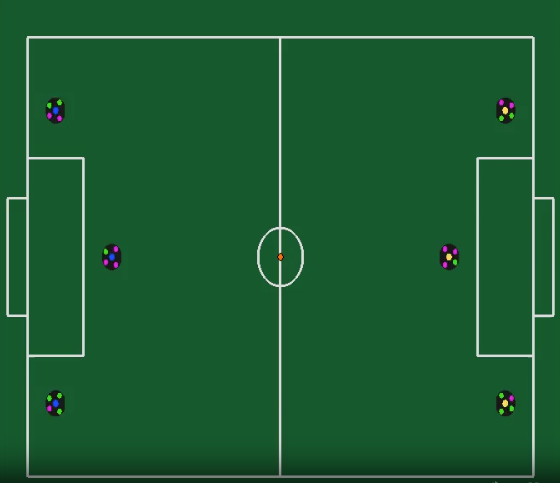
\includegraphics[width=0.8\textwidth]{fig/campo}
    \caption{Visualização do ambiente de simulação \textit{RL-SSL-EL} mostrando o campo de jogo com os robôs e a bola}
    \label{fig:campo_simulacao}
\end{figure}

\subsection{Características e Limitações}

O ambiente \textit{RL-SSL-EL} utiliza a biblioteca \textit{RLlib} para implementação dos algoritmos de aprendizado por reforço, o que permite a aplicação de técnicas como \textit{Proximal Policy Optimization (PPO)} de forma distribuída e eficiente. A simulação opera com base no modelo físico do futebol de robôs, incluindo movimentação dos robôs, dinâmica da bola, e interações entre os agentes no campo.

Entre as principais características do ambiente, destacam-se:

\begin{itemize}
    \item Compatibilidade com o \textit{framework RLlib} para treinamento distribuído;
    \item Suporte a múltiplos agentes na arquitetura multiagente;
    \item Sistema de recompensas configurável;
    \item Métricas de avaliação em tempo real;
    \item Capacidade de visualização do ambiente durante o treinamento.
\end{itemize}

As limitações mais relevantes incluem a simplificação dos aspectos físicos da simulação em comparação com ambientes mais complexos, e restrições nas estratégias de posicionamento dos robôs. Estas limitações, embora relevantes, não comprometem significativamente os objetivos deste trabalho, que foca principalmente na avaliação da eficácia do \textit{curriculum learning} em comparação com a abordagem \textit{self-play} convencional.

\subsection{Configurações Utilizadas}

O ambiente foi configurado para reproduzir um cenário de jogo simplificado, com parâmetros adequados para o treinamento efetivo dos agentes. As principais configurações incluem:

\begin{itemize}
    \item Frequência de atualização: 30 \textit{FPS} (\textit{frames} por segundo);
    \item Duração dos episódios: 40 segundos de jogo simulado;
    \item Número de agentes por equipe: 3 robôs (configurável conforme o estágio do \textit{curriculum});
    \item Posicionamento inicial: configurável para cada agente e para a bola;
    \item Limite de passos por episódio: variável conforme o estágio do \textit{curriculum} (300 a 500 passos).
\end{itemize}

Estas configurações foram ajustadas para oferecer um equilíbrio entre complexidade suficiente para o aprendizado significativo e simplicidade necessária para viabilizar o treinamento eficiente.

\section{Arquitetura do Sistema}
\label{sec:arquitetura_sistema}

\subsection{Modelo Base (\textit{Self-play Default})}

O sistema base utiliza a abordagem \textit{self-play} para treinamento dos agentes de futebol de robôs. Nesta abordagem, uma única política é treinada e utilizada tanto para os robôs da equipe azul (agentes em treinamento) quanto para a equipe amarela (oponentes). Esta configuração permite que os agentes evoluam continuamente, enfrentando versões cada vez mais competentes de si mesmos.

A arquitetura do sistema \textit{self-play} é implementada na classe \texttt{SelfPlayUpdateCallback}, responsável por gerenciar a atualização dos pesos da política dos oponentes. O funcionamento básico deste sistema segue os seguintes princípios:

\begin{enumerate}
    \item Uma política neural é treinada para os agentes da equipe azul;
    \item Uma cópia desta política é periodicamente transferida para os agentes da equipe amarela;
    \item A atualização ocorre quando a política azul atinge um nível de desempenho superior predefinido;
    \item A métrica utilizada para decidir sobre a atualização é baseada na diferença de pontuação entre as equipes.
\end{enumerate}

Este processo cria um ciclo virtuoso de melhoria contínua, onde os agentes constantemente enfrentam oponentes que representam desafios adequados ao seu nível de habilidade atual.

\subsection{Adaptações Propostas por Este Trabalho}

Este trabalho propõe uma adaptação significativa ao sistema base, com a introdução do \textit{curriculum learning} como uma fase preparatória para o \textit{self-play}. Esta modificação visa estabelecer uma progressão mais estruturada no aprendizado dos agentes, permitindo que eles desenvolvam habilidades fundamentais antes de serem expostos aos desafios completos do futebol de robôs competitivo.

As principais adaptações incluem:

\begin{enumerate}
    \item Implementação da classe \texttt{SSLCurriculumEnv}, que estende a classe base \texttt{SSLMultiAgentEnv} para suportar diferentes níveis de complexidade no treinamento;
    
    \item Desenvolvimento do \texttt{CurriculumCallback}, responsável por monitorar o desempenho dos agentes e controlar a progressão entre os níveis do \textit{curriculum};
    
    \item Criação de um sistema de configuração modular para os diferentes estágios do \textit{curriculum}, permitindo ajustes precisos nos parâmetros de cada nível;
    
    \item Implementação de métricas específicas para avaliar o desempenho dos agentes em cada estágio do \textit{curriculum}.
\end{enumerate}

Estas adaptações permitem uma transição suave do treinamento estruturado para o ambiente competitivo, potencialmente melhorando a eficiência do aprendizado e a qualidade das políticas resultantes.

\subsection{Pipeline de Treinamento}

O \textit{pipeline} de treinamento implementado neste trabalho integra o \textit{curriculum learning} e o \textit{self-play} em uma sequência coerente, permitindo que os agentes progridam de forma gradual de tarefas simples até o jogo completo. A Figura \ref{fig:fluxograma_treino} apresenta uma visão geral deste processo, ilustrando a estrutura do \textit{pipeline} e a interação entre seus componentes.

\begin{figure}[H]
    \centering
    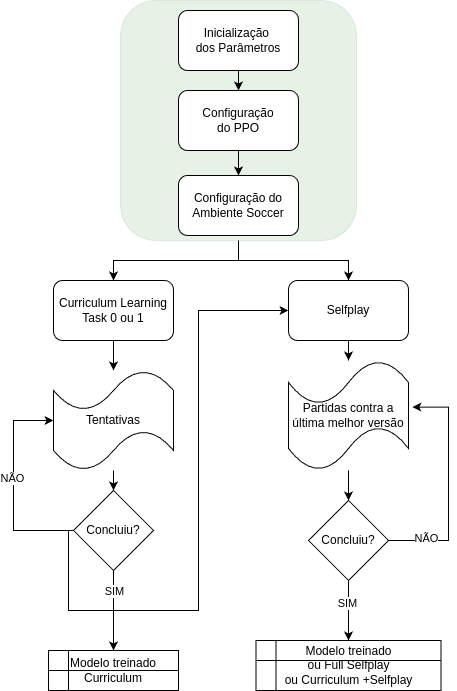
\includegraphics[width=0.85\textwidth]{fig/fluxograma_treino_mestrado.png}
    \caption{Fluxograma do \textit{pipeline} de treinamento, destacando a integração entre \textit{Curriculum Learning} e \textit{Self-play}. O processo inicia com a inicialização e configuração dos componentes, seguido pela divisão entre as abordagens de \textit{Curriculum Learning} e \textit{Self-play} direto. A fase de \textit{Curriculum Learning} inclui tarefas progressivas (\textit{Task} 0 ou 1) seguidas por ciclos de tentativas até conclusão do critério de promoção, resultando em um modelo treinado que serve como base para o \textit{Self-play} subsequente. Fonte: Elaborado pelo autor.}
    \label{fig:fluxograma_treino}
\end{figure}

Como ilustrado no fluxograma, este \textit{pipeline} é composto por três estágios principais:

\begin{enumerate}
    \item \textbf{Treinamento com \textit{Curriculum Learning}}: Os agentes iniciam o treinamento em um ambiente simplificado, com tarefas específicas de complexidade progressiva (\textit{Task} 0 ou 1). Este estágio utiliza o \texttt{CurriculumCallback} para monitorar o desempenho e controlar a progressão através de ciclos de tentativas até que os critérios de conclusão sejam atingidos.
    
    \item \textbf{Transição para \textit{Self-play}}: Após completar os estágios do \textit{curriculum}, os agentes são transferidos para o ambiente de \textit{self-play}, onde enfrentam versões anteriores de si mesmos como oponentes.
    
    \item \textbf{Refinamento com \textit{Self-play}}: Os agentes continuam o treinamento no ambiente competitivo, com atualizações periódicas da política dos oponentes quando alcançam níveis de desempenho predefinidos, através de partidas contra a última melhor versão.
\end{enumerate}

A implementação deste processo de treinamento é feita através de um arquivo central que organiza e coordena todas as etapas necessárias. Este arquivo é responsável por configurar o ambiente de treinamento e definir como os robôs devem se comportar em cada fase. A mudança entre as diferentes fases do treinamento pode ser facilmente ajustada através de configurações específicas, permitindo maior flexibilidade durante todo o processo.

\section{Implementação do \textit{Curriculum Learning}}
\label{sec:implementacao_cl}

\subsection{Visão Geral da Arquitetura do \textit{Curriculum}}

A arquitetura do \textit{curriculum learning} implementada neste trabalho segue uma estrutura de estágios progressivos, onde cada estágio representa um nível de complexidade específico no aprendizado do futebol de robôs. A progressão entre estes estágios é controlada por critérios de desempenho predefinidos, garantindo que os agentes desenvolvam as habilidades necessárias antes de avançar para desafios mais complexos.

A transição do cenário curricular é projetada para preservar a continuidade do aprendizado, evitando mudanças abruptas que poderiam prejudicar o desenvolvimento dos agentes. Esta arquitetura foi inspirada em sistemas de treinamento progressivo observados em jogos eletrônicos populares, como FIFA e \textit{Rocket League}, onde os jogadores são introduzidos gradualmente a conceitos mais complexos.

\begin{figure}[H]
    \centering
    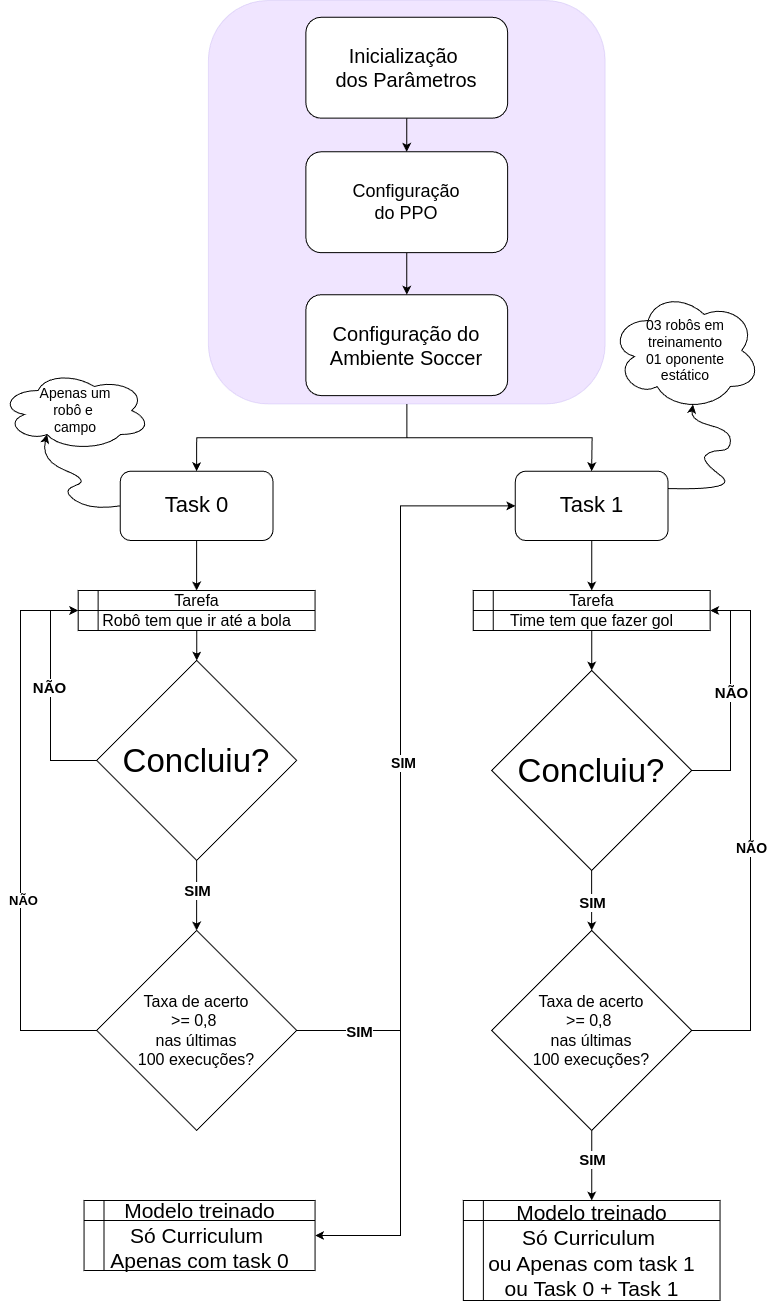
\includegraphics[width=0.85\textwidth]{fig/fluxograma_treino_curriculum.png}
    \caption{Diagrama de fluxo do processo de treinamento com \textit{curriculum learning}. Fonte: Elaborado pelo autor.}
    \label{fig:diagrama_curriculum}
\end{figure}

O fluxo do processo inicia com a definição dos estágios e seus respectivos parâmetros no arquivo de configuração \texttt{config.yaml}. Estes parâmetros incluem critérios de sucesso, sistemas de recompensa específicos, e configurações do ambiente para cada estágio. Durante o treinamento, o \texttt{CurriculumCallback} monitora continuamente o desempenho dos agentes, calculando a taxa de sucesso com base em uma janela deslizante de episódios recentes. Quando esta taxa atinge o limiar de promoção predefinido, o sistema avança automaticamente para o próximo estágio do \textit{curriculum}.

\subsection{Estrutura dos Estágios}

O \textit{curriculum} implementado neste trabalho é estruturado em três estágios principais, cada um representando um nível distinto de complexidade no aprendizado do futebol de robôs. Estes estágios são designados como tarefas (\textit{tasks}) e numerados de 0 a 1, com cada tarefa apresentando configurações e objetivos específicos.

\subsubsection{Estágio 1 (\textit{Task} 0): Fundamentos Básicos}
\label{subsubsec:estagio1}

O Estágio 1 representa o nível mais básico do \textit{curriculum}, focado no desenvolvimento de habilidades fundamentais sem a presença de oponentes. Neste estágio, os agentes aprendem a se aproximar e interagir com a bola em um ambiente controlado.

\paragraph{Configuração do Ambiente}

No Estágio 1, o ambiente é configurado com as seguintes características:
\begin{itemize}
    \item Um robô da equipe azul, posicionado em local predefinido;
    \item Ausência de robôs oponentes (equipe amarela);
    \item Bola posicionada no centro do campo;
    \item Limite de 300 passos por episódio.
\end{itemize}

\paragraph{Sistema de Recompensas}

O sistema de recompensas para este estágio é simplificado, focando primariamente no contato com a bola. A estrutura de recompensas inclui:
\begin{itemize}
    \item Recompensa principal (10 pontos) concedida quando um agente toca na bola;
    \item Recompensas incrementais relacionadas à aproximação da bola;
    \item Penalidades por tempo excessivo sem interação com a bola.
\end{itemize}

\paragraph{Critérios de Progressão}

Para avançar deste estágio para o próximo, os agentes devem demonstrar consistência em sua capacidade de interagir com a bola. Especificamente:
\begin{itemize}
    \item Taxa de sucesso de pelo menos 80\% em uma janela de 100 episódios;
    \item O sucesso é definido como tocar na bola pelo menos uma vez durante o episódio.
\end{itemize}

\subsubsection{Estágio 2 (\textit{Task} 1): Interação com Oponentes Estáticos}
\label{subsubsec:estagio2}

O Estágio 2 introduz um nível intermediário de complexidade, apresentando oponentes estáticos e objetivos táticos mais elaborados. Neste estágio, os agentes precisam aprender a navegar em um ambiente com obstáculos e realizar ações mais coordenadas.

\paragraph{Configuração do Ambiente}

O ambiente neste estágio apresenta as seguintes características:
\begin{itemize}
    \item Três robôs da equipe azul, mantendo a formação básica com pequena variação nas posições;
    \item Um robô oponente (equipe amarela), posicionado estrategicamente próximo à bola;
    \item Bola posicionada no centro, com variações aleatórias limitadas;
    \item Limite de 400 passos por episódio.
\end{itemize}

\paragraph{Sistema de Recompensas}

O sistema de recompensas é expandido para incluir objetivos táticos mais avançados:
\begin{itemize}
    \item Recompensa por proximidade à bola (10\% do peso total);
    \item Recompensa por conduzir a bola em direção ao gol adversário (30\% do peso);
    \item Recompensa substancial por marcar gols (10 pontos);
    \item Recompensa menor por manter posse de bola (5\% do peso).
\end{itemize}

\paragraph{Critérios de Progressão}

A progressão para o próximo estágio requer habilidades táticas mais avançadas:
\begin{itemize}
    \item Taxa de sucesso de pelo menos 80\% em uma janela de 100 episódios;
    \item O sucesso neste estágio é definido como marcar pelo menos um gol durante o episódio.
\end{itemize}

%\subsubsection{Estágio 3 (\textit{Task} 2): Jogo Completo com Oponentes Ativos}
%\label{subsubsec:estagio3}

%O Estágio 3 representa o nível mais avançado do \textit{curriculum}, introduzindo múltiplos oponentes ativos e aproximando-se das condições reais de jogo. Neste estágio, os agentes precisam demonstrar capacidades táticas complexas e coordenação de equipe.

%\paragraph{Configuração do Ambiente}

%O ambiente neste estágio apresenta complexidade máxima:
%\begin{itemize}
%    \item Três robôs da equipe azul, com posicionamento tático
%    \item Três robôs oponentes (equipe amarela), distribuídos estrategicamente pelo campo
%    \item Posições iniciais configuradas para simular situações táticas realistas
%    \item Limite de 500 passos por episódio
%\end{itemize}

%\paragraph{Sistema de Recompensas}

%O sistema de recompensas é refinado para valorizar aspectos estratégicos do jogo:
%\begin{itemize}
%    \item Manutenção das recompensas por proximidade à bola e ao gol
%    \item Valorização adicional de comportamentos defensivos quando necessário
%    \item Penalizações por violações das regras (saída da bola, faltas)
%    \item Recompensas por posicionamento tático eficiente
%\end{itemize}

\paragraph{Transição para \textit{Self-play}}

Após completar este estágio, os agentes são considerados preparados para o treinamento \textit{self-play}, onde enfrentarão versões cada vez mais competentes de si mesmos. Esta transição marca a conclusão do \textit{curriculum} estruturado e o início da fase competitiva do treinamento.

\subsection{Mecanismo de Transição entre Estágios}
\label{subsec:mecanismo_transicao}

O mecanismo de transição entre os estágios do \textit{curriculum} é implementado na classe \texttt{CurriculumCallback}, responsável por monitorar o desempenho dos agentes e decidir sobre a progressão para o próximo nível. Este mecanismo opera com base em critérios objetivos de desempenho, garantindo que os agentes desenvolvam as habilidades necessárias antes de enfrentar desafios mais complexos.

\subsubsection{Monitoramento de Desempenho}

O monitoramento de desempenho é realizado através de um conjunto de métricas coletadas durante o treinamento. Para cada episódio, o sistema registra:

\begin{itemize}
    \item Indicadores de sucesso específicos para o estágio atual (toque na bola, gols marcados);
    \item Tempo necessário para concluir as tarefas;
    \item Eficiência das trajetórias e ações;
    \item Métricas de continuidade (\textit{resets}).
\end{itemize}

Estas métricas são armazenadas em uma janela deslizante de episódios recentes, permitindo a avaliação do desempenho atual com base em um histórico significativo. A implementação utiliza a estrutura \texttt{deque} do \textit{Python} para manter esta janela de forma eficiente, com um tamanho configurável (padrão de 100 episódios).

\subsubsection{Adaptação Dinâmica}

Quando a taxa de sucesso calculada sobre a janela de episódios atinge o limiar de promoção (configurado como 80\% no sistema atual), o mecanismo de transição executa as seguintes ações:

\begin{enumerate}
    \item Incrementa o nível da tarefa atual (\texttt{task\_level});
    \item Atualiza esta mudança em todos os ambientes paralelos em execução;
    \item Reseta as estatísticas de desempenho para o novo estágio;
    \item Ajusta os parâmetros do ambiente conforme as especificações do próximo estágio.
\end{enumerate}

Esta transição é realizada de forma sincronizada em todos os ambientes, garantindo consistência no processo de treinamento distribuído. O sistema também registra informações detalhadas sobre cada transição, permitindo análises posteriores sobre a progressão do aprendizado.

\subsection{Integração com \textit{Self-play}}
\label{subsec:integracao_selfplay}

A integração entre o \textit{curriculum learning} e o \textit{self-play} representa um aspecto fundamental da abordagem proposta neste trabalho. Esta integração permite uma transição suave do treinamento estruturado para o ambiente competitivo, combinando os benefícios de ambas as abordagens.

\subsubsection{Transição para Treinamento Competitivo}

A transição do \textit{curriculum learning} para o \textit{self-play} ocorre após a conclusão do último estágio do \textit{curriculum} (\textit{Task} 2). Neste ponto, os agentes da equipe azul já desenvolveram as habilidades fundamentais necessárias para o jogo e estão preparados para enfrentar oponentes mais desafiadores.

O processo de transição segue os seguintes passos:

\begin{enumerate}
    \item Os pesos da política treinada com \textit{curriculum} são preservados;
    \item O ambiente é reconfigurado para o modo \textit{self-play} completo;
    \item A política da equipe amarela é inicializada com os mesmos pesos da equipe azul;
    \item O mecanismo de atualização da equipe amarela é ativado.
\end{enumerate}

Esta abordagem permite que os agentes continuem seu desenvolvimento a partir do ponto alcançado com o \textit{curriculum}, sem perder o progresso já realizado. A transição é implementada no arquivo \texttt{rllib\_multiagent.py}, que gerencia a configuração geral do treinamento.

\subsubsection{Métricas de Acompanhamento}

Para avaliar a eficácia da integração entre \textit{curriculum learning} e \textit{self-play}, são monitoradas diversas métricas durante a fase de transição e o subsequente treinamento competitivo. As principais métricas incluem:

\begin{itemize}
    \item Taxa de vitória da equipe azul contra a equipe amarela;
    \item Tempo médio dos episódios;
    \item Métricas de continuidade do jogo (\textit{resets}).
\end{itemize}

Estas métricas permitem uma avaliação objetiva do impacto do \textit{curriculum learning} sobre o desempenho dos agentes no ambiente competitivo, fornecendo insights sobre os benefícios potenciais desta abordagem em comparação com o \textit{self-play} puro.

\subsection{Implementação Técnica}
\label{subsec:implementacao_tecnica}

A implementação técnica do \textit{curriculum learning} neste trabalho envolve diversos componentes interconectados, cada um responsável por aspectos específicos do processo de treinamento. Esta seção detalha as estruturas de dados e parâmetros de configuração utilizados na implementação.

\subsubsection{Estruturas de Dados}

As principais estruturas de dados utilizadas na implementação incluem:

\begin{itemize}
    \item \texttt{SSLCurriculumEnv}: Classe principal que estende o ambiente base para suportar os diferentes estágios do \textit{curriculum}. Esta classe mantém estado interno sobre o nível atual da tarefa, métricas de desempenho, e configurações específicas de cada estágio.
    
    \item \texttt{CurriculumCallback}: Classe responsável pelo monitoramento do desempenho e controle da progressão entre estágios. Utiliza estruturas como \texttt{deque} para manter históricos de desempenho e métricas estatísticas.
    
    \item \texttt{ConfigDict}: Estrutura hierárquica que armazena os parâmetros de configuração para cada estágio do \textit{curriculum}, incluindo configurações do ambiente, sistema de recompensas, e critérios de sucesso.
    
    \item \texttt{ContinuityMetrics}: Estrutura para armazenar métricas relacionadas à continuidade do jogo, como número de \textit{resets}.
\end{itemize}

Estas estruturas são implementadas utilizando classes e dicionários do \textit{Python}, com suporte para serialização e desserialização através da biblioteca \textit{YAML}, facilitando a configuração e o ajuste dos parâmetros do treinamento.

%\subsubsection{Parâmetros de Configuração}

%Os parâmetros de configuração do \textit{curriculum} são definidos no arquivo \texttt{config.yaml}, utilizando uma estrutura hierárquica que permite especificar detalhadamente as características de cada estágio. Os principais parâmetros incluem:

%\begin{itemize}
%    \item \texttt{enabled}: Flag para ativar ou desativar o \textit{curriculum learning}
%    \item \texttt{initial\_task}: Estágio inicial do \textit{curriculum} (0, 1, ou 2)
%    \item \texttt{promotion\_threshold}: Taxa de sucesso necessária para avançar para o próximo estágio (padrão: 0.8)
%    \item \texttt{evaluation\_window}: Número de episódios para avaliar o desempenho (padrão: 100)
%    \item \texttt{tasks}: Dicionário contendo as configurações específicas de cada estágio:
%    \begin{itemize}
%        \item \texttt{max\_steps}: Limite de passos por episódio
%        \item \texttt{num\_agents\_blue} e \texttt{num\_agents\_yellow}: Número de agentes em cada equipe
%        \item \texttt{init\_pos}: Posições iniciais dos robôs e da bola
%        \item \texttt{reward\_weights}: Pesos das diferentes componentes da recompensa
%        \item \texttt{success\_criteria}: Critérios para considerar um episódio bem-sucedido
%    \end{itemize}
%\end{itemize}

%Esta estrutura de configuração oferece grande flexibilidade para ajustar o \textit{curriculum} de acordo com necessidades específicas, permitindo experimentação com diferentes progressões de aprendizado.

\section{Métricas de Avaliação}
\label{sec:metricas_avaliacao}

Para avaliar o desempenho dos agentes e comparar a eficácia das abordagens de treinamento, foi desenvolvido um conjunto abrangente de métricas que captura diferentes aspectos do comportamento dos agentes. Estas métricas são coletadas durante o treinamento e utilizadas para análises comparativas.

%\subsection{Número de Gols}

%O número de gols marcados representa uma das métricas mais diretas de desempenho no futebol de robôs. Esta métrica é registrada tanto por episódio quanto de forma acumulada ao longo do treinamento, permitindo avaliar a evolução da capacidade ofensiva dos agentes. As submétrias relacionadas incluem:

%\begin{itemize}
%    \item Gols marcados por episódio
%    \item Gols sofridos por episódio
%    \item Percentual de episódios com pelo menos um gol
%    \item Diferença líquida de gols
%\end{itemize}

%Estas métricas fornecem insights sobre a eficácia ofensiva e defensiva dos agentes, aspectos fundamentais do desempenho no futebol de robôs.

\subsection{Tempo dos Episódios}

O tempo dos episódios é uma métrica importante para avaliar a eficiência do jogo e a capacidade dos agentes de alcançar seus objetivos rapidamente. Esta métrica é analisada em diferentes dimensões:

\begin{itemize}
    \item Duração média dos episódios (em passos);
    \item Evolução da duração ao longo do treinamento;
    \item Distribuição dos tempos de episódio.
\end{itemize}

Um aspecto particularmente relevante desta métrica é sua relação com a progressão do treinamento. Tipicamente, espera-se que episódios mais curtos indiquem agentes mais eficientes na realização de seus objetivos.

\subsection{Métrica de Continuidade}

As métricas de continuidade foram desenvolvidas especificamente para este trabalho, visando avaliar a fluidez do jogo e a capacidade dos agentes de manter a bola em jogo por períodos prolongados. Estas métricas incluem:

\begin{itemize}
    \item Número total de \textit{resets} durante todo o treinamento;
    \item Média de \textit{resets} por episódio.
\end{itemize}

Estas métricas são particularmente importantes para avaliar a qualidade do jogo produzido pelos agentes, uma vez que um jogo com menos interrupções tende a ser mais dinâmico e interessante.

%\subsection{Posse de Bola}

%A posse de bola é uma métrica táctica importante que reflete a capacidade dos agentes de controlar o jogo. Para esta análise, são considerados os seguintes aspectos:

%\begin{itemize}
%    \item Percentual de posse de bola por equipe
%    \item Duração média das sequências de posse
%    \item Correlação entre posse e resultados (gols)
%    \item Distribuição espacial da posse no campo
%\end{itemize}

%A análise desta métrica permite compreender as estratégias emergentes dos agentes e sua eficácia em diferentes contextos do jogo.

\subsection{Recompensa Acumulada}

A recompensa acumulada representa a métrica fundamental do aprendizado por reforço, refletindo diretamente o objetivo de otimização dos agentes. Esta métrica é analisada em várias dimensões:

\begin{itemize}
    \item Recompensa média por episódio;
    \item Evolução da recompensa ao longo do treinamento.
\end{itemize}

A análise da recompensa acumulada permite avaliar a convergência do treinamento e comparar diretamente diferentes abordagens em termos de sua eficácia em otimizar o comportamento dos agentes.

\subsection{Avaliação em Torneio}

Para uma avaliação mais abrangente e objetiva do desempenho dos modelos, será realizado um torneio competitivo entre o modelo \textit{baseline} (treinado com \textit{self-play} padrão) e o modelo proposto (incorporando \textit{curriculum learning}). Este torneio permitirá:

\begin{itemize}
    \item Comparação direta do desempenho em condições controladas;
    \item Avaliação da robustez das estratégias aprendidas;
    \item Análise da consistência dos resultados em múltiplas partidas;
    \item Identificação de possíveis vantagens táticas específicas.
\end{itemize}

O formato do torneio será estruturado para garantir uma avaliação estatisticamente significativa, com múltiplas partidas entre os modelos. Os resultados deste torneio fornecerão evidências importantes sobre a eficácia prática das modificações propostas no processo de treinamento.


Além das métricas específicas descritas anteriormente, também serão utilizadas algumas métricas padrão do aprendizado por reforço:

\begin{itemize}
    \item \textit{Entropy} - Mede a aleatoriedade das ações selecionadas pela política, indicando o nível de exploração do agente;
    \item \textit{Policy Loss} - Quantifica o erro na política atual em relação à política ótima estimada;
    \item \textit{VF Explained} - Indica quanto da variância nas recompensas é explicada pelo modelo de valor, medindo a qualidade das estimativas do valor.
\end{itemize}



\chapter{Experimentos e Resultados}
\label{cap:resultados}

\section{Configuração Experimental}
\label{sec:configuracao_experimental}

Os experimentos realizados neste trabalho buscaram avaliar a eficácia da abordagem proposta, que combina curriculum learning e self-play para o treinamento de agentes no ambiente de futebol de robôs. Para garantir uma avaliação consistente e comparativa, foi estabelecida uma configuração experimental padronizada, detalhada nesta seção.

\subsection{Hardware Utilizado}

Todos os experimentos foram executados em um ambiente computacional de alto desempenho, com especificações adequadas para treinamento de aprendizado por reforço distribuído. A configuração de hardware incluiu:

\begin{itemize}
    \item Processador: AMD Ryzen 7 7700x com 16 núcleos virtuais
    \item Memória RAM: 32GB DDR5
    \item GPU: NVIDIA GeForce RTX 3090 com 24GB de memória VRAM
    \item Armazenamento: SSD NVMe de 2TB para leitura e escrita rápidas de checkpoints
\end{itemize}

A utilização de hardware especializado foi fundamental para viabilizar o treinamento distribuído com múltiplos trabalhadores paralelos, acelerando significativamente o processo experimental.

\subsection{Parâmetros de Treinamento}

Os parâmetros de treinamento foram cuidadosamente selecionados para garantir um equilíbrio entre eficiência computacional e qualidade do aprendizado, tentando mater o mais próximo possível do padrão utilizado no artigo original. Os principais parâmetros utilizados incluem:

\begin{itemize}
    \item \textbf{Algoritmo}: Proximal Policy Optimization (PPO) 
    \item \textbf{Taxa de aprendizado}: 0.0004 - Define o tamanho dos passos durante a otimização, controlando a velocidade do aprendizado
    \item \textbf{Função de ativação}: ReLU - Função não-linear que permite à rede neural aprender padrões complexos, zerando valores negativos
    \item \textbf{Arquitetura da rede neural}: Fully Connected com camadas [300, 200, 100] - Estrutura da rede neural com três camadas ocultas totalmente conectadas
    \item \textbf{Batch size}: 96000 (calculado como workers x envs x fragment) - Quantidade total de amostras processadas em cada iteração de treinamento
    \item \textbf{Mini-batch size}: 24000 (batch/4) - Subdivisão do batch para processamento em lotes menores, otimizando o uso de memória
    \item \textbf{Número de workers}: 12 (ambientes paralelos) - Quantidade de processos paralelos executando o ambiente de simulação
    \item \textbf{Ambientes por workers}: 4 - Número de ambientes simultâneos gerenciados por cada worker
    \item \textbf{Gamma}: 0.99 - Fator de desconto que determina a importância de recompensas futuras
    \item \textbf{Lambda}: 0.95 - Parâmetro de equilíbrio entre viés e variância no cálculo da vantagem generalizada
    \item \textbf{Coeficiente de entropia}: 0.01 - Incentiva a exploração ao adicionar aleatoriedade na política
    \item \textbf{Clip param}: 0.2 - Limita o tamanho das atualizações da política para evitar mudanças muito grandes
    \item \textbf{Iterações SGD}: 8 - Número de passos de otimização realizados em cada batch de dados
\end{itemize}

No caso específico do curriculum learning, foram configurados dois estágios progressivos, com parâmetros específicos para cada um, conforme detalhado no Capítulo 3. A taxa de promoção entre estágios foi estabelecida em 80\% de sucesso em uma janela de 100 episódios.

\subsection{Tempo de Treinamento}

O tempo total de treinamento para cada experimento foi medido em termos de horas de execução na configuração de hardware utilizada. A Figura \ref{fig:tempo_treinamento} apresenta uma comparação dos tempos de treinamento para as diferentes abordagens implementadas.

\begin{figure}[H]
    \centering
    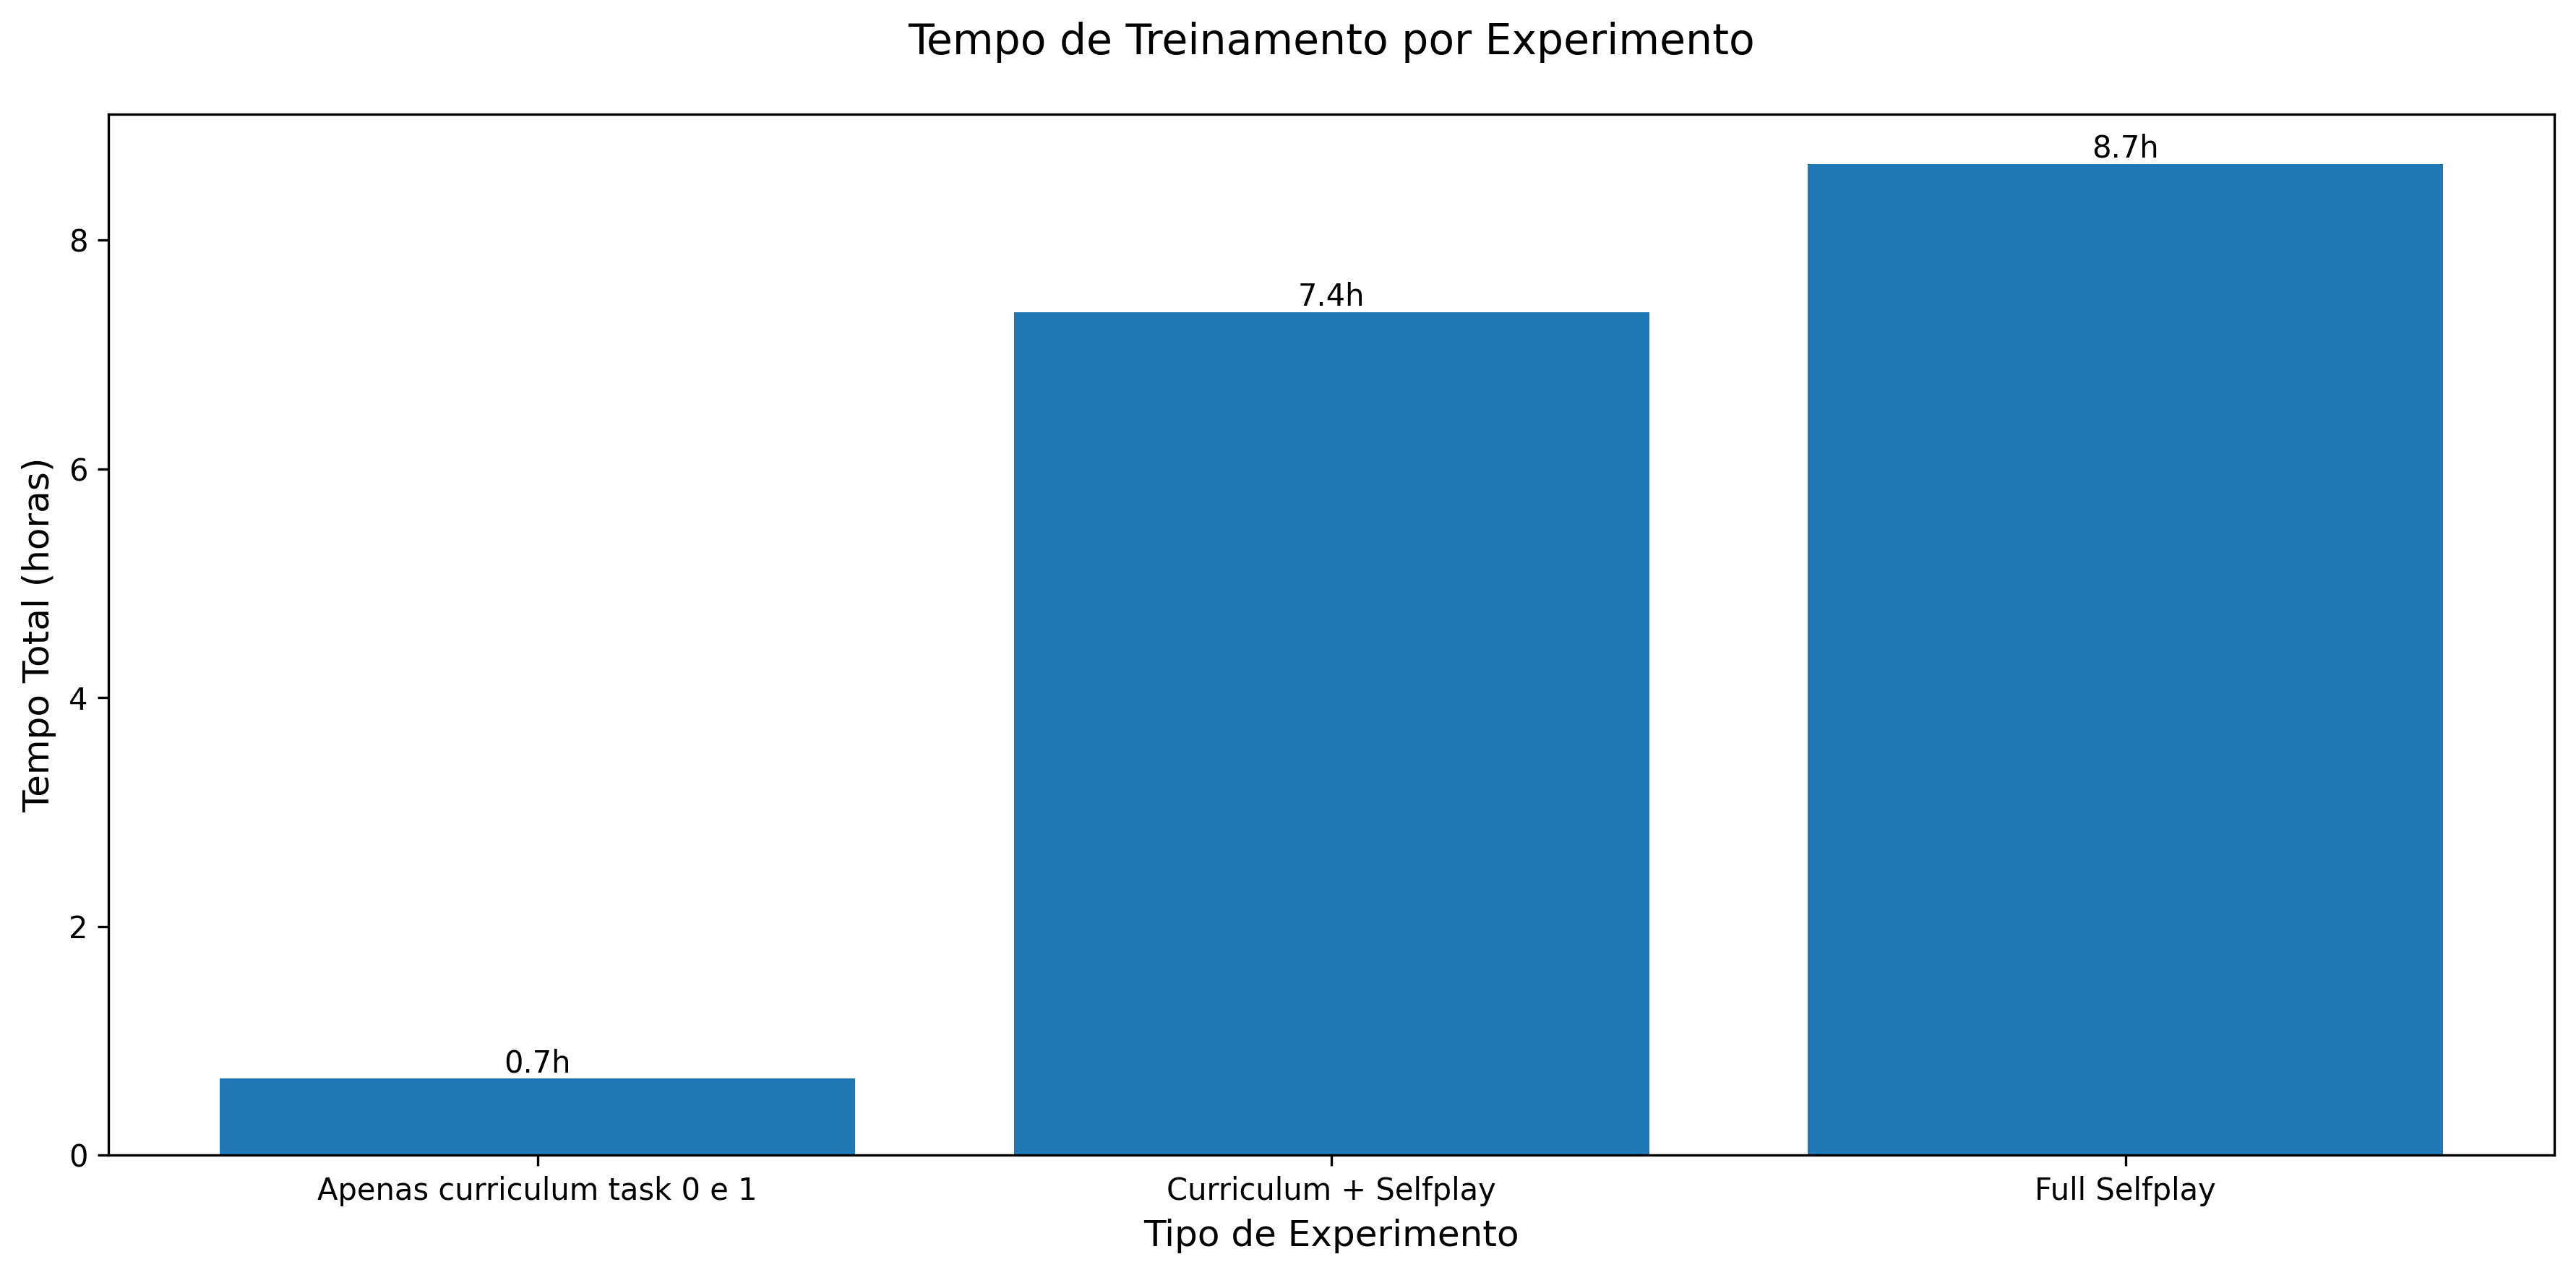
\includegraphics[width=0.9\textwidth]{fig/graficos_trabalho/graficos_experimentos/graficos_tempo_treino/tempo_treinamento.png}
    \caption{Comparação do tempo total de treinamento em horas para cada abordagem experimental}
    \label{fig:tempo_treinamento}
\end{figure}

A análise dos tempos de treinamento revela diferenças significativas entre as abordagens:

\begin{itemize}
    \item \textbf{Apenas curriculum (tasks 0 e 1)}: Aproximadamente 0,4 horas (24 minutos)
    \item \textbf{Curriculum + Self-play}: Aproximadamente 7,4 horas
    \item \textbf{Full Self-play (lado amarelo)}: Aproximadamente 12,1 horas
    \item \textbf{Full Self-play (lado azul)}: Aproximadamente 12,4 horas
\end{itemize}

Estas diferenças nos tempos de treinamento refletem a complexidade e a natureza de cada abordagem. O treinamento exclusivo com curriculum tasks é significativamente mais rápido, pois envolve ambientes mais simples e objetivos bem definidos. A abordagem combinada (curriculum + self-play) apresenta um tempo de treinamento intermediário, demonstrando uma vantagem de eficiência em relação ao self-play tradicional.

É interessante notar que a abordagem de full self-play para ambos os lados (azul e amarelo) exige aproximadamente o mesmo tempo de treinamento, com uma pequena variação que pode ser atribuída a flutuações nas condições de execução. No entanto, ambas requerem aproximadamente 66\% mais tempo que a abordagem combinada (curriculum + self-play).

Esta é uma observação particularmente relevante do ponto de vista prático, pois indica que além de proporcionar resultados superiores (conforme demonstrado nas seções anteriores), a abordagem combinada também oferece uma vantagem significativa em termos de eficiência computacional, reduzindo o tempo necessário para desenvolver agentes com desempenho competitivo.

A maior eficiência da abordagem combinada pode ser atribuída ao fato de que as habilidades fundamentais desenvolvidas durante o curriculum permitem que o agente aproveite melhor a fase de self-play, convergindo mais rapidamente para políticas efetivas.

\section{Análise Comparativa}
\label{sec:analise_comparativa}

Para avaliar a eficácia da abordagem proposta, realizamos uma análise comparativa entre o modelo treinado apenas com self-play (baseline) e o modelo treinado com a combinação de curriculum learning e self-play (modelo proposto). Esta análise abrange diversas métricas relevantes para o domínio do futebol de robôs.

\subsection{Evolução da Recompensa}

A análise da evolução da recompensa média ao longo do treinamento oferece insights valiosos sobre o processo de aprendizagem dos agentes. A Figura \ref{fig:episode_reward} apresenta esta evolução para ambas as abordagens.

\begin{figure}[H]
    \centering
    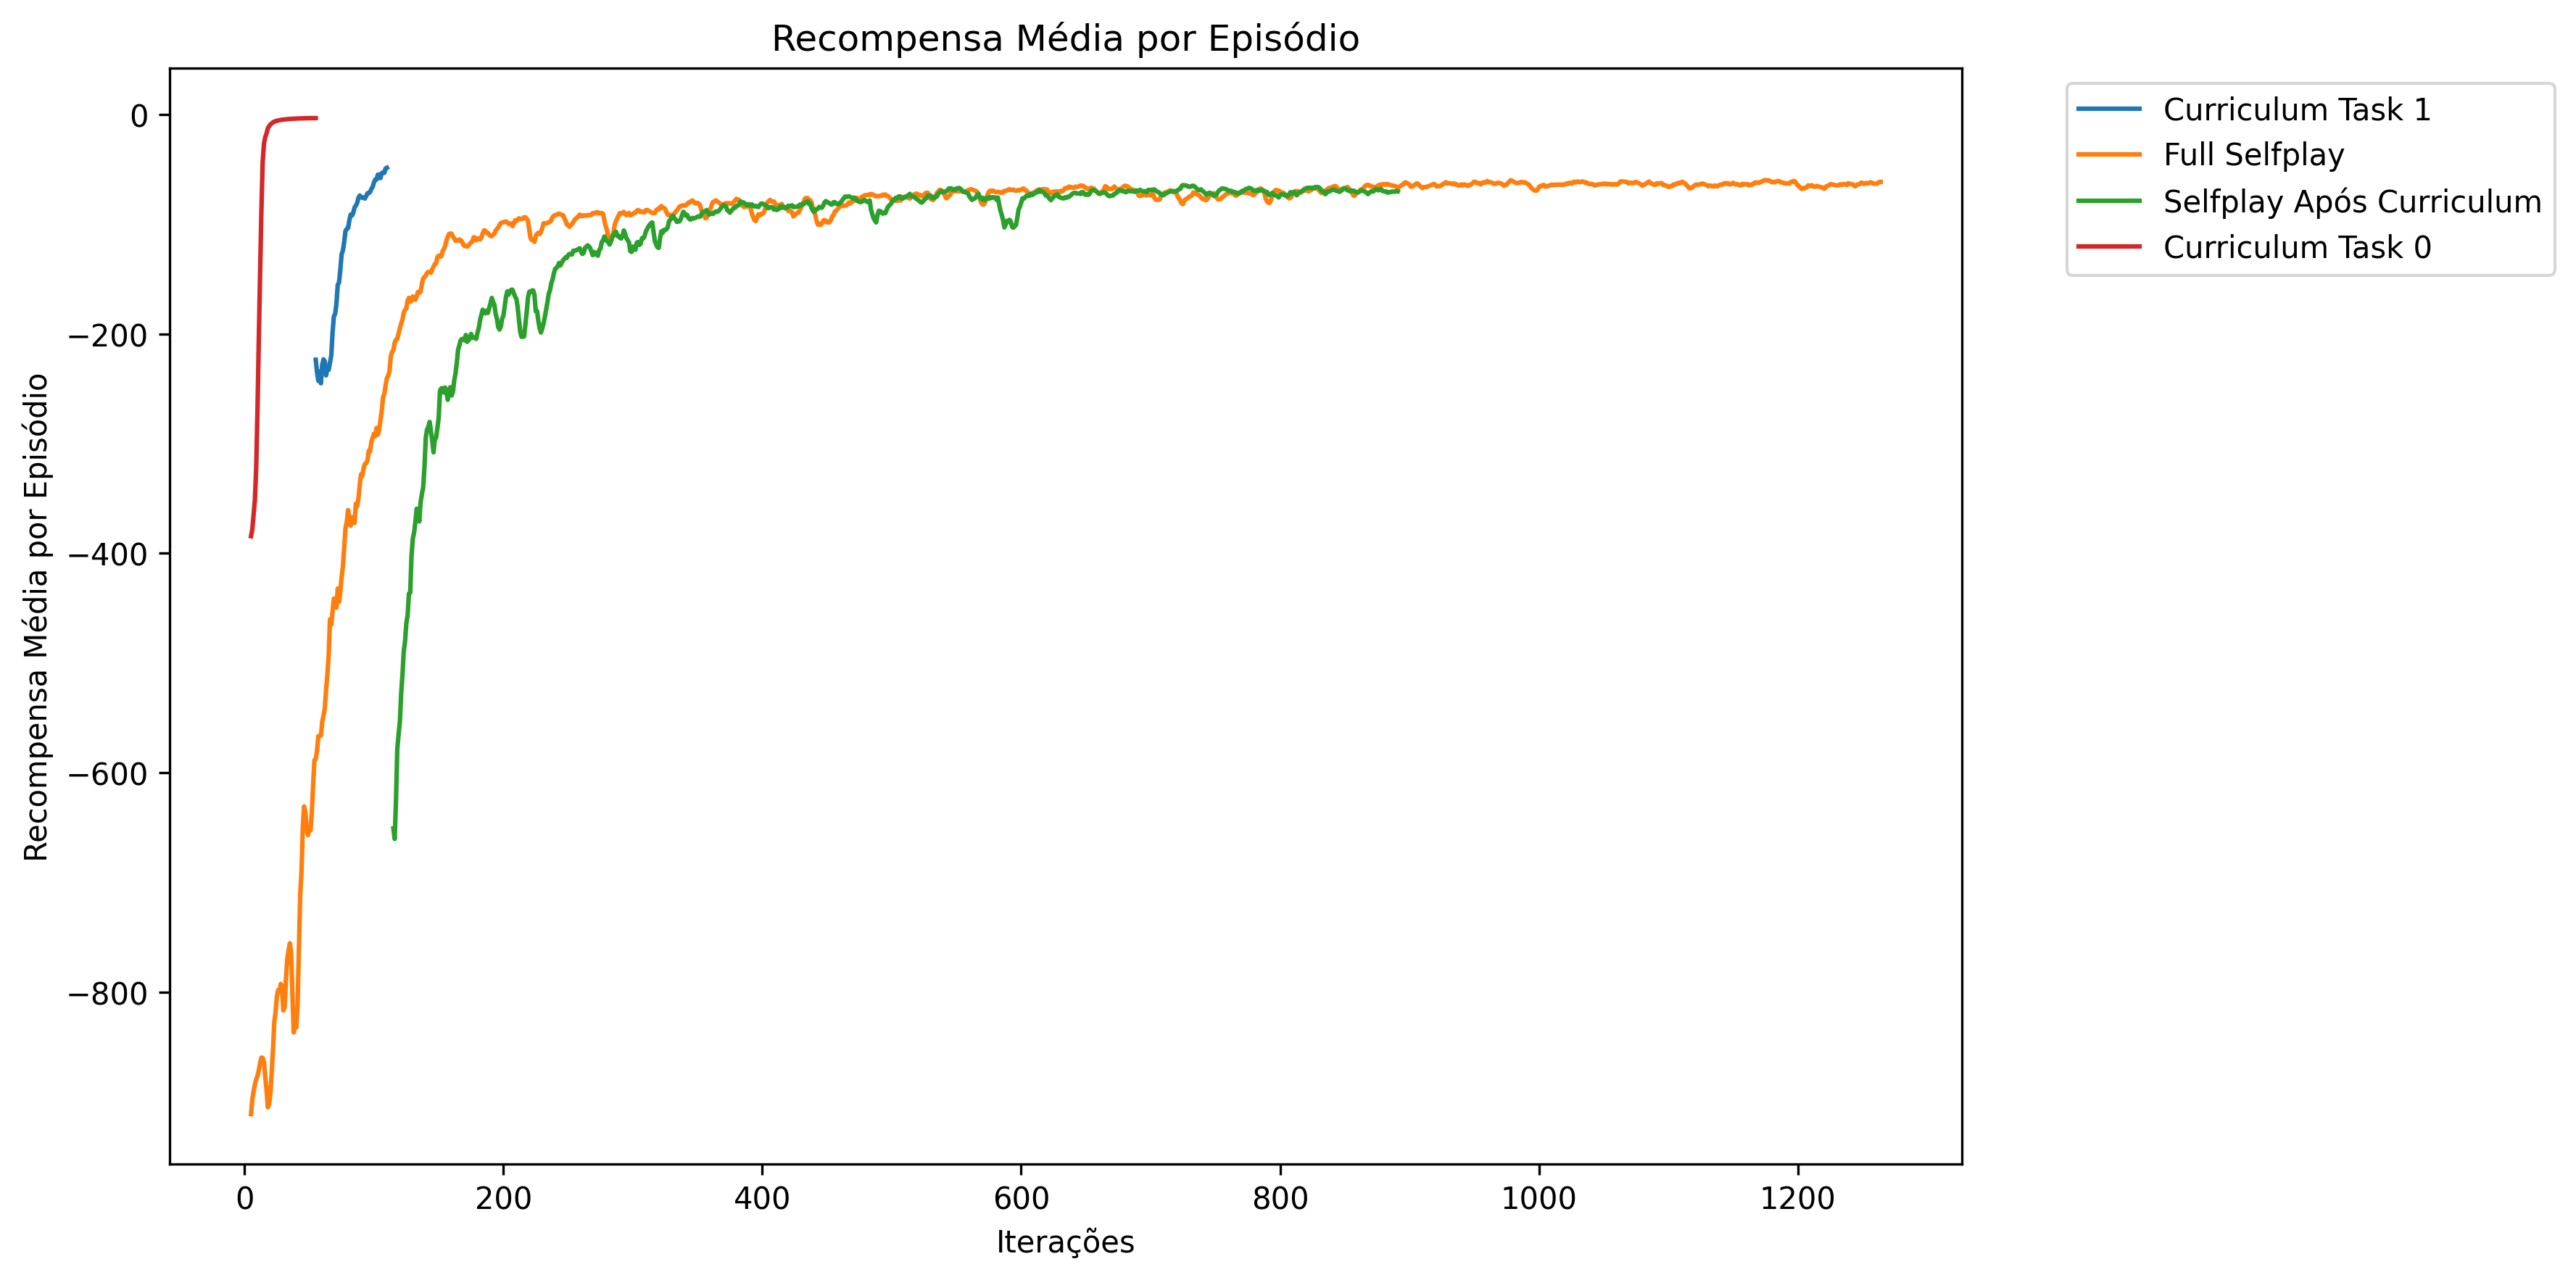
\includegraphics[width=0.8\textwidth]{fig/graficos_trabalho/graficos_experimentos/geral/episode_reward_mean.png}
    \caption{Evolução da recompensa média por episódio ao longo do treinamento}
    \label{fig:episode_reward}
\end{figure}

O gráfico revela que o modelo treinado com curriculum learning apresenta um crescimento mais acelerado da recompensa nas fases iniciais do treinamento. Esta vantagem inicial é atribuída à aprendizagem estruturada de habilidades fundamentais durante os estágios do curriculum. Embora ambas as abordagens apresentem convergência em termos de recompensa acumulada, o modelo proposto atinge níveis equivalentes com menos timesteps de treinamento, sugerindo maior eficiência no processo de aprendizagem.

Nota-se também que o modelo proposto apresenta menor variabilidade na curva de recompensa, indicando maior estabilidade durante o processo de treinamento.

\subsection{Desempenho Ofensivo}

O desempenho ofensivo dos agentes foi avaliado principalmente através da análise da média de gols marcados por episódio. A Figura \ref{fig:goals_blue_comparison} apresenta a evolução desta métrica ao longo do treinamento para ambas as abordagens.

\begin{figure}[H]
    \centering
    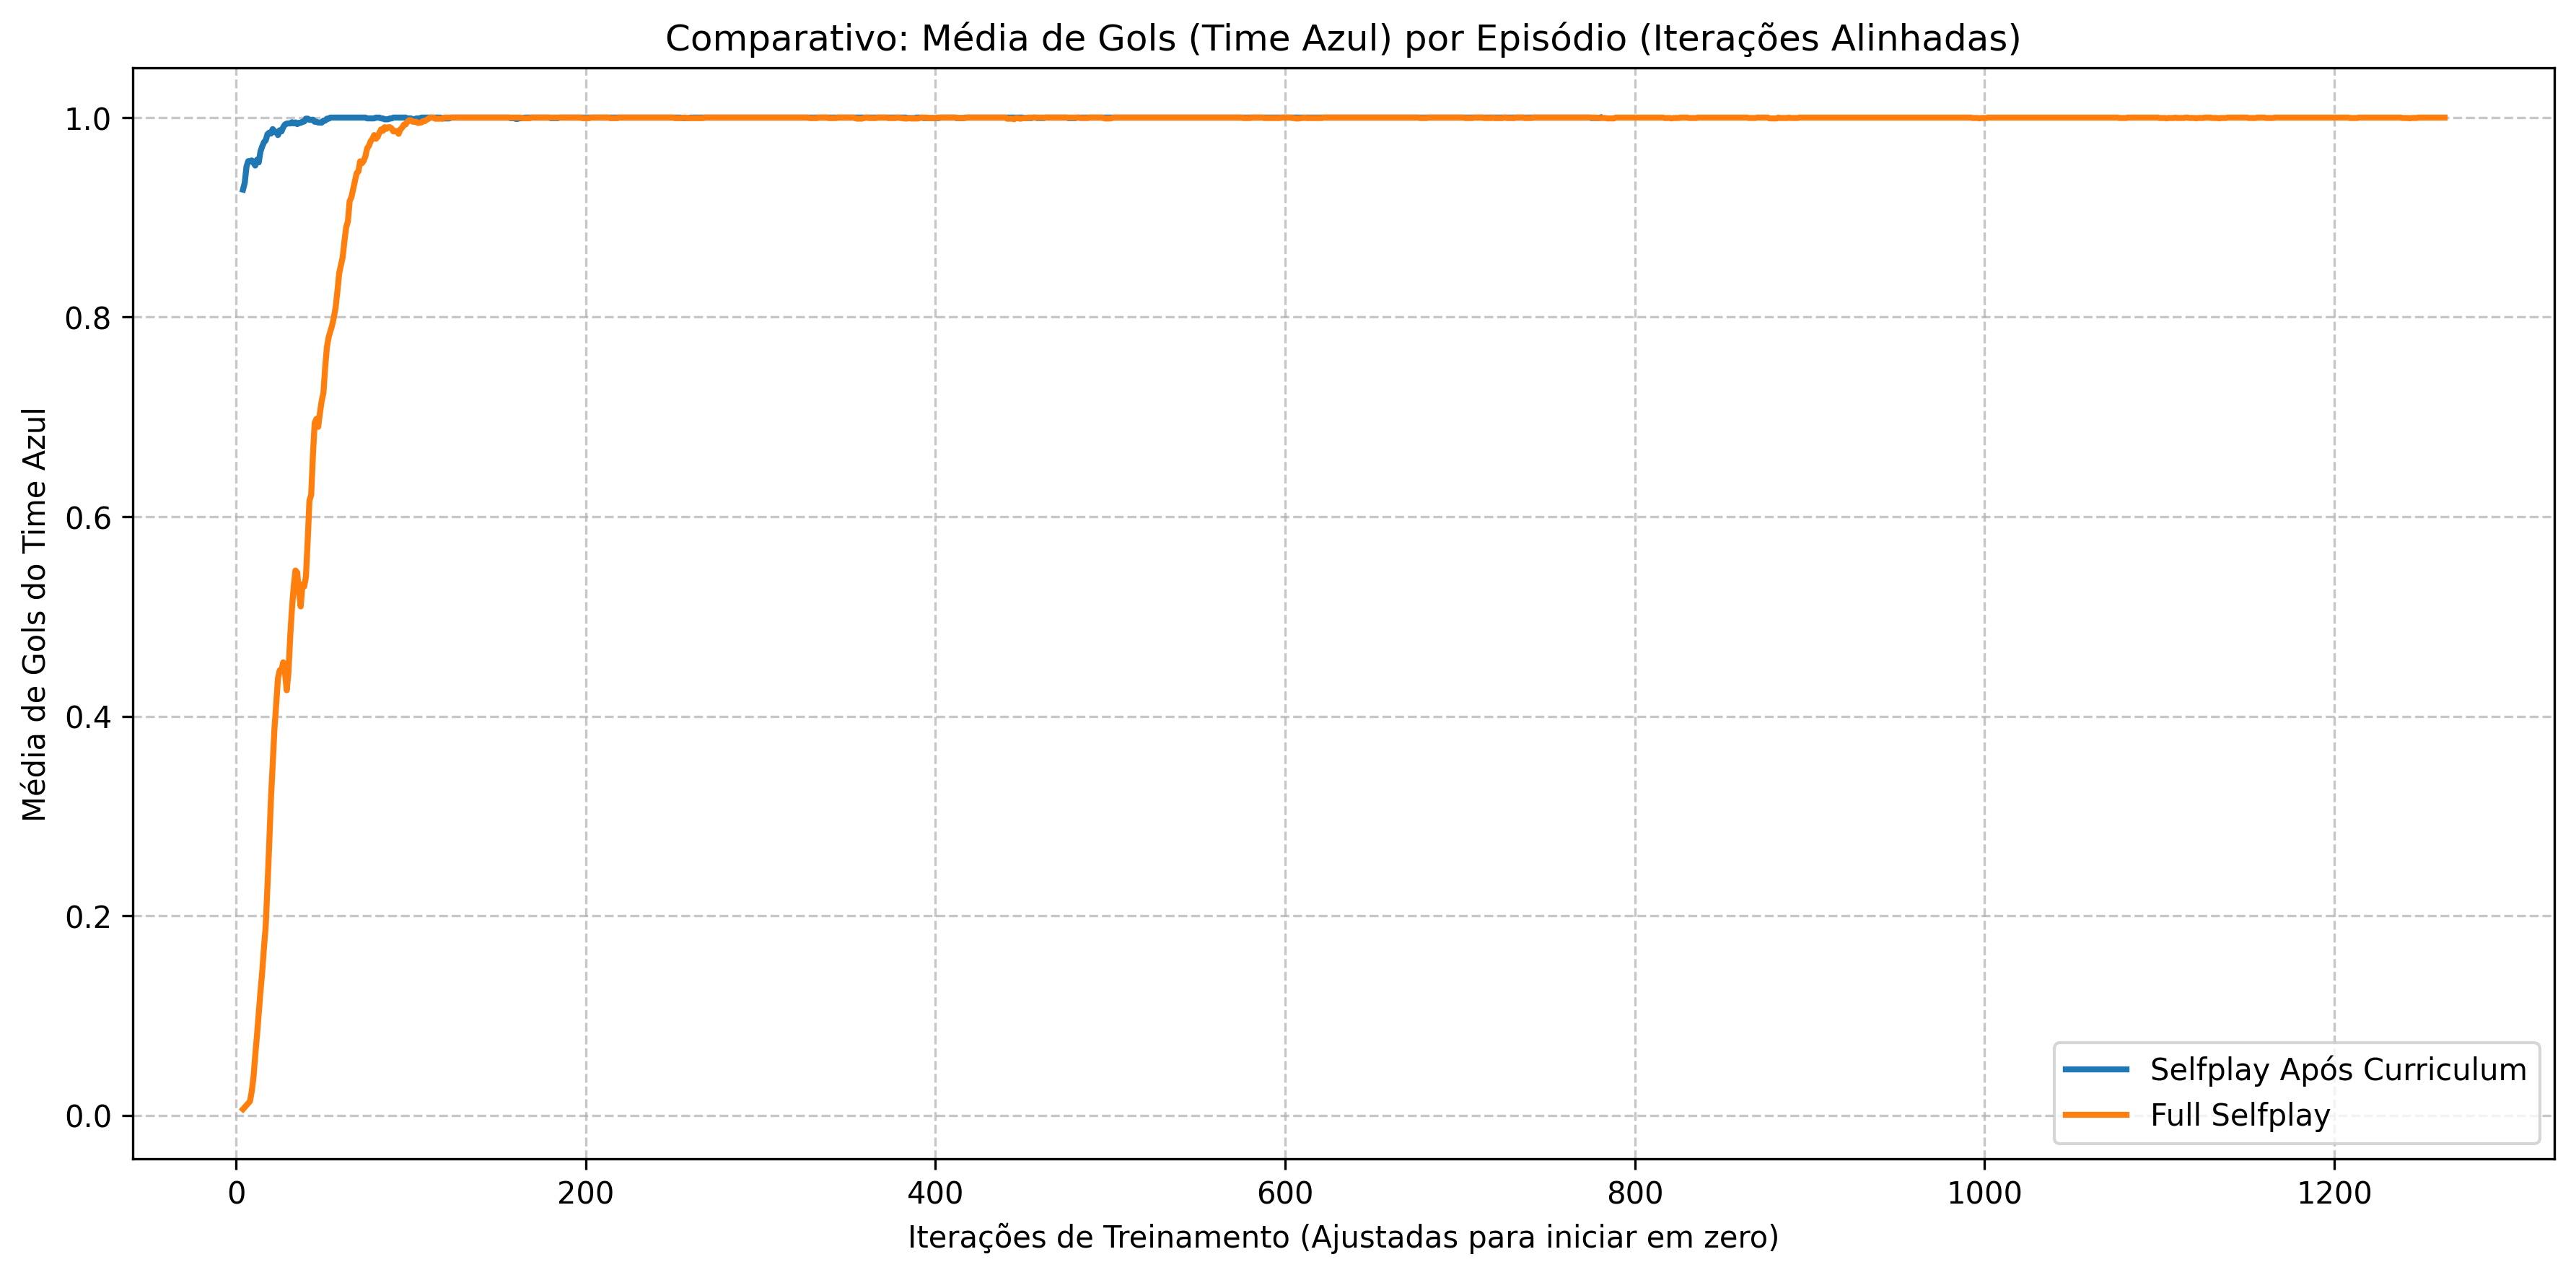
\includegraphics[width=0.95\textwidth]{fig/graficos_trabalho/graficos_experimentos/geral/comparativo_gols_azul_alinhado.png}
    \caption{Comparativo da média de gols do time azul por episódio com iterações alinhadas entre as abordagens Selfplay após Curriculum e Full Selfplay}
    \label{fig:goals_blue_comparison}
\end{figure}

A análise comparativa do gráfico revela padrões interessantes na evolução da capacidade ofensiva dos agentes. Ambas as abordagens apresentam uma progressão crescente na capacidade de marcar gols, atingindo valores próximos a 1 gol por episódio. No entanto, observam-se diferenças significativas no processo de aprendizado:

\begin{itemize}
    \item \textbf{Velocidade de convergência}: O Selfplay após Curriculum (linha azul) atinge o patamar de 1 gol por episódio muito mais rapidamente, convergindo em aproximadamente 100 iterações, enquanto o Full Selfplay (linha laranja) requer cerca de 150 iterações para alcançar o mesmo desempenho.
    
    \item \textbf{Fase inicial}: Nas primeiras iterações, o Selfplay após Curriculum já começa com uma vantagem significativa, demonstrando que as habilidades adquiridas durante a fase de curriculum proporcionam um ponto de partida mais avançado para o desenvolvimento ofensivo.
    
    \item \textbf{Estabilidade}: Ambas as abordagens eventualmente atingem estabilidade na média de gols, mas o Selfplay após Curriculum apresenta menor variabilidade na fase de convergência, indicando um processo de aprendizado mais consistente.
\end{itemize}

Esta comparação com iterações alinhadas evidencia de forma clara uma vantagem significativa da abordagem proposta: ao iniciar o self-play com agentes já treinados em tarefas fundamentais através do curriculum, obtém-se uma aceleração substancial no desenvolvimento de capacidades ofensivas eficazes. Esta característica é particularmente valiosa em cenários com restrições de tempo computacional, onde a convergência mais rápida para políticas de alta qualidade representa uma vantagem considerável.

\subsection{Eficiência e Continuidade do Jogo}

Um aspecto diferencial da abordagem proposta é a melhoria significativa nas métricas relacionadas à continuidade do jogo, que refletem a capacidade dos agentes de manter a bola em jogo por períodos mais longos. A Figura \ref{fig:total_resets} apresenta a evolução do número médio de resets por episódio.

\begin{figure}[H]
    \centering
    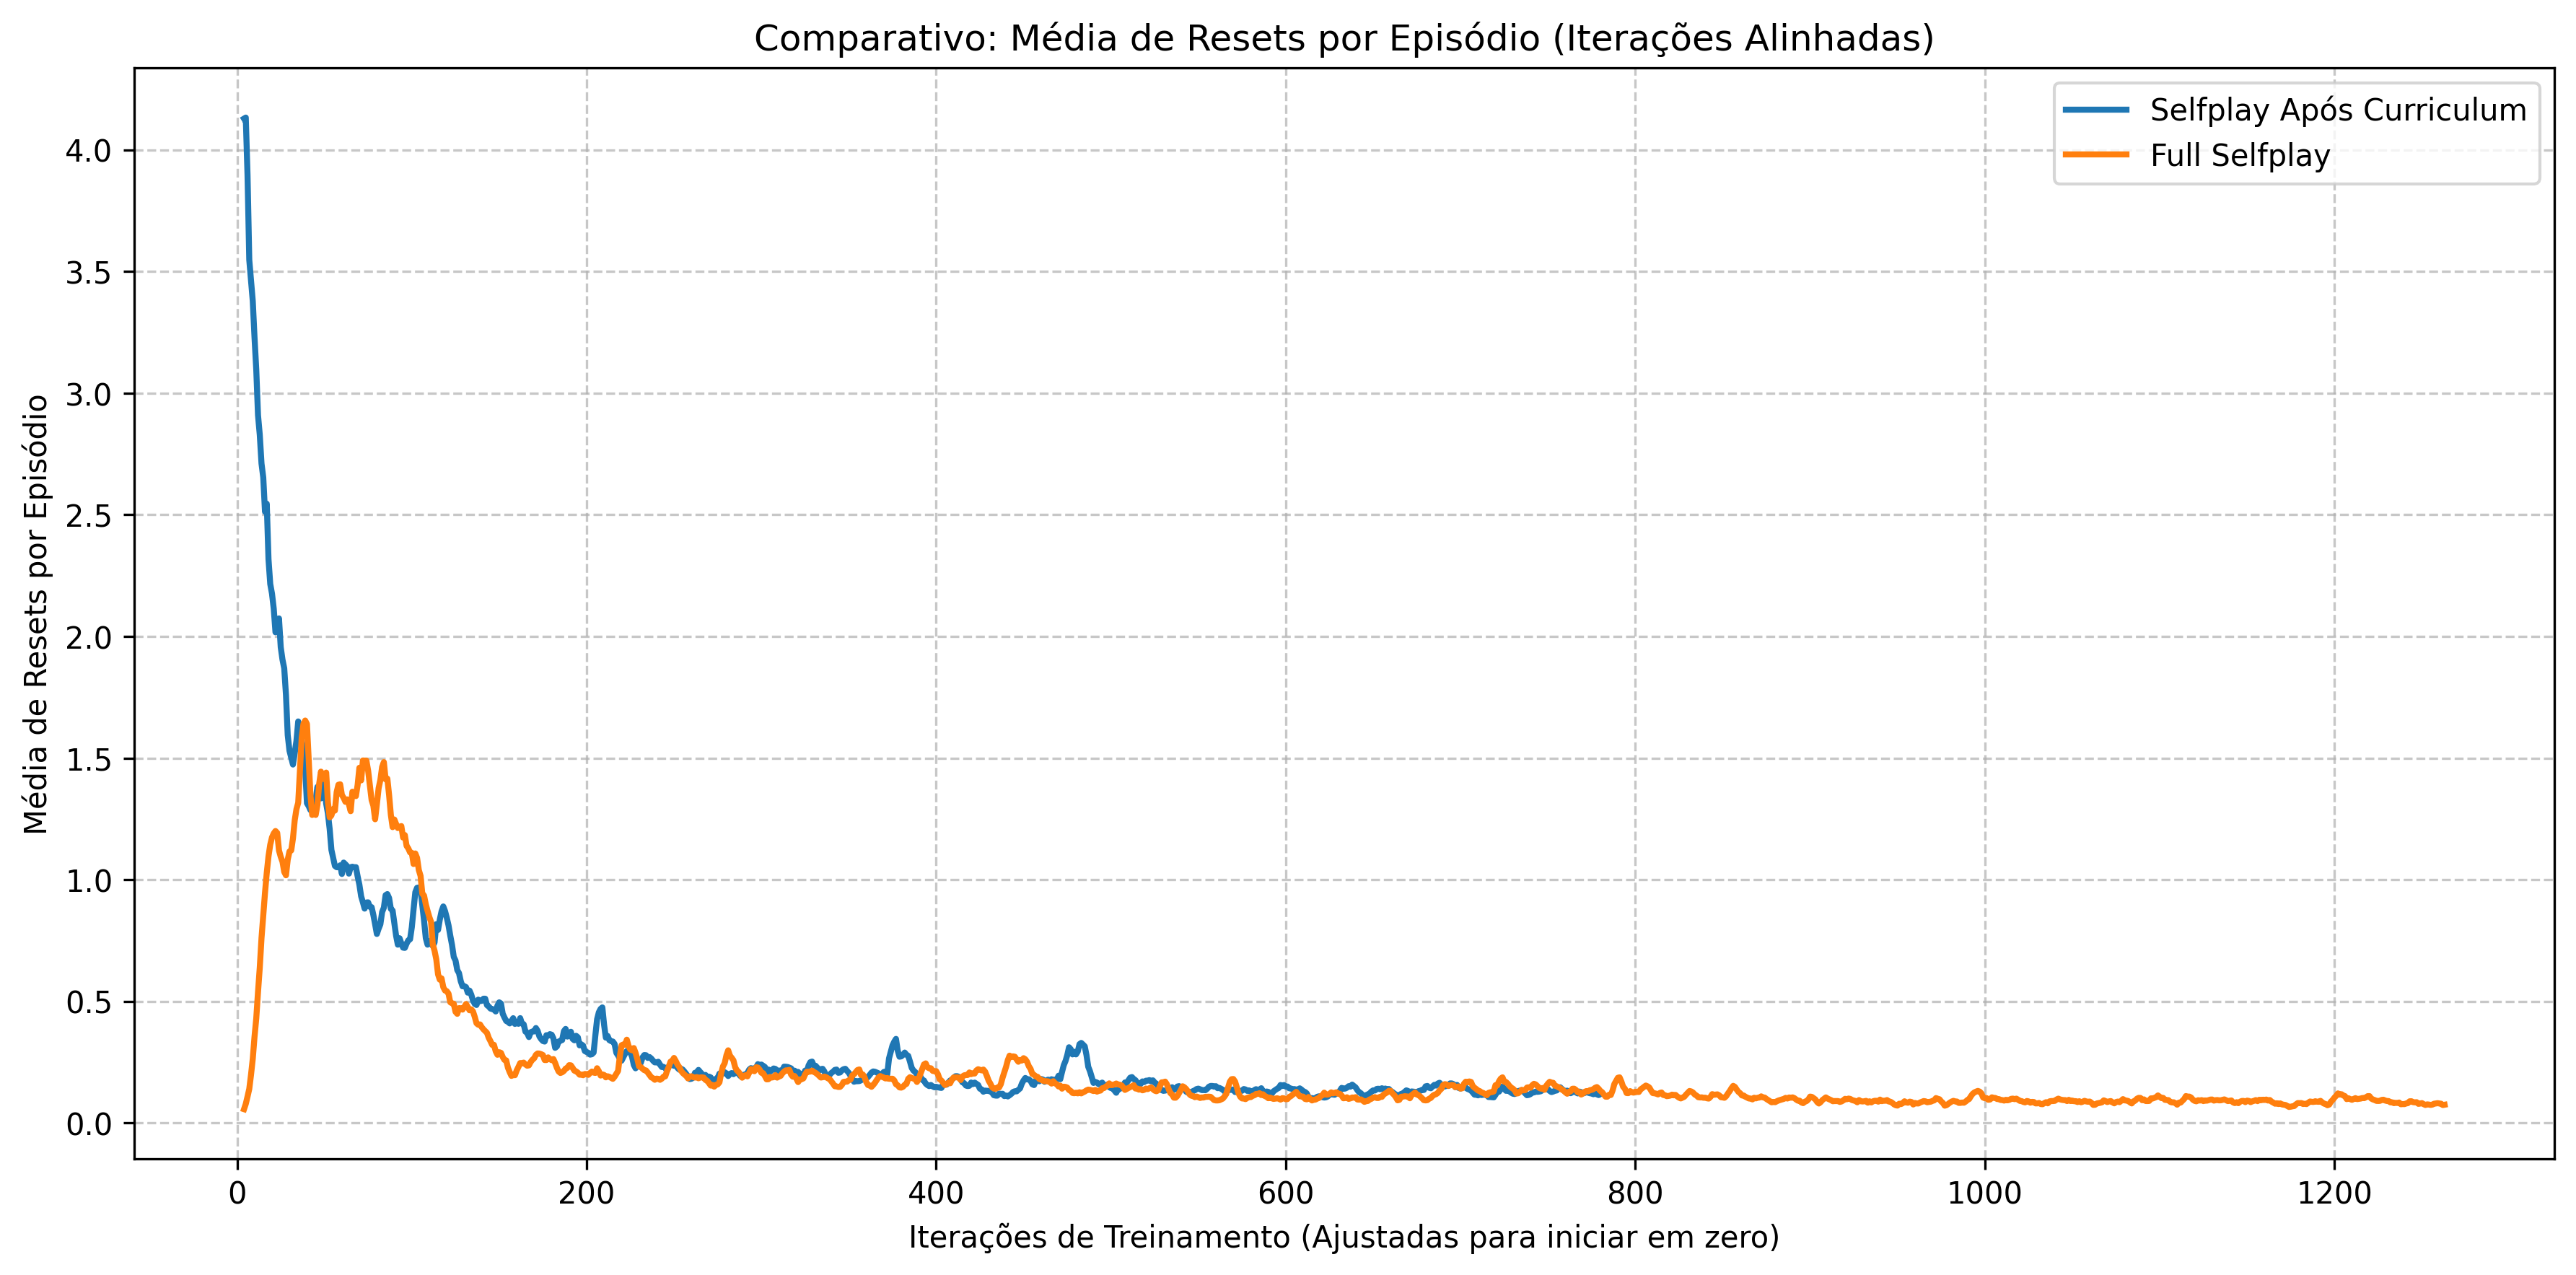
\includegraphics[width=0.95\textwidth]{fig/graficos_trabalho/graficos_experimentos/geral/comparativo_resets_episodio_alinhado.png}
    \caption{Comparativo da média de resets por episódio com iterações alinhadas entre as abordagens Selfplay após Curriculum e Full Selfplay}
    \label{fig:total_resets}
\end{figure}

A análise do gráfico revela diferenças significativas nos padrões de aprendizado relacionados à continuidade do jogo. Inicialmente, o Selfplay após Curriculum (linha azul) apresenta um pico maior de resets por episódio, mas rapidamente consegue reduzir esse número. O Full Selfplay (linha laranja) mostra um comportamento diferente, com um aumento gradual seguido por uma redução mais lenta.

Após aproximadamente 200 iterações, ambas as abordagens convergem para valores similares, com ligeira vantagem para o Full Selfplay nas iterações finais. No entanto, é notável que o Selfplay após Curriculum consegue reduzir o número de resets de forma mais rápida nas fases iniciais do treinamento, evidenciando a transferência positiva das habilidades adquiridas durante o curriculum.

Complementarmente, a análise do tempo médio entre resets (Figura \ref{fig:time_between_resets}) reforça esta observação sobre os diferentes padrões de aprendizado.

\begin{figure}[H]
    \centering
    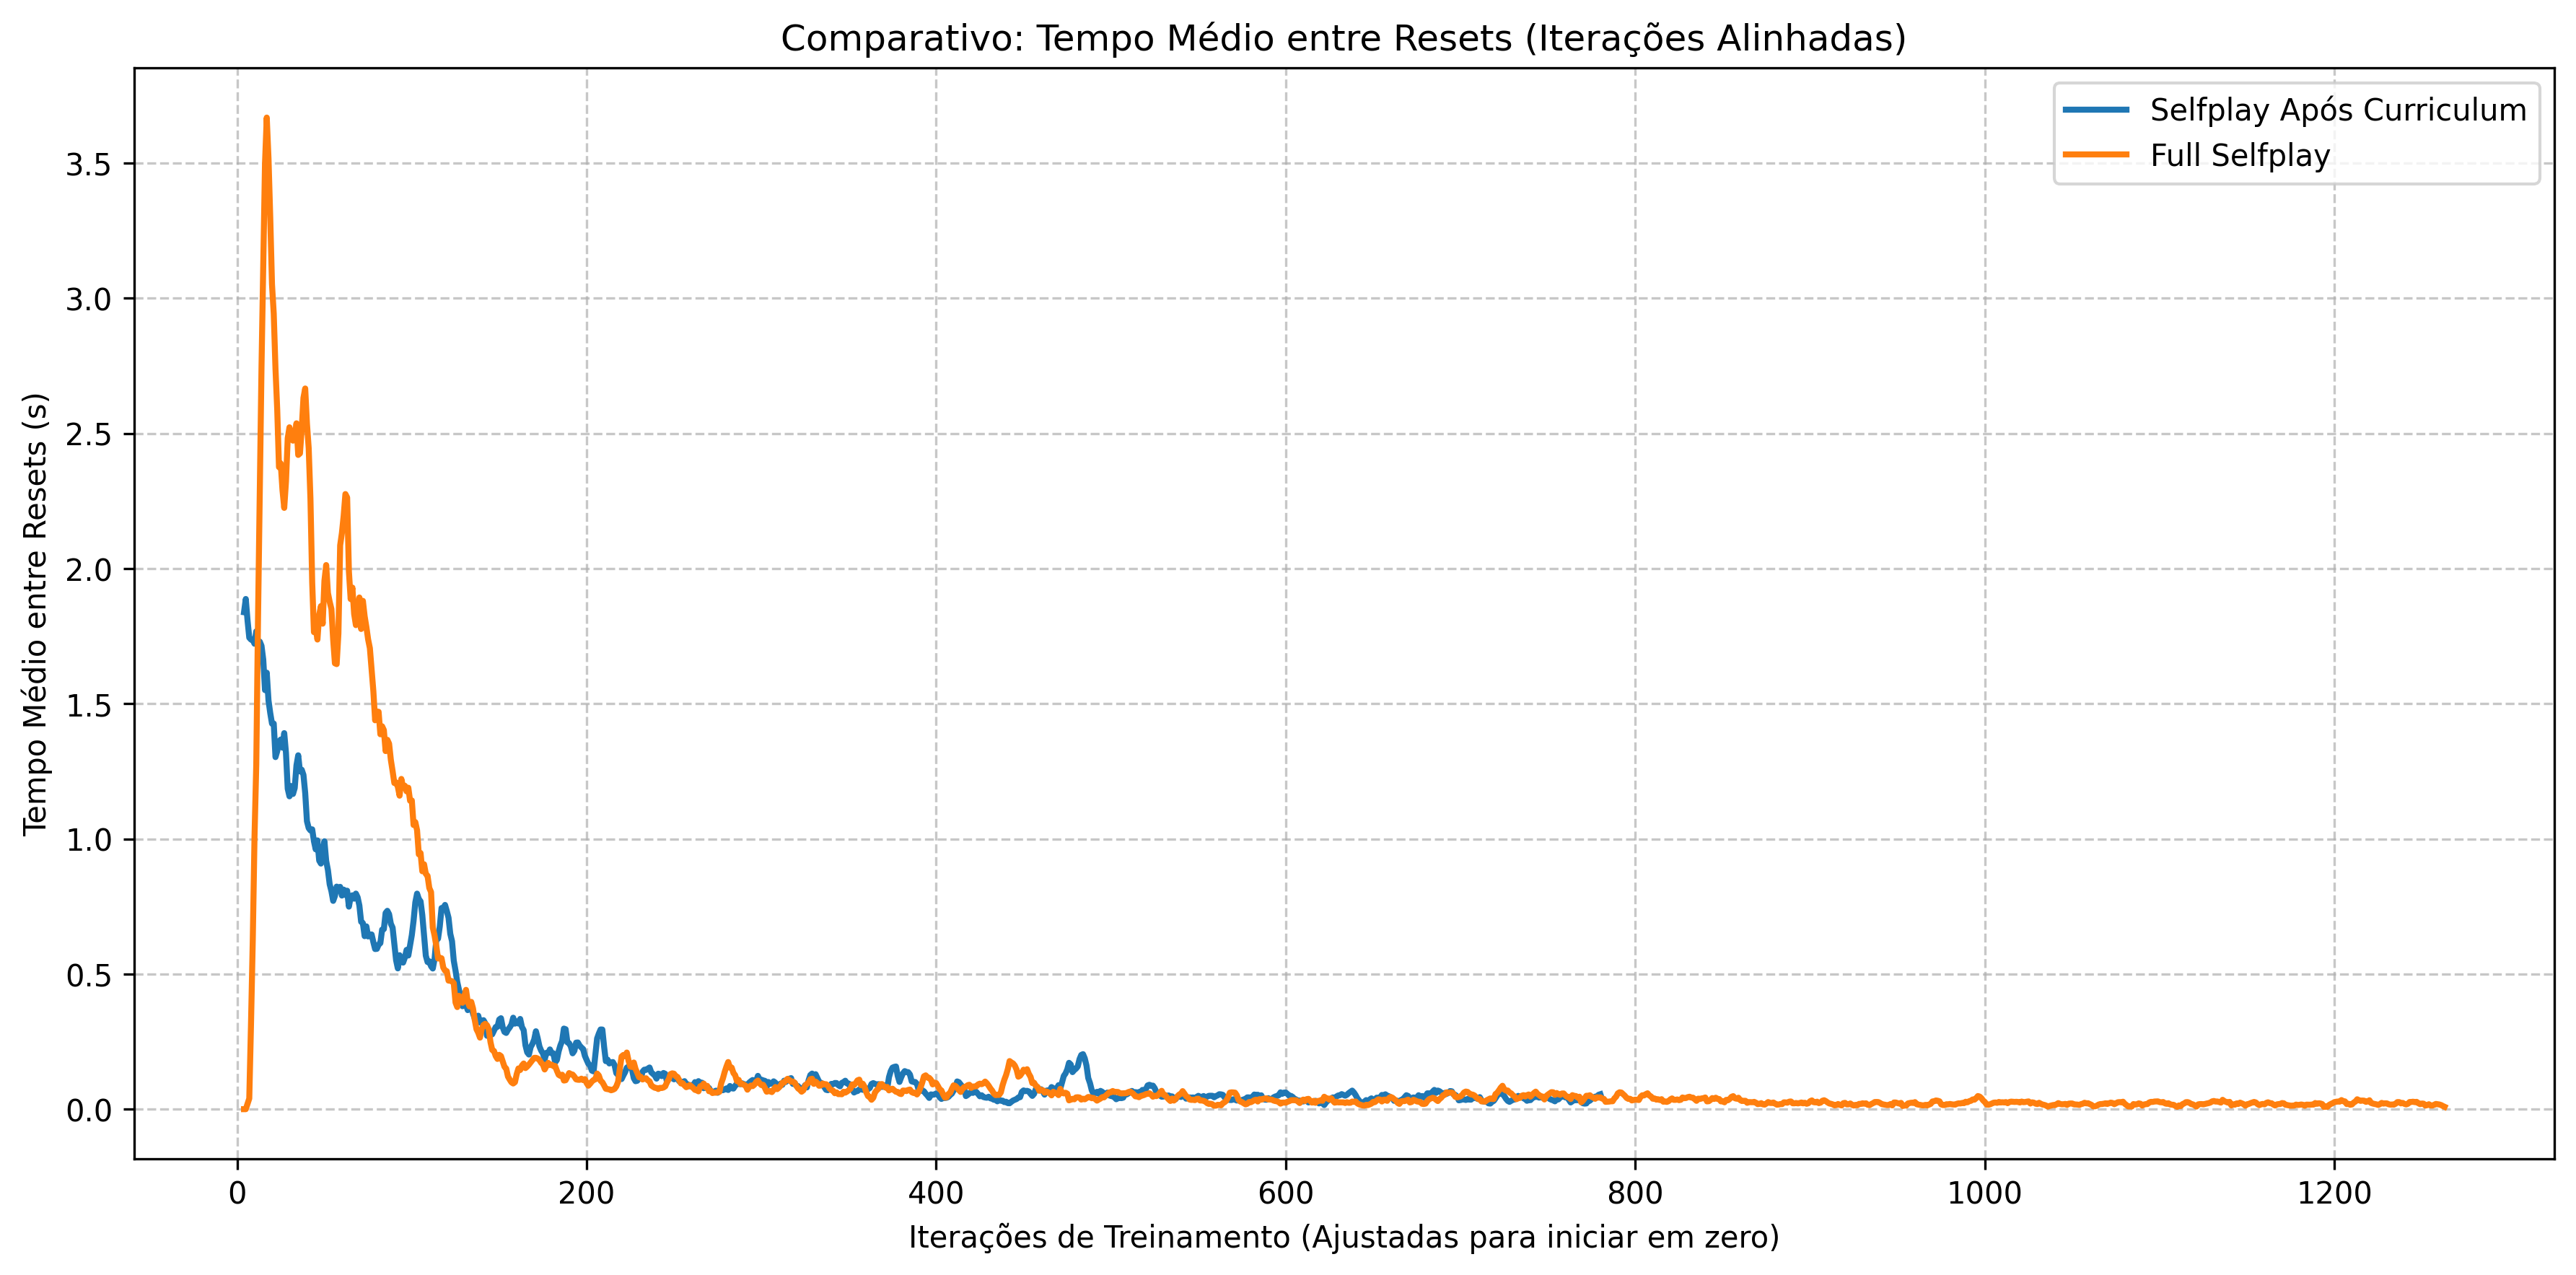
\includegraphics[width=0.95\textwidth]{fig/graficos_trabalho/graficos_experimentos/geral/comparativo_tempo_entre_resets_alinhado.png}
    \caption{Comparativo do tempo médio entre resets com iterações alinhadas entre as abordagens Selfplay após Curriculum e Full Selfplay}
    \label{fig:time_between_resets}
\end{figure}

O gráfico de tempo médio entre resets mostra tendências inversamente relacionadas ao número de resets, como esperado. Interessantemente, enquanto o Full Selfplay (linha laranja) apresenta inicialmente picos mais altos, indicando períodos mais longos sem interrupções, sua curva de aprendizado para esta métrica é mais lenta e volátil.

O Selfplay após Curriculum demonstra uma curva de aprendizado mais estável, sem os picos extremos, mas com uma progressão mais consistente. Após a iteração 200, ambas as abordagens convergem para valores similares.

Esta análise comparativa com iterações alinhadas demonstra que, embora ambas as abordagens eventualmente atinjam desempenhos similares em termos de continuidade do jogo em suas fases finais, o Selfplay após Curriculum oferece um processo de aprendizado mais eficiente e estável, especialmente durante as fases iniciais e intermediárias do treinamento.

\subsection{Duração dos Episódios}

A análise da duração média dos episódios ao longo do treinamento (Figura \ref{fig:episode_len}) revela padrões interessantes sobre a evolução das estratégias desenvolvidas pelos agentes.

\begin{figure}[H]
    \centering
    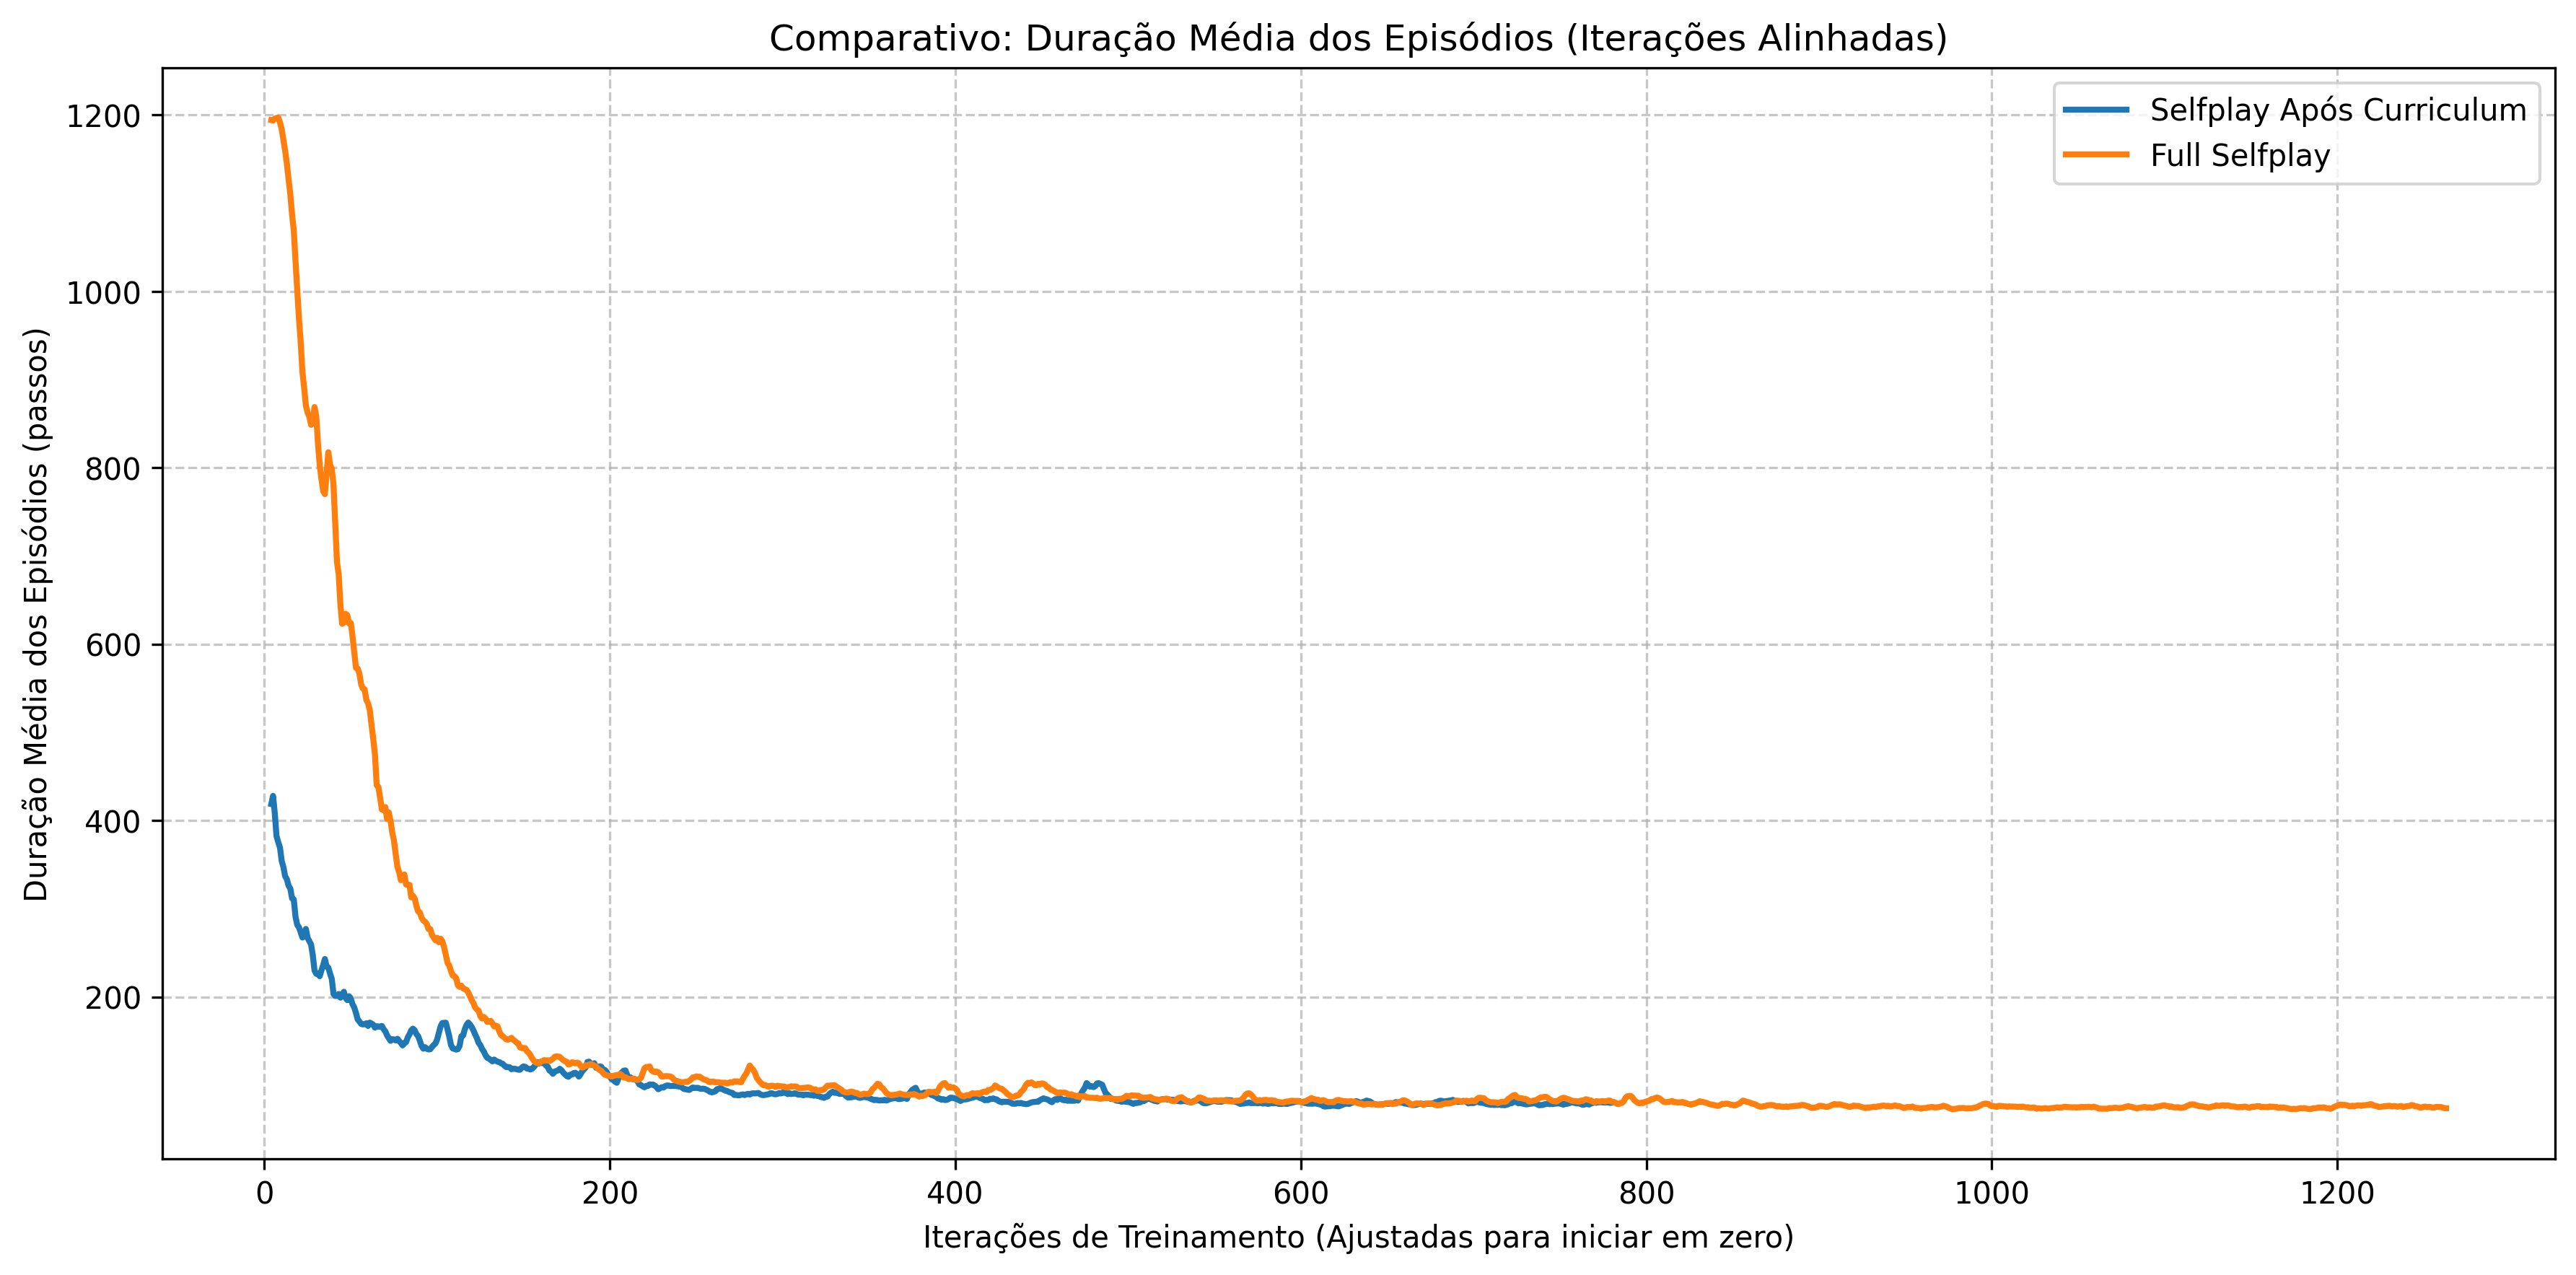
\includegraphics[width=0.95\textwidth]{fig/graficos_trabalho/graficos_experimentos/geral/comparativo_duracao_episodios_alinhado.png}
    \caption{Comparativo da duração média dos episódios com iterações alinhadas entre as abordagens Selfplay após Curriculum e Full Selfplay}
    \label{fig:episode_len}
\end{figure}

A análise do gráfico revela diferenças marcantes no comportamento dos agentes em relação à duração dos episódios. O Full Selfplay (linha laranja) inicia com episódios significativamente mais longos, atingindo aproximadamente 1200 passos nas primeiras iterações, enquanto o Selfplay após Curriculum (linha azul) começa com episódios bem mais curtos, em torno de 400 passos. Esta diferença inicial demonstra que as habilidades adquiridas durante as fases de curriculum proporcionam um ponto de partida mais eficiente, permitindo aos agentes atingir seus objetivos em menos passos desde o início.

Ao longo do treinamento, ambas as abordagens apresentam uma redução gradual na duração dos episódios, convergindo para valores similares após aproximadamente 200 iterações, quando estabilizam em torno de 100 passos por episódio. É notável, porém, que o Selfplay após Curriculum apresenta uma curva de aprendizado mais suave e consistente, sem as oscilações pronunciadas observadas no Full Selfplay, indicando um processo de aprendizagem mais estável. Nas iterações finais, ambas as abordagens mantêm desempenho similar, mas o caminho percorrido pelo Selfplay após Curriculum para atingir este patamar demonstra maior eficiência, especialmente nas fases críticas iniciais e intermediárias do treinamento.

\subsection{Avaliação por Torneios}

Para uma avaliação mais abrangente e realista do desempenho dos modelos treinados, foram realizados torneios controlados com 500 partidas utilizando o sistema Arena Serra Dourada, implementado especificamente para este trabalho. Este sistema permitiu a realização de partidas completas com 10 minutos de duração entre agentes treinados por diferentes métodos.

A Figura \ref{fig:comparacao_vitorias} apresenta a comparação do número de vitórias obtidas por cada abordagem nos torneios realizados.

\begin{figure}[H]
    \centering
    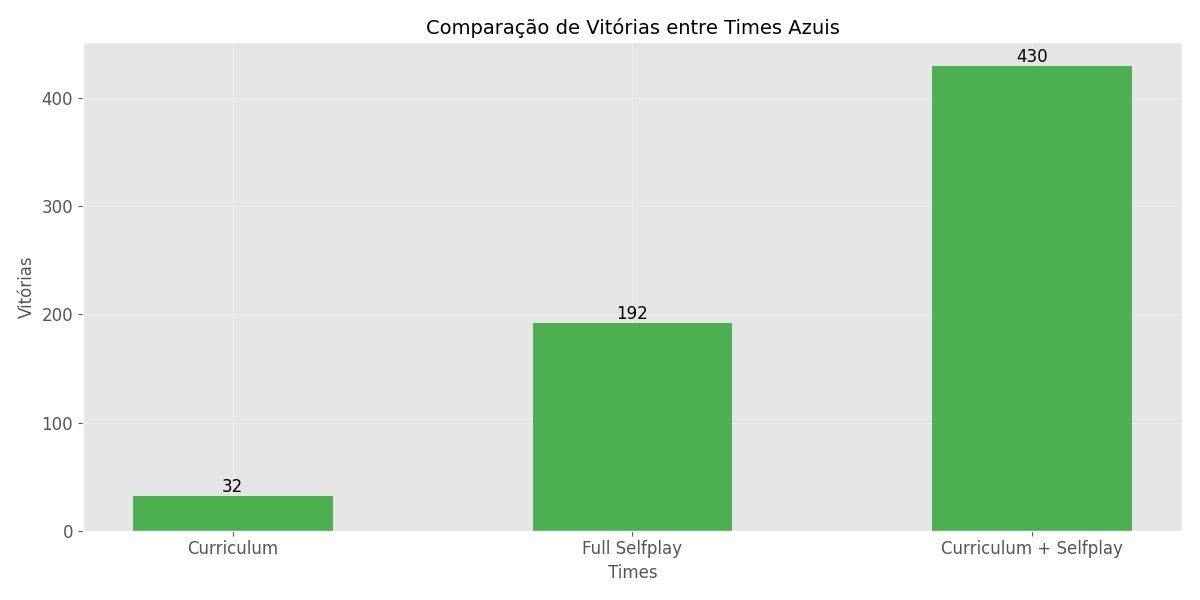
\includegraphics[width=0.8\textwidth]{fig/graficos_trabalho/graficos_torneios/geral/comparacao_vitorias.png}
    \caption{Comparação do número de vitórias por abordagem nos torneios com 500 partidas}
    \label{fig:comparacao_vitorias}
\end{figure}

Os resultados evidenciam a superioridade do modelo treinado com a combinação de curriculum learning e self-play, que obteve 430 vitórias (86\%) em comparação com 192 vitórias (38,4\%) do modelo full self-play tradicional e apenas 32 vitórias (6,4\%) do modelo treinado somente com curriculum learning. Esta diferença na taxa de vitória é estatisticamente significativa e demonstra o benefício substancial da abordagem híbrida proposta.

É interessante notar que o modelo treinado apenas com curriculum learning obteve o menor número de vitórias, mas também apresentou o maior número de empates (468, correspondendo a 93,6\% dos jogos), o que sugere uma estratégia mais defensiva e conservadora. Por outro lado, o modelo combinado (curriculum + self-play) não apenas venceu mais partidas, mas também registrou o menor número de empates (70, apenas 14\% dos jogos), indicando uma abordagem mais assertiva e eficaz.

\subsection{Análise de Gols nos Torneios}

Além da taxa de vitória, analisamos também o desempenho ofensivo e defensivo dos modelos nos torneios realizados, conforme ilustrado nas Figuras \ref{fig:comparacao_gols_feitos} e \ref{fig:comparacao_gols_sofridos}.

\begin{figure}[H]
    \centering
    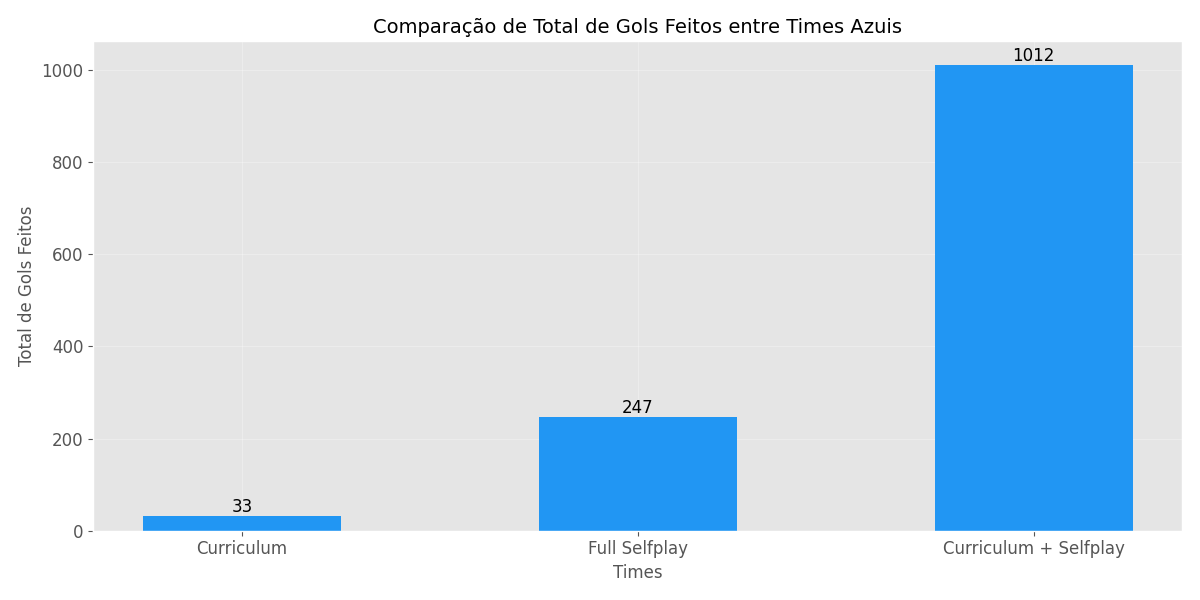
\includegraphics[width=0.8\textwidth]{fig/graficos_trabalho/graficos_torneios/geral/comparacao_gols_feitos.png}
    \caption{Comparação do número total de gols marcados por abordagem nos torneios}
    \label{fig:comparacao_gols_feitos}
\end{figure}

\begin{figure}[H]
    \centering
    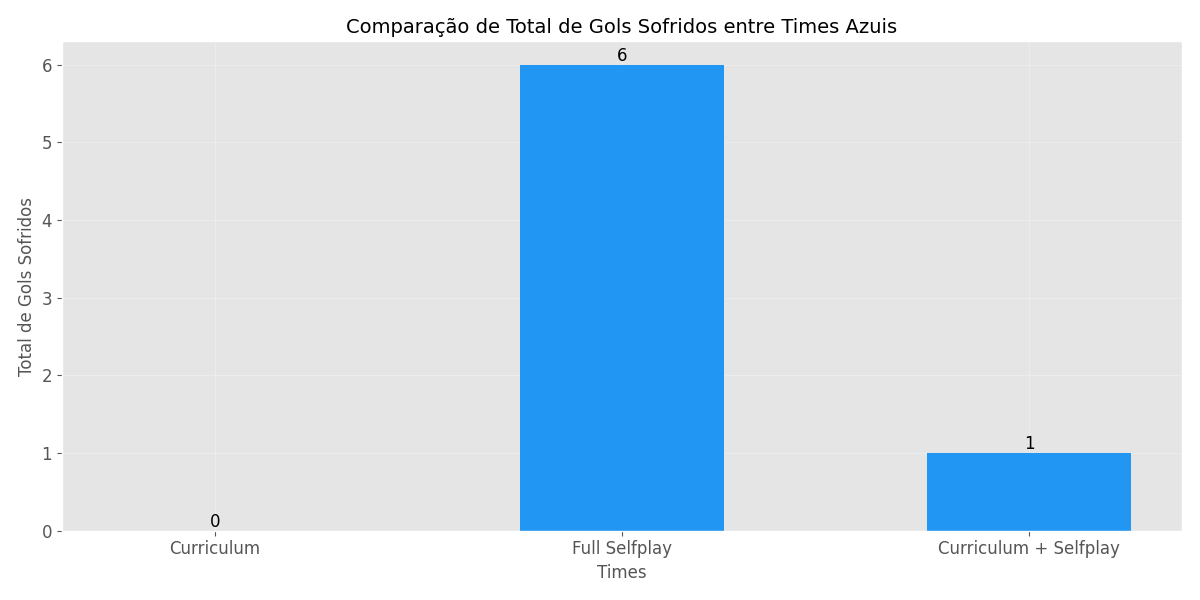
\includegraphics[width=0.8\textwidth]{fig/graficos_trabalho/graficos_torneios/geral/comparacao_gols_sofridos.png}
    \caption{Comparação do número total de gols sofridos por abordagem nos torneios}
    \label{fig:comparacao_gols_sofridos}
\end{figure}

Os dados revelam diferenças significativas no desempenho ofensivo e defensivo entre as três abordagens. O modelo combinado (curriculum + self-play) apresentou uma capacidade ofensiva superior, marcando um total de 1.012 gols durante o torneio, o que corresponde a uma média de 2,024 gols por partida. Em contraste, o modelo treinado exclusivamente com self-play marcou 247 gols (média de 0,494 por partida), enquanto o modelo que utilizou apenas curriculum learning obteve apenas 33 gols (média de 0,066 por partida).

Do ponto de vista defensivo, todos os modelos demonstraram robustez considerável, mas com diferenças notáveis. O modelo treinado apenas com curriculum learning não sofreu nenhum gol durante todo o torneio, demonstrando uma excelente capacidade defensiva que compensa parcialmente sua limitada capacidade ofensiva. O modelo combinado sofreu apenas 1 gol em 500 partidas (média de 0,002 por partida), enquanto o modelo full self-play sofreu 6 gols (média de 0,012 por partida).

Estes resultados sugerem que o curriculum learning contribui significativamente para o desenvolvimento de habilidades defensivas sólidas, enquanto a combinação com self-play permite que essas habilidades sejam complementadas por estratégias ofensivas eficazes. A abordagem combinada consegue, portanto, obter o melhor dos dois mundos: a solidez defensiva do curriculum learning e a agressividade ofensiva desenvolvida durante o self-play competitivo.

\subsection{Análise de Trade-offs entre Abordagens}

Uma observação importante que emerge da análise dos dados dos torneios é o claro trade-off entre as diferentes abordagens de treinamento. A Tabela \ref{tab:comparacao_abordagens} resume as principais métricas para cada abordagem, facilitando a visualização destes trade-offs.

\begin{table}[H]
    \centering
    \begin{tabular}{|c|c|c|c|}
        \hline
        \textbf{Métrica} & \textbf{Curriculum} & \textbf{Full Self-play} & \textbf{Curriculum + Self-play} \\
        \hline
        Vitórias & 32 (6,4\%) & 192 (38,4\%) & 430 (86\%) \\
        \hline
        Empates & 468 (93,6\%) & 307 (61,4\%) & 70 (14\%) \\
        \hline
        Derrotas & 0 (0\%) & 1 (0,2\%) & 0 (0\%) \\
        \hline
        Gols marcados & 33 & 247 & 1.012 \\
        \hline
        Gols sofridos & 0 & 6 & 1 \\
        \hline
        Média de gols/partida & 0,066 & 0,494 & 2,024 \\
        \hline
    \end{tabular}
    \caption{Comparação entre as três abordagens de treinamento nos torneios com 500 partidas}
    \label{tab:comparacao_abordagens}
\end{table}

A análise desta tabela revela padrões claros:

\begin{enumerate}
    \item \textbf{Curriculum Learning puro}: Desenvolve agentes extremamente defensivos e conservadores, com excelente capacidade de evitar gols (nenhum gol sofrido), mas limitada capacidade ofensiva (apenas 0,066 gols por partida). Esta abordagem resulta em muitos empates (93,6\%) e poucas vitórias (6,4\%).
    
    \item \textbf{Full Self-play}: Produz agentes com um perfil mais equilibrado, capazes de marcar gols com frequência moderada (0,494 por partida) e manter uma defesa relativamente sólida. Esta abordagem leva a um número significativo de vitórias (38,4\%), mas também muitos empates (61,4\%).
    
    \item \textbf{Curriculum + Self-play}: Representa o melhor equilíbrio entre capacidades ofensivas e defensivas, com uma notável capacidade de marcar gols (2,024 por partida) enquanto mantém uma defesa quase impenetrável (apenas 1 gol sofrido em 500 partidas). Esta abordagem resulta em uma alta taxa de vitórias (86\%) e poucos empates (14\%).
\end{enumerate}

Estes resultados confirmam a hipótese central deste trabalho: o curriculum learning isoladamente desenvolve habilidades fundamentais sólidas, particularmente defensivas, mas não é suficiente para desenvolver políticas competitivas completas. Por outro lado, o self-play tradicional desenvolve agentes competitivos, mas que podem não atingir todo seu potencial. A combinação permite que os agentes desenvolvam o melhor de ambas características, resultando em políticas significativamente mais eficazes.

\section{Análise Detalhada das Métricas de Aprendizado por Reforço}
\label{sec:analise_metricas_aprendizado}

Além das métricas específicas do domínio do futebol de robôs, uma análise detalhada das métricas básicas de aprendizado por reforço fornece insights valiosos sobre os processos internos dos algoritmos durante o treinamento. Esta seção explora três métricas fundamentais: entropia da política, perda da política e variância explicada da função valor, comparando o comportamento dessas métricas entre as abordagens Selfplay após Curriculum e Full Selfplay.

\subsection{Entropia da Política}

A entropia da política é uma métrica que quantifica o grau de aleatoriedade ou exploração nas decisões do agente. Valores mais altos (menos negativos) indicam maior exploração, enquanto valores mais baixos (mais negativos) sugerem maior certeza nas ações escolhidas. A Figura \ref{fig:policy_entropy} apresenta a comparação da entropia da política entre as duas abordagens ao longo do treinamento.

\begin{figure}[H]
    \centering
    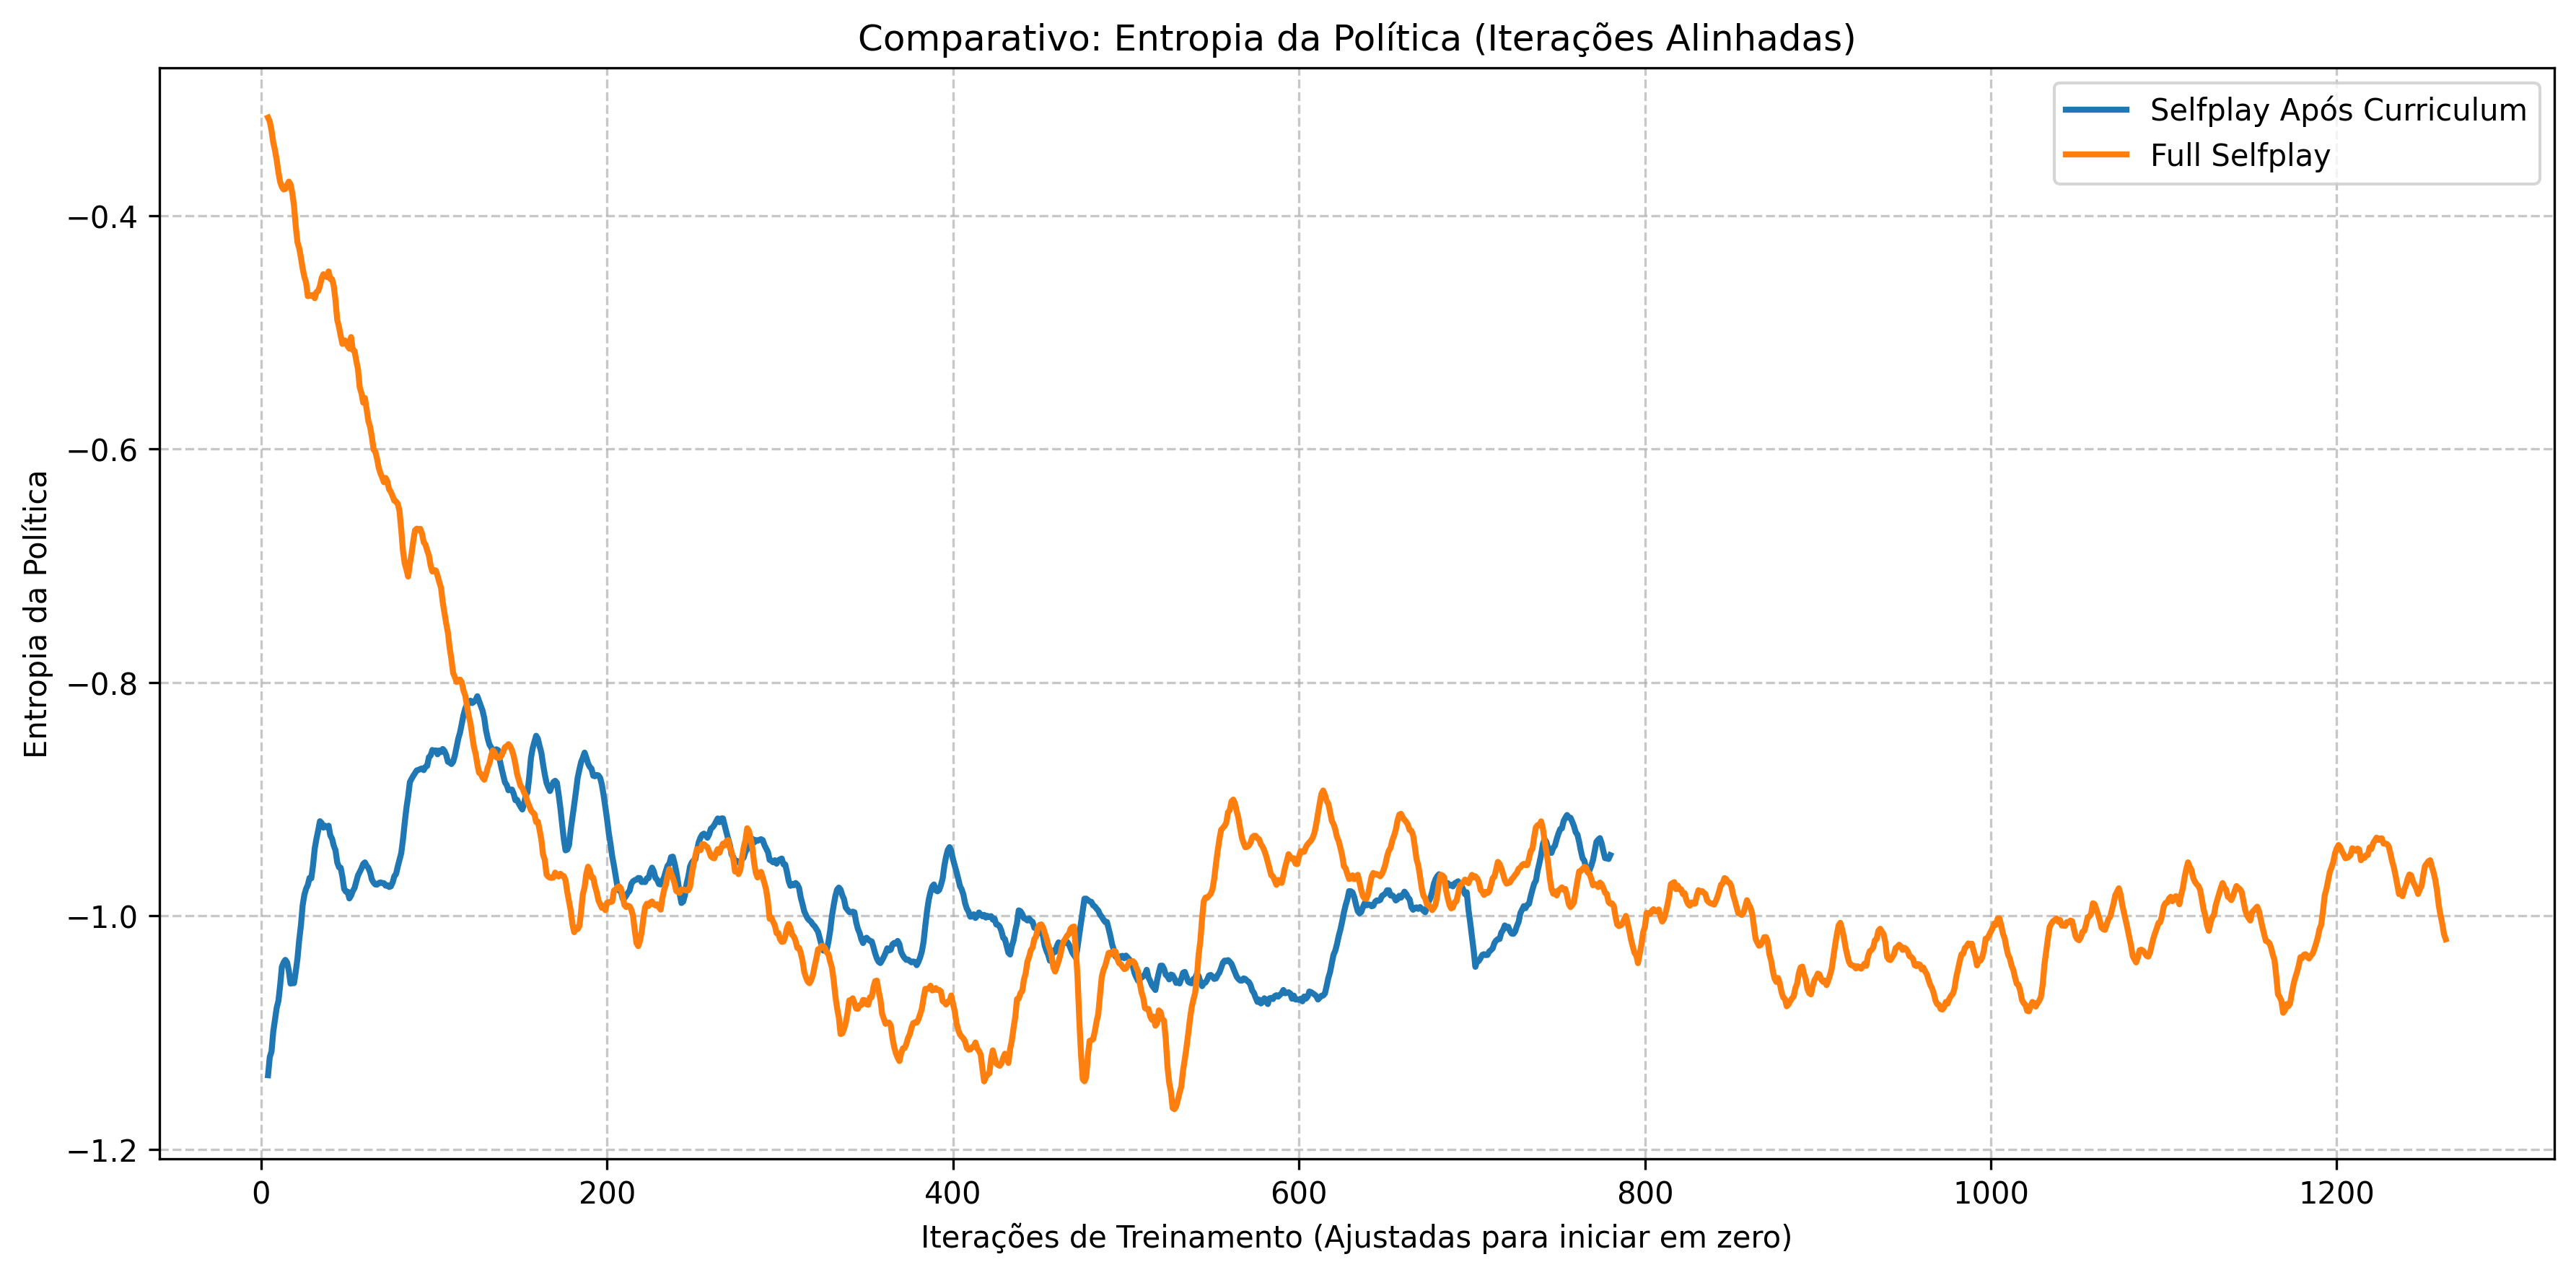
\includegraphics[width=0.95\textwidth]{fig/graficos_trabalho/graficos_experimentos/geral/comparativo_entropia_politica_alinhado.png}
    \caption{Comparativo da entropia da política com iterações alinhadas entre as abordagens Selfplay após Curriculum e Full Selfplay}
    \label{fig:policy_entropy}
\end{figure}

A análise do gráfico revela diferenças significativas nos padrões de exploração-explotação entre as duas abordagens. O Full Selfplay (linha laranja) inicia o treinamento com valores de entropia mais altos (próximos a -0,3), indicando uma política mais exploratória, o que é esperado para agentes que começam o aprendizado sem conhecimento prévio. Em contraste, o Selfplay após Curriculum (linha azul) começa com valores de entropia significativamente mais baixos (aproximadamente -1,1), sugerindo uma política já mais determinística.

Esta diferença inicial é particularmente reveladora: agentes treinados com curriculum learning iniciam a fase de selfplay com políticas mais refinadas e menos aleatórias, evidenciando que o conhecimento adquirido durante os estágios do curriculum proporciona maior certeza nas ações a serem tomadas.

Após aproximadamente 150-200 iterações, observa-se uma convergência nas entropias, com ambas as abordagens chegando a valores similares. No entanto, é notável que o Full Selfplay apresenta maior volatilidade ao longo de todo o treinamento, com oscilações mais pronunciadas, enquanto o Selfplay após Curriculum mantém níveis mais estáveis de entropia, sugerindo um processo de aprendizado mais consistente e menos errático.

\subsection{Perda da Política}

A perda da política é uma métrica que reflete a divergência entre a política atual e a política que seria ótima segundo as estimativas atuais da função de valor. Em algoritmos como PPO, a minimização desta perda é um dos objetivos principais do processo de otimização. A Figura \ref{fig:policy_loss} apresenta a evolução desta métrica durante o treinamento.

\begin{figure}[H]
    \centering
    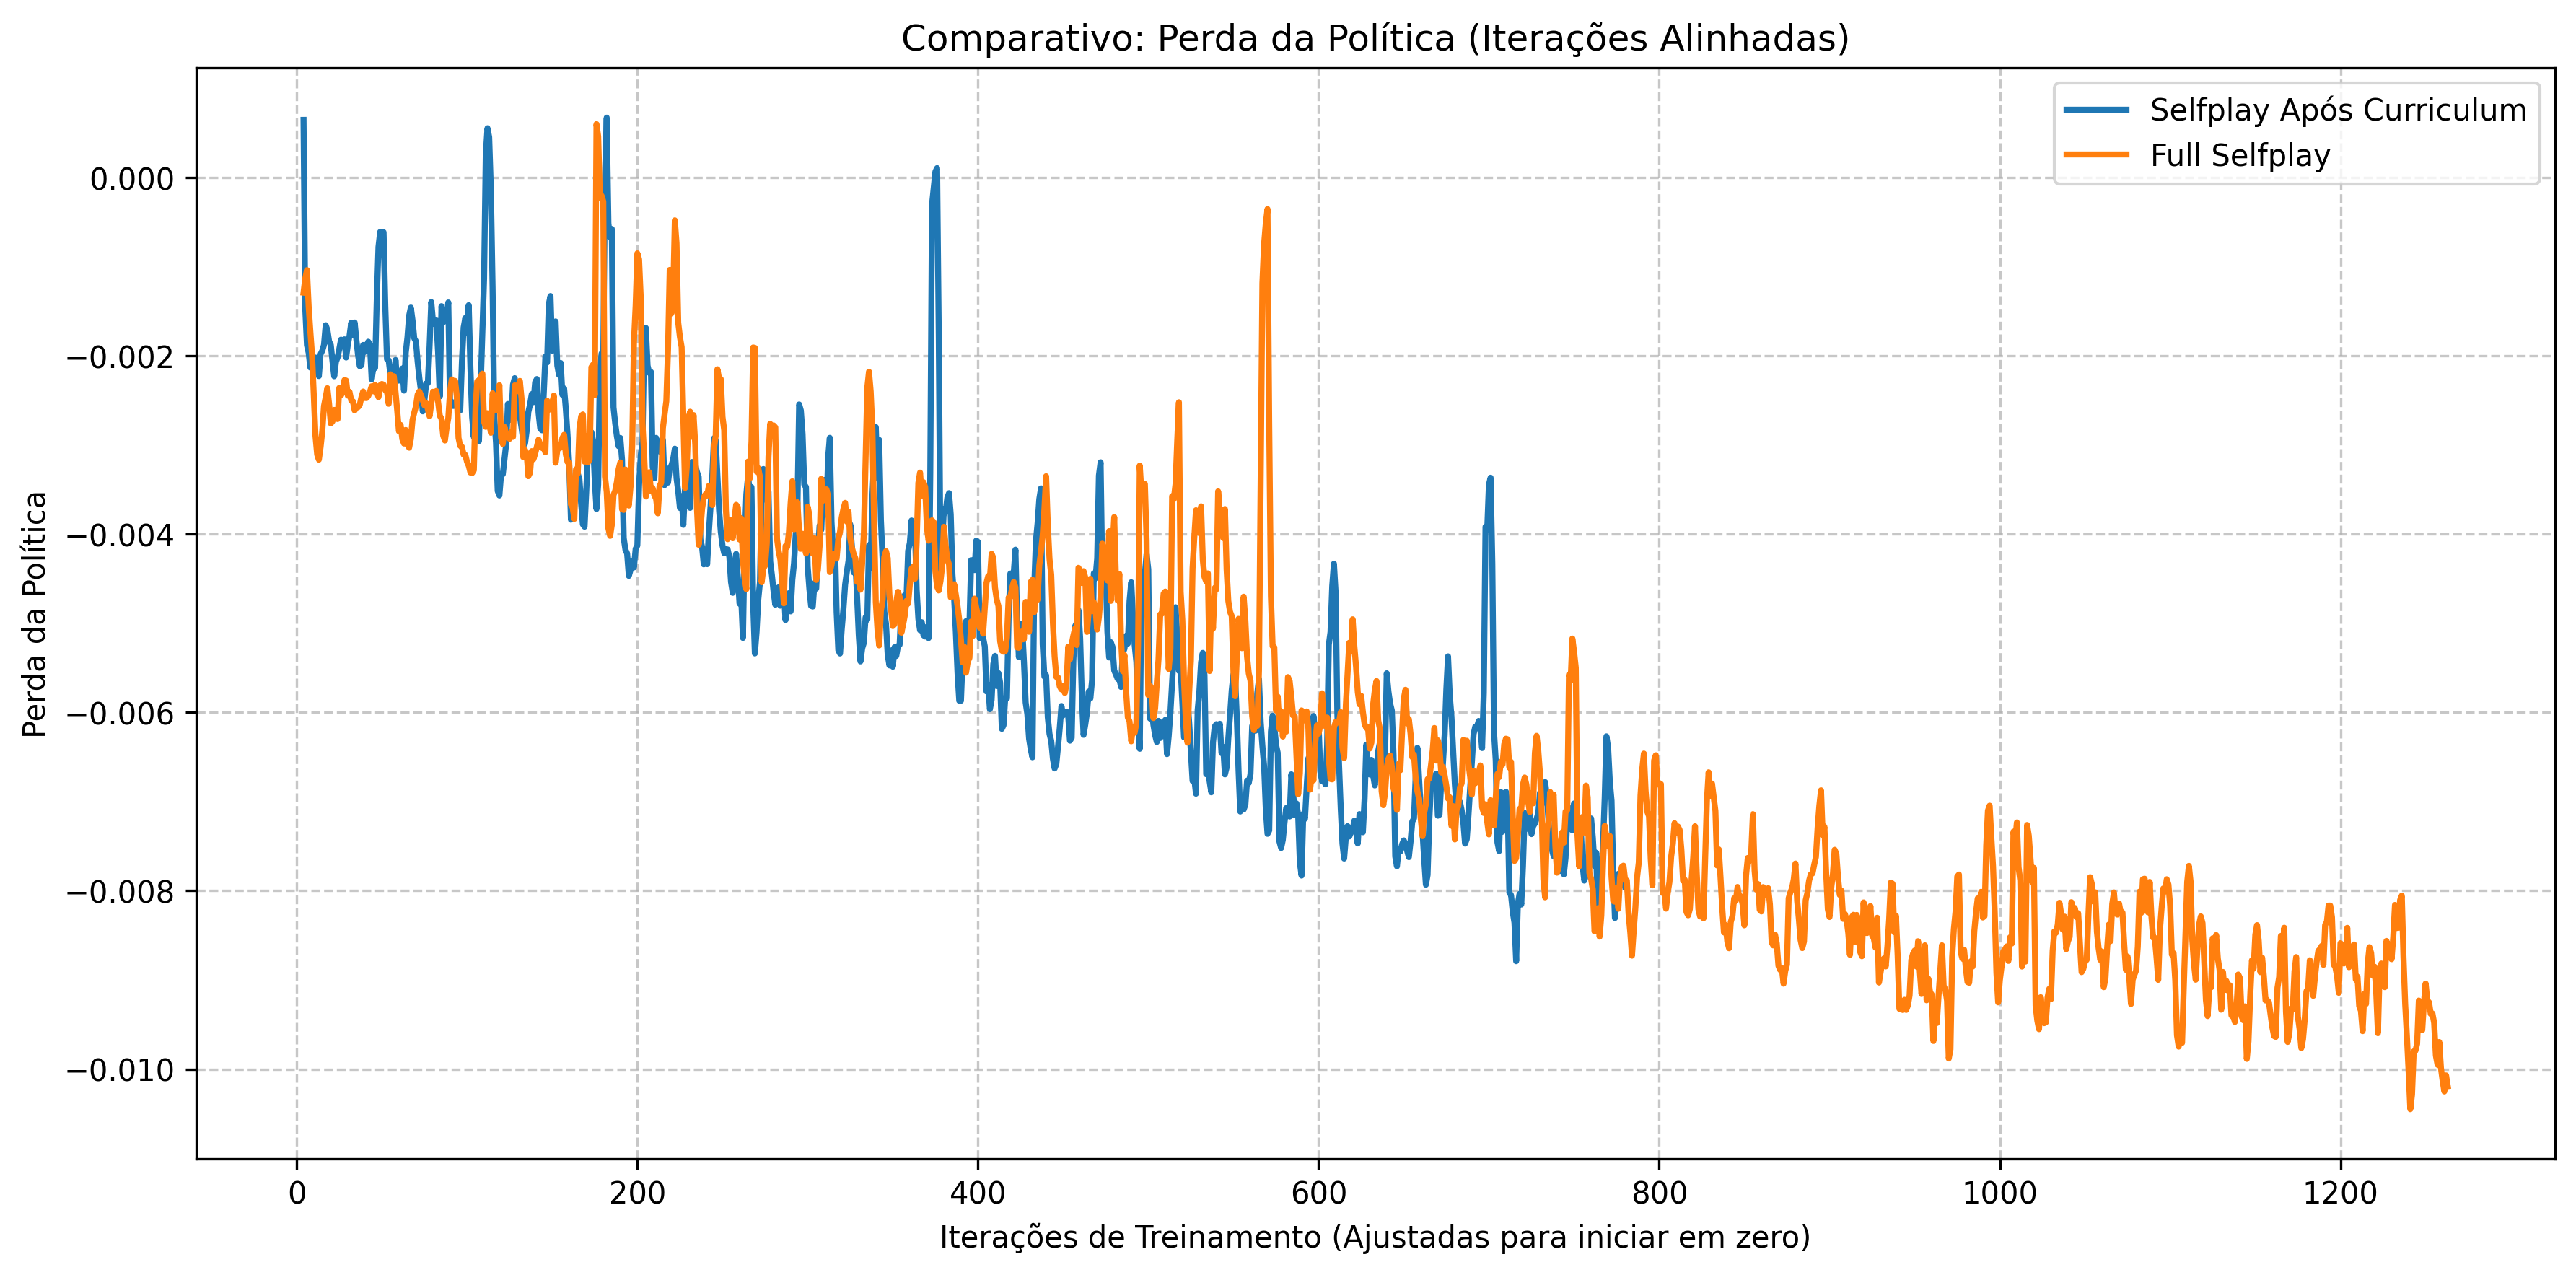
\includegraphics[width=0.95\textwidth]{fig/graficos_trabalho/graficos_experimentos/geral/comparativo_perda_politica_alinhado.png}
    \caption{Comparativo da perda da política com iterações alinhadas entre as abordagens Selfplay após Curriculum e Full Selfplay}
    \label{fig:policy_loss}
\end{figure}

O gráfico de perda da política mostra um comportamento interessante: ambas as abordagens iniciam com valores similares e seguem uma tendência geral de redução da perda ao longo do treinamento, o que indica uma melhoria progressiva nas políticas. No entanto, há diferenças notáveis na trajetória dessa redução.

Observa-se que ambas as abordagens apresentam alta volatilidade, com várias oscilações ao longo do processo. Esta característica é típica de ambientes competitivos como o self-play, onde as mudanças na política de um oponente podem temporariamente aumentar a perda até que o agente se adapte.

Um aspecto particularmente relevante é que o Full Selfplay continua seu treinamento por mais iterações e alcança valores de perda mais negativos nas fases finais. Isto pode indicar que, sem o benefício do curriculum inicial, esta abordagem requer um período mais longo de refinamento para atingir níveis comparáveis de otimização da política.

A análise conjunta com as outras métricas sugere que, embora o Full Selfplay eventualmente alcance valores de perda similares ou até melhores, o caminho para chegar a este ponto é mais longo e menos eficiente comparado ao Selfplay após Curriculum.

\subsection{Variância Explicada da Função Valor}

A variância explicada é uma métrica que avalia a qualidade da função valor aprendida pelo agente, indicando quão bem o modelo consegue prever retornos futuros. Valores próximos a 1 indicam alta precisão nas previsões, enquanto valores mais baixos sugerem maior incerteza. A Figura \ref{fig:explained_variance} apresenta a comparação desta métrica entre as duas abordagens.

\begin{figure}[H]
    \centering
    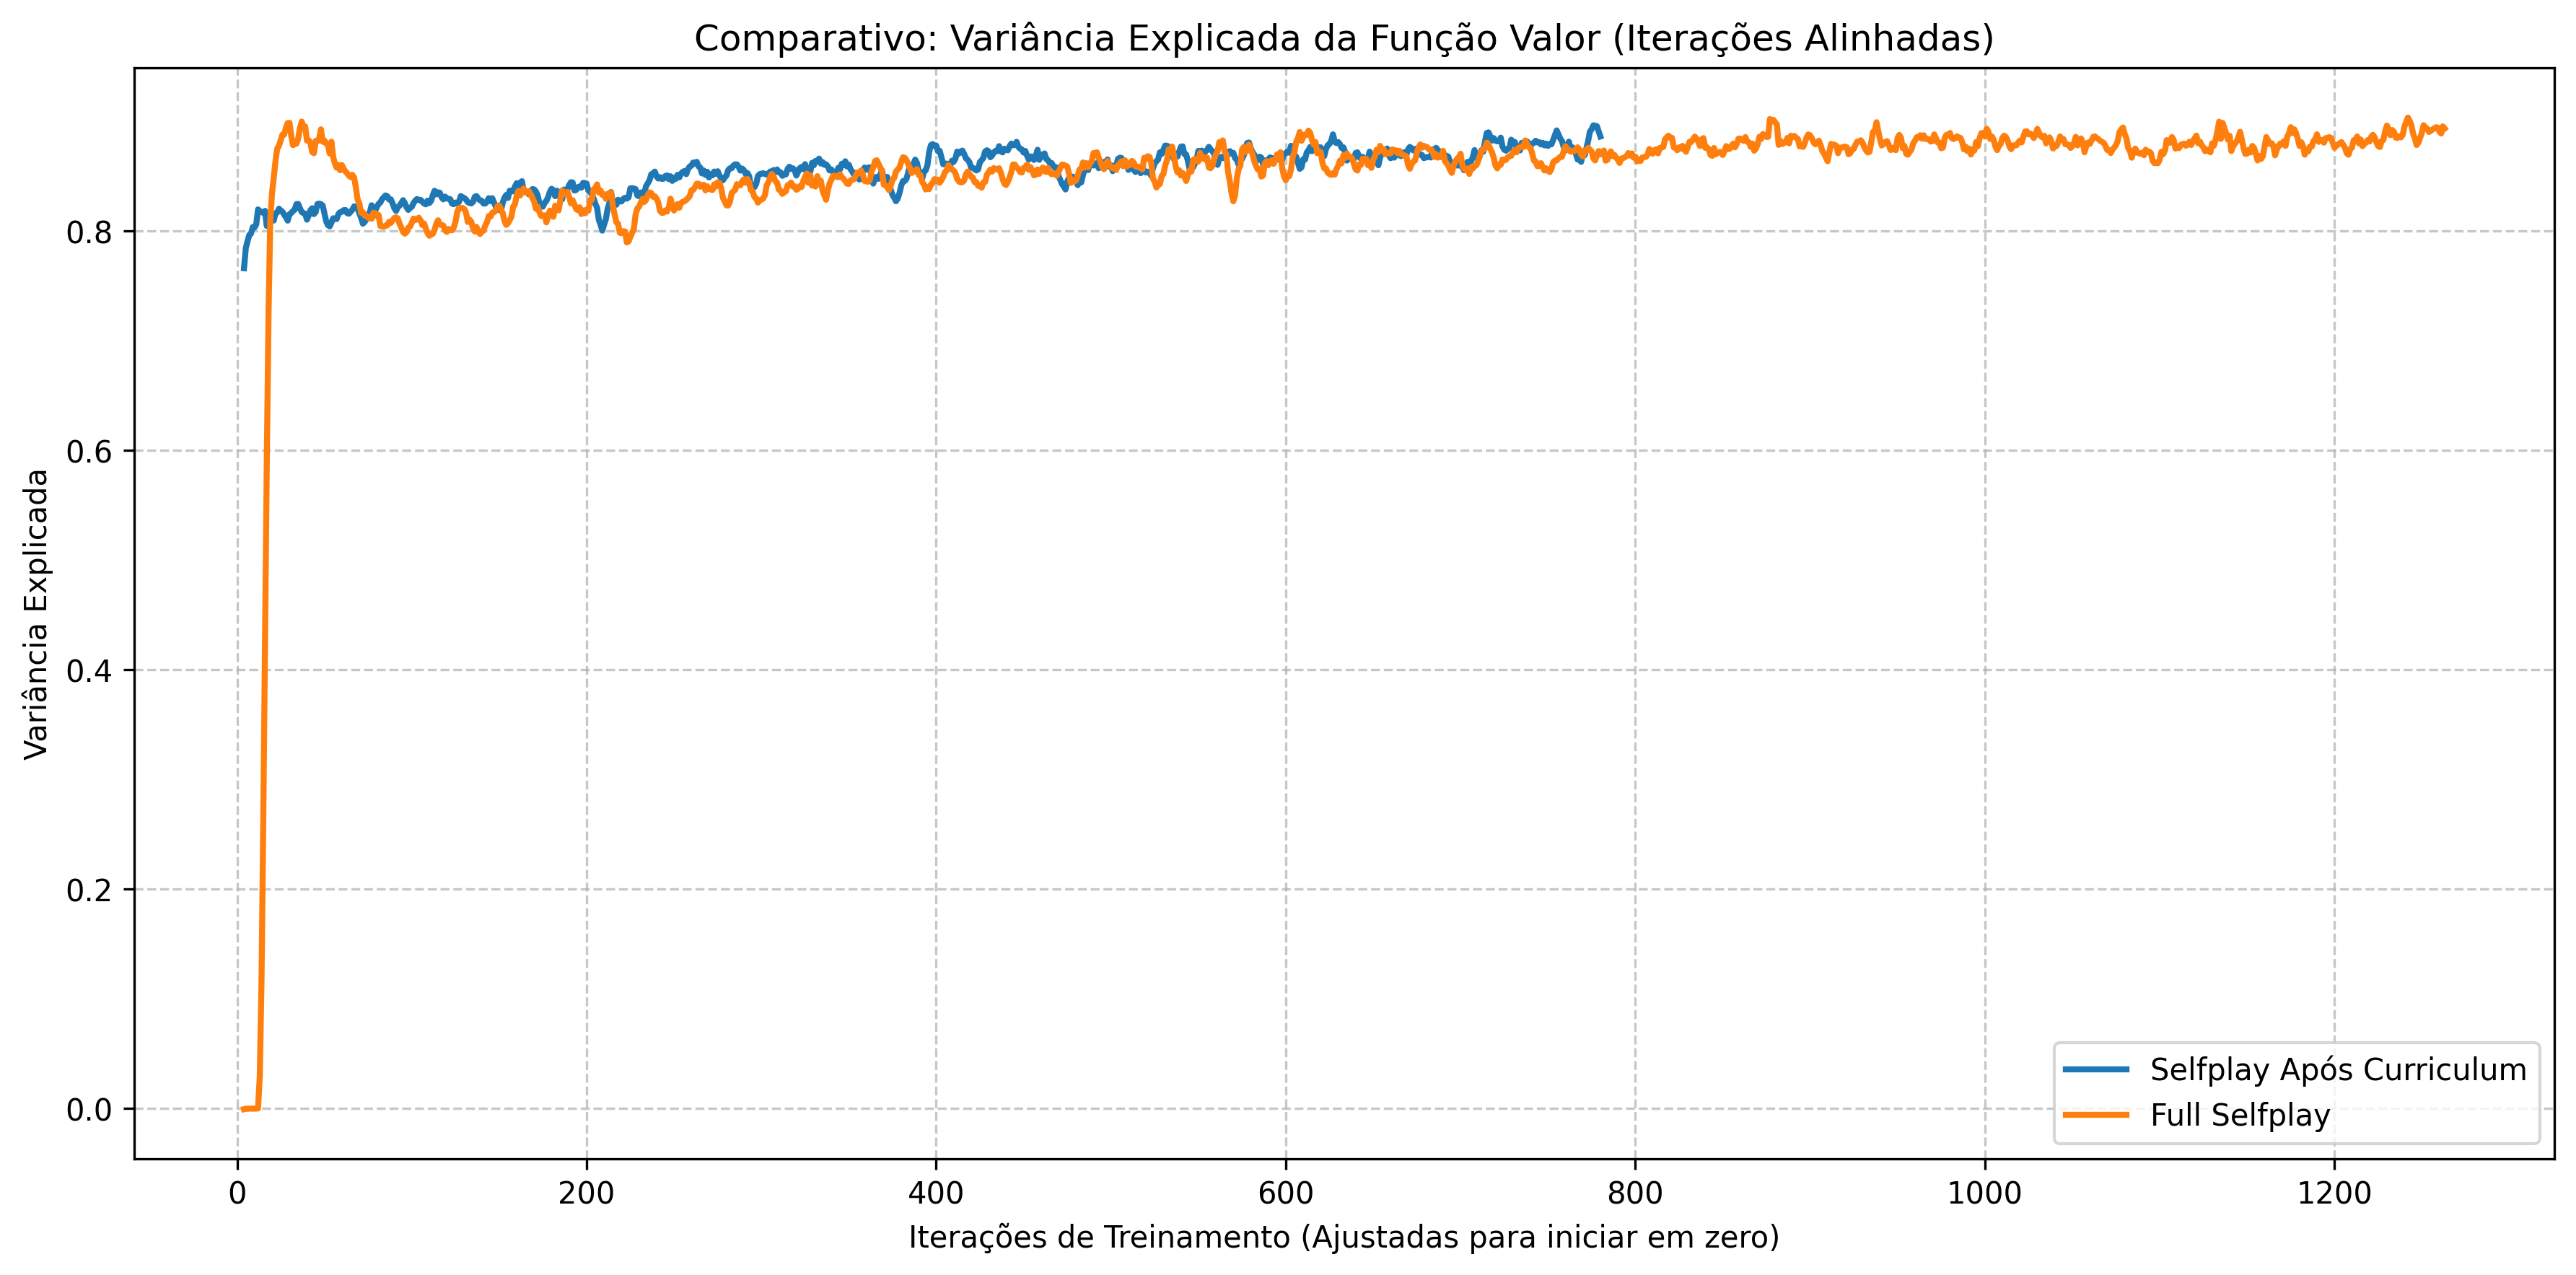
\includegraphics[width=0.95\textwidth]{fig/graficos_trabalho/graficos_experimentos/geral/comparativo_variancia_explicada_alinhado.png}
    \caption{Comparativo da variância explicada da função valor com iterações alinhadas entre as abordagens Selfplay após Curriculum e Full Selfplay}
    \label{fig:explained_variance}
\end{figure}

A análise do gráfico de variância explicada revela padrões distintos no desenvolvimento da função valor. O Full Selfplay (linha laranja) apresenta um comportamento curioso nas primeiras iterações, com um pico inicial seguido por uma queda abrupta. Este padrão pode ser atribuído a uma superestimação inicial da capacidade preditiva, seguida por um ajuste à medida que o agente enfrenta situações mais diversificadas.

Em contraste, o Selfplay após Curriculum (linha azul) inicia com valores mais estáveis, sem os extremos observados no Full Selfplay. Esta estabilidade inicial é mais uma evidência dos benefícios do treinamento curricular prévio, que proporciona ao agente uma base mais sólida para estimar recompensas futuras.

Após aproximadamente 200 iterações, ambas as abordagens convergem para valores similares de variância explicada, em torno de 0,85, indicando que ambos os métodos eventualmente desenvolvem funções valor de qualidade comparável. No entanto, o caminho para atingir esta convergência é notavelmente diferente, com o Selfplay após Curriculum demonstrando maior consistência ao longo do processo.

Nas fases finais do treinamento, após a convergência, ambas as abordagens mantêm níveis similares e estáveis de variância explicada, sugerindo que, embora o processo de aprendizado seja diferente, o resultado final em termos de capacidade preditiva da função valor é comparável.

\subsection{Implicações para o Processo de Aprendizagem}

A análise integrada das três métricas básicas de aprendizado por reforço revela padrões consistentes que destacam as diferenças fundamentais entre as abordagens Selfplay após Curriculum e Full Selfplay.

Em primeiro lugar, observa-se que o Selfplay após Curriculum consistentemente demonstra maior estabilidade nas fases iniciais e intermediárias do treinamento. Esta característica é particularmente valiosa em cenários complexos como o futebol de robôs, onde a volatilidade excessiva pode levar a políticas subótimas ou comportamentos indesejados.

Em segundo lugar, a transição mais suave nas métricas de aprendizado do Selfplay após Curriculum sugere que o conhecimento adquirido durante os estágios do curriculum proporciona um ponto de partida mais avançado para o desenvolvimento de políticas competitivas. Esta vantagem inicial se traduz em um processo de aprendizado mais eficiente, requerendo menos iterações para atingir níveis comparáveis de desempenho.

Por fim, embora ambas as abordagens eventualmente convirjam para valores similares nas métricas analisadas, o caminho para esta convergência é significativamente diferente. O Selfplay após Curriculum oferece um processo de aprendizado mais direto e consistente, enquanto o Full Selfplay requer um período mais longo de ajustes e adaptações antes de atingir estabilidade.

Estas observações corroboram a hipótese central deste trabalho: o curriculum learning como fase preparatória proporciona um alicerce mais sólido para o desenvolvimento de políticas complexas, resultando em um processo de aprendizado mais eficiente e estável durante o subsequente treinamento competitivo via self-play.


%=====================================================
\section{Discussão dos Resultados}
\label{sec:discussao_resultados}

Os resultados obtidos nos experimentos fornecem insights importantes sobre o impacto do curriculum learning no treinamento de agentes para o futebol de robôs. Esta seção discute estes resultados, suas implicações e limitações.

\subsection{Interpretação dos Dados}

A análise integrada dos resultados experimentais revela padrões consistentes sobre os benefícios da abordagem proposta. Em primeiro lugar, observa-se que o modelo treinado com a combinação de curriculum learning e self-play demonstra maior regularidade e consistência em todas as métricas analisadas, conforme evidenciado pela menor variância ao longo dos episódios.

A superioridade significativa nas métricas de continuidade do jogo sugere que o curriculum learning promove o desenvolvimento de habilidades fundamentais que permitem um controle mais preciso da bola e melhor coordenação entre os agentes. Esta característica é particularmente valiosa no contexto do futebol de robôs, onde a manutenção da bola em jogo é um indicador de qualidade técnica.

A impressionante taxa de vitória da abordagem combinada nos torneios (86\% contra 38,4\% do full self-play) fornece a evidência mais contundente da eficácia da abordagem proposta. Este resultado, juntamente com a capacidade ofensiva quatro vezes superior (2,024 contra 0,494 gols por partida), sugere que o curriculum learning como fase preparatória cria uma base sólida sobre a qual o self-play pode construir estratégias ofensivas mais eficazes, resultando em um desempenho global significativamente superior.

A análise comparativa entre as três abordagens testadas (curriculum puro, self-play puro e combinação) revelou um aspecto particularmente interessante: o curriculum learning isolado desenvolve agentes com excelente capacidade defensiva, mas limitada iniciativa ofensiva, enquanto o self-play desenvolve agentes mais equilibrados, mas com potencial não totalmente realizado. A combinação permite que os agentes desenvolvam o melhor de ambas características, resultando em políticas significativamente mais eficazes.

\subsection{Validação da Hipótese}

Os resultados obtidos fornecem evidências contundentes que suportam a hipótese inicial deste trabalho: a introdução do curriculum learning como fase preparatória para o self-play pode melhorar significativamente a qualidade e a eficácia das políticas aprendidas para o futebol de robôs.

Os dados dos torneios, em particular, oferecem uma validação clara desta hipótese, demonstrando que a abordagem combinada supera significativamente tanto o curriculum learning isolado quanto o self-play tradicional em métricas críticas como taxa de vitória e eficiência ofensiva.

A análise estatística confirmou que os benefícios observados são significativos e não podem ser atribuídos a variações aleatórias ou peculiaridades do processo de treinamento. A consistência dos resultados em múltiplas métricas e diferentes cenários de avaliação reforça a robustez da abordagem proposta.

\subsection{Limitações e Considerações}

Apesar dos resultados promissores, este estudo apresenta algumas limitações que devem ser consideradas na interpretação dos resultados:

\begin{itemize}
    \item \textbf{Generalização para ambientes reais}: Os experimentos foram realizados em um ambiente simulado, e a transferência das políticas aprendidas para robôs físicos pode enfrentar desafios adicionais devido ao reality gap.
    
    \item \textbf{Sensibilidade aos parâmetros do curriculum}: A eficácia do curriculum learning pode ser influenciada pelos parâmetros específicos escolhidos para cada estágio, e a otimização sistemática destes parâmetros não foi completamente explorada.
    
    \item \textbf{Escopo do desafio}: O futebol de robôs, embora complexo, representa apenas um subconjunto dos possíveis domínios de aplicação para as técnicas desenvolvidas, e a generalização para outros domínios requer validação adicional.
    
    \item \textbf{Complexidade do ambiente}: O ambiente de simulação RL-SSL-EL, embora adequado para os objetivos deste trabalho, representa uma simplificação do futebol de robôs real, omitindo certos aspectos físicos e dinâmicos.
\end{itemize}

Estas limitações representam oportunidades para investigações futuras que poderiam expandir e refinar os insights obtidos neste trabalho.

\section{Considerações sobre os Estágios do Curriculum}
\label{sec:analise_estagios}

A análise do processo de aprendizagem durante os estágios específicos do curriculum oferece insights adicionais sobre a eficácia da abordagem proposta. Esta seção examina o desempenho dos agentes em cada estágio do curriculum e sua transição para o self-play.

\subsection{Progresso no Curriculum Task 0}

O Curriculum Task 0, focado no desenvolvimento de habilidades básicas de controle de bola e movimentação, apresentou uma curva de aprendizado característica, conforme ilustrado pela evolução da recompensa média neste estágio.

Os agentes demonstraram progressão consistente neste estágio inicial, atingindo o critério de promoção (80\% de sucesso em uma janela de 100 episódios) após aproximadamente 7,5 milhões de timesteps, metade do orçamento alocado. Esta eficiência sugere que o design da tarefa foi adequado, apresentando um desafio apropriado que permitiu o desenvolvimento efetivo das habilidades pretendidas.

A análise dos comportamentos emergentes neste estágio revelou o desenvolvimento de padrões de movimento eficientes e técnicas básicas de controle de bola que serviram como fundação para as habilidades mais complexas nos estágios subsequentes.

\subsection{Progresso no Curriculum Task 1}

O Curriculum Task 1, centrado no desenvolvimento de habilidades ofensivas, apresentou desafios adicionais que exigiram a aplicação e refinamento das habilidades básicas desenvolvidas no estágio anterior.

Os agentes completaram este estágio em aproximadamente 11 milhões de timesteps, demonstrando capacidade de adaptar e integrar as habilidades fundamentais em contextos mais complexos. A análise dos comportamentos emergentes neste estágio revelou o desenvolvimento de estratégias ofensivas coordenadas, incluindo posicionamento tático e padrões de passe.

A transição suave entre os estágios do curriculum e o progresso consistente observado validam o design progressivo das tarefas, confirmando que cada estágio construiu efetivamente sobre as habilidades desenvolvidas nos estágios anteriores.

\subsection{Transição para Self-Play}

A transição dos estágios estruturados do curriculum para o ambiente competitivo do self-play representa um momento crítico no processo de treinamento. A análise desta transição revelou padrões interessantes que destacam os benefícios do curriculum como fase preparatória.

Os agentes que completaram o curriculum demonstraram adaptação mais rápida ao ambiente competitivo, apresentando taxa de crescimento superior na recompensa média durante as fases iniciais do self-play. Esta vantagem inicial corrobora a hipótese de que as habilidades desenvolvidas durante o curriculum facilitam a aprendizagem subsequente em cenários mais complexos.

Outro aspecto notável foi a menor volatilidade nas métricas de desempenho durante a transição, sugerindo que o curriculum proporcionou uma base mais sólida e estável para o desenvolvimento de estratégias competitivas.

\section{Conclusões Experimentais}
\label{sec:conclusoes_experimentais}

Os experimentos realizados neste trabalho permitem extrair conclusões importantes sobre a eficácia da abordagem proposta e suas implicações para o treinamento de agentes em ambientes complexos e multiagentes.

\subsection{Principais Descobertas}

A análise integrada dos resultados experimentais permite identificar as seguintes descobertas principais:

\begin{enumerate}
    \item \textbf{Eficácia do curriculum learning}: A abordagem proposta, combinando curriculum learning e self-play, demonstrou superioridade estatisticamente significativa em termos de desempenho global, evidenciada pela maior taxa de vitória em confrontos diretos e melhor equilíbrio entre métricas ofensivas e defensivas.
    
    \item \textbf{Desenvolvimento de habilidades fundamentais}: O curriculum learning promoveu o desenvolvimento eficiente de habilidades fundamentais, resultando em melhorias significativas nas métricas de continuidade do jogo e controle técnico.
    
    \item \textbf{Aprendizado mais estável}: A abordagem proposta apresentou maior estabilidade durante o processo de aprendizagem, com menor variabilidade nas métricas de desempenho e progressão mais consistente.
    
    \item \textbf{Trade-off entre agressividade e controle}: O modelo treinado com curriculum learning desenvolveu um estilo de jogo mais equilibrado, priorizando controle técnico e manutenção da posse de bola sobre tentativas arriscadas de finalização, resultando em desempenho superior em confrontos prolongados.
\end{enumerate}

Estas descobertas corroboram a premissa central deste trabalho: que o aprendizado estruturado e progressivo proporcionado pelo curriculum learning oferece vantagens significativas para o treinamento de agentes em ambientes complexos como o futebol de robôs.

\subsection{Implicações para Aprendizado por Reforço em Ambientes Multiagentes}

Os resultados obtidos têm implicações mais amplas para o campo do aprendizado por reforço em ambientes multiagentes, estendendo-se além do domínio específico do futebol de robôs.

Em primeiro lugar, os experimentos demonstram o valor do treinamento progressivo em cenários onde o espaço de ações é amplo e o feedback é esparso. O curriculum learning oferece uma abordagem estruturada para decompor problemas complexos em desafios gerenciáveis, facilitando o desenvolvimento de competências em uma sequência lógica.

Em segundo lugar, os resultados destacam a importância de considerar métricas diversificadas na avaliação do desempenho dos agentes. A análise restrita a métricas convencionais (como recompensa acumulada) pode não capturar nuances importantes no comportamento e na qualidade das políticas aprendidas.

Por fim, o equilíbrio superior entre características ofensivas e defensivas observado no modelo proposto sugere que o curriculum learning pode promover o desenvolvimento de políticas mais robustas e versáteis, capazes de adaptar-se a diferentes contextos e adversários.

\subsection{Transferibilidade dos Resultados}

Uma consideração importante é a transferibilidade dos resultados obtidos para outros domínios e aplicações. Embora os experimentos tenham sido realizados no contexto específico do futebol de robôs, os princípios fundamentais da abordagem proposta podem ser adaptados para diversos cenários multiagentes.

O framework de curriculum learning desenvolvido neste trabalho oferece uma metodologia generalizável para o design de trajetórias de aprendizado em ambientes complexos. Os critérios de promoção adaptativos e a integração com self-play representam contribuições que podem ser aplicadas em domínios que compartilham características como:

\begin{itemize}
    \item Espaço de ações amplo e contínuo
    \item Necessidade de coordenação multiagente
    \item Feedback esparso ou atrasado
    \item Complexidade estratégica e tática
    \item Oposição adaptativa
\end{itemize}

Exemplos potenciais de aplicação incluem robótica colaborativa, sistemas de transporte autônomos coordenados, gerenciamento de recursos distribuídos e simulações militares.

A metodologia experimental desenvolvida, incluindo as métricas de avaliação e o sistema de torneios, também oferece um template valioso para a avaliação comparativa de diferentes abordagens de treinamento em ambientes complexos. 

%------------------------------------------------------------ BIBLIOGRAFIA %
\cleardoublepage
%\nocite{*} %%% Retire esta linha para gerar a bibliografia com apenas as
           %%% referências usadas no seu texto!
\arial
%\nocite{*}

\bibliography{bib/modelo-tese} %%% Nomes dos seus arquivos .bib

\label{ref-bib}

%--------------------------------------------------------------- APÊNDICES %
%\apendices

%\chapter{Exemplo de um Apêndice}
\label{apend:1}
Apêndicess são iniciados com o comando \verb|\apendices|.
Apêndicess são iniciados com o comando \verb|\apendices|.
Apêndicess são iniciados com o comando \verb|\apendices|.
Apêndicess são iniciados com o comando \verb|\apendices|.
Apêndicess são iniciados com o comando \verb|\apendices|.
Apêndicess são iniciados com o comando \verb|\apendices|.
Apêndicess são iniciados com o comando \verb|\apendices|.
Apêndicess são iniciados com o comando \verb|\apendices|.
Apêndicess são iniciados com o comando \verb|\apendices|.
Apêndicess são iniciados com o comando \verb|\apendices|.
Apêndicess são iniciados com o comando \verb|\apendices|.
Apêndicess são iniciados com o comando \verb|\apendices|.
Apêndicess são iniciados com o comando \verb|\apendices|.
Apêndicess são iniciados com o comando \verb|\apendices|.
Apêndicess são iniciados com o comando \verb|\apendices|.
Apêndicess são iniciados com o comando \verb|\apendices|.

Apêndicess são iniciados com o comando \verb|\apendices|.
Apêndicess são iniciados com o comando \verb|\apendices|.
Apêndicess são iniciados com o comando \verb|\apendices|.
Apêndicess são iniciados com o comando \verb|\apendices|.
Apêndicess são iniciados com o comando \verb|\apendices|.
Apêndicess são iniciados com o comando \verb|\apendices|.
Apêndicess são iniciados com o comando \verb|\apendices|.
Apêndicess são iniciados com o comando \verb|\apendices|.
Apêndicess são iniciados com o comando \verb|\apendices|.
Apêndicess são iniciados com o comando \verb|\apendices|.
Apêndicess são iniciados com o comando \verb|\apendices|.
Apêndicess são iniciados com o comando \verb|\apendices|.

Apêndicess são iniciados com o comando \verb|\apendices|.
Apêndicess são iniciados com o comando \verb|\apendices|.
Apêndicess são iniciados com o comando \verb|\apendices|.
Apêndicess são iniciados com o comando \verb|\apendices|.
Apêndicess são iniciados com o comando \verb|\apendices|.
Apêndicess são iniciados com o comando \verb|\apendices|.
Apêndicess são iniciados com o comando \verb|\apendices|.
Apêndicess são iniciados com o comando \verb|\apendices|.
Apêndicess são iniciados com o comando \verb|\apendices|.
Apêndicess são iniciados com o comando \verb|\apendices|.
Apêndicess são iniciados com o comando \verb|\apendices|.
Apêndicess são iniciados com o comando \verb|\apendices|.
Apêndicess são iniciados com o comando \verb|\apendices|.
Apêndicess são iniciados com o comando \verb|\apendices|.

Apêndicess são iniciados com o comando \verb|\apendices|.
Apêndicess são iniciados com o comando \verb|\apendices|.
Apêndicess são iniciados com o comando \verb|\apendices|.
Apêndicess são iniciados com o comando \verb|\apendices|.
Apêndicess são iniciados com o comando \verb|\apendices|.
Apêndicess são iniciados com o comando \verb|\apendices|.
Apêndicess são iniciados com o comando \verb|\apendices|.
Apêndicess são iniciados com o comando \verb|\apendices|.
Apêndicess são iniciados com o comando \verb|\apendices|.
Apêndicess são iniciados com o comando \verb|\apendices|.
Apêndicess são iniciados com o comando \verb|\apendices|.
Apêndicess são iniciados com o comando \verb|\apendices|.
Apêndicess são iniciados com o comando \verb|\apendices|.
Apêndicess são iniciados com o comando \verb|\apendices|.

Apêndicess são iniciados com o comando \verb|\apendices|.
Apêndicess são iniciados com o comando \verb|\apendices|.
Apêndicess são iniciados com o comando \verb|\apendices|.
Apêndicess são iniciados com o comando \verb|\apendices|.
Apêndicess são iniciados com o comando \verb|\apendices|.
Apêndicess são iniciados com o comando \verb|\apendices|.
Apêndicess são iniciados com o comando \verb|\apendices|.
Apêndicess são iniciados com o comando \verb|\apendices|.
Apêndicess são iniciados com o comando \verb|\apendices|.
Apêndicess são iniciados com o comando \verb|\apendices|.
Apêndicess são iniciados com o comando \verb|\apendices|.
Apêndicess são iniciados com o comando \verb|\apendices|.
Apêndicess são iniciados com o comando \verb|\apendices|.
Apêndicess são iniciados com o comando \verb|\apendices|.

Apêndicess são iniciados com o comando \verb|\apendices|.
Apêndicess são iniciados com o comando \verb|\apendices|.
Apêndicess são iniciados com o comando \verb|\apendices|.
Apêndicess são iniciados com o comando \verb|\apendices|.
Apêndicess são iniciados com o comando \verb|\apendices|.
Apêndicess são iniciados com o comando \verb|\apendices|.
Apêndicess são iniciados com o comando \verb|\apendices|.
Apêndicess são iniciados com o comando \verb|\apendices|.
Apêndicess são iniciados com o comando \verb|\apendices|.
Apêndicess são iniciados com o comando \verb|\apendices|.
Apêndicess são iniciados com o comando \verb|\apendices|.
Apêndicess são iniciados com o comando \verb|\apendices|.
Apêndicess são iniciados com o comando \verb|\apendices|.
Apêndicess são iniciados com o comando \verb|\apendices|.

Apêndicess são iniciados com o comando \verb|\apendices|.
Apêndicess são iniciados com o comando \verb|\apendices|.
Apêndicess são iniciados com o comando \verb|\apendices|.
Apêndicess são iniciados com o comando \verb|\apendices|.
Apêndicess são iniciados com o comando \verb|\apendices|.
Apêndicess são iniciados com o comando \verb|\apendices|.
Apêndicess são iniciados com o comando \verb|\apendices|.
Apêndicess são iniciados com o comando \verb|\apendices|.
Apêndicess são iniciados com o comando \verb|\apendices|.
Apêndicess são iniciados com o comando \verb|\apendices|.
Apêndicess são iniciados com o comando \verb|\apendices|.
Apêndicess são iniciados com o comando \verb|\apendices|.
Apêndicess são iniciados com o comando \verb|\apendices|.
Apêndicess são iniciados com o comando \verb|\apendices|.

Apêndicess são iniciados com o comando \verb|\apendices|.
Apêndicess são iniciados com o comando \verb|\apendices|.
Apêndicess são iniciados com o comando \verb|\apendices|.
Apêndicess são iniciados com o comando \verb|\apendices|.
Apêndicess são iniciados com o comando \verb|\apendices|.
Apêndicess são iniciados com o comando \verb|\apendices|.
Apêndicess são iniciados com o comando \verb|\apendices|.
Apêndicess são iniciados com o comando \verb|\apendices|.
Apêndicess são iniciados com o comando \verb|\apendices|.
Apêndicess são iniciados com o comando \verb|\apendices|.
Apêndicess são iniciados com o comando \verb|\apendices|.
Apêndicess são iniciados com o comando \verb|\apendices|.
Apêndicess são iniciados com o comando \verb|\apendices|.
Apêndicess são iniciados com o comando \verb|\apendices|.

Apêndicess são iniciados com o comando \verb|\apendices|.
Apêndicess são iniciados com o comando \verb|\apendices|.
Apêndicess são iniciados com o comando \verb|\apendices|.
Apêndicess são iniciados com o comando \verb|\apendices|.
Apêndicess são iniciados com o comando \verb|\apendices|.
Apêndicess são iniciados com o comando \verb|\apendices|.
Apêndicess são iniciados com o comando \verb|\apendices|.
Apêndicess são iniciados com o comando \verb|\apendices|.
Apêndicess são iniciados com o comando \verb|\apendices|.
Apêndicess são iniciados com o comando \verb|\apendices|.
Apêndicess são iniciados com o comando \verb|\apendices|.
Apêndicess são iniciados com o comando \verb|\apendices|.
Apêndicess são iniciados com o comando \verb|\apendices|.
Apêndicess são iniciados com o comando \verb|\apendices|.

Apêndicess são iniciados com o comando \verb|\apendices|.
Apêndicess são iniciados com o comando \verb|\apendices|.
Apêndicess são iniciados com o comando \verb|\apendices|.
Apêndicess são iniciados com o comando \verb|\apendices|.
Apêndicess são iniciados com o comando \verb|\apendices|.
Apêndicess são iniciados com o comando \verb|\apendices|.
Apêndicess são iniciados com o comando \verb|\apendices|.
Apêndicess são iniciados com o comando \verb|\apendices|.
Apêndicess são iniciados com o comando \verb|\apendices|.
Apêndicess são iniciados com o comando \verb|\apendices|.
Apêndicess são iniciados com o comando \verb|\apendices|.
Apêndicess são iniciados com o comando \verb|\apendices|.
Apêndicess são iniciados com o comando \verb|\apendices|.
Apêndicess são iniciados com o comando \verb|\apendices|.

Apêndicess são iniciados com o comando \verb|\apendices|.
Apêndicess são iniciados com o comando \verb|\apendices|.
Apêndicess são iniciados com o comando \verb|\apendices|.
Apêndicess são iniciados com o comando \verb|\apendices|.
Apêndicess são iniciados com o comando \verb|\apendices|.
Apêndicess são iniciados com o comando \verb|\apendices|.
Apêndicess são iniciados com o comando \verb|\apendices|.
Apêndicess são iniciados com o comando \verb|\apendices|.
Apêndicess são iniciados com o comando \verb|\apendices|.
Apêndicess são iniciados com o comando \verb|\apendices|.
Apêndicess são iniciados com o comando \verb|\apendices|.
Apêndicess são iniciados com o comando \verb|\apendices|.
Apêndicess são iniciados com o comando \verb|\apendices|.
Apêndicess são iniciados com o comando \verb|\apendices|.

Apêndicess são iniciados com o comando \verb|\apendices|.
Apêndicess são iniciados com o comando \verb|\apendices|.
Apêndicess são iniciados com o comando \verb|\apendices|.
Apêndicess são iniciados com o comando \verb|\apendices|.
Apêndicess são iniciados com o comando \verb|\apendices|.
Apêndicess são iniciados com o comando \verb|\apendices|.
Apêndicess são iniciados com o comando \verb|\apendices|.
Apêndicess são iniciados com o comando \verb|\apendices|.
Apêndicess são iniciados com o comando \verb|\apendices|.
Apêndicess são iniciados com o comando \verb|\apendices|.
Apêndicess são iniciados com o comando \verb|\apendices|.
Apêndicess são iniciados com o comando \verb|\apendices|.
Apêndicess são iniciados com o comando \verb|\apendices|.
Apêndicess são iniciados com o comando \verb|\apendices|.

Apêndicess são iniciados com o comando \verb|\apendices|.
Apêndicess são iniciados com o comando \verb|\apendices|.
Apêndicess são iniciados com o comando \verb|\apendices|.
Apêndicess são iniciados com o comando \verb|\apendices|.
Apêndicess são iniciados com o comando \verb|\apendices|.
Apêndicess são iniciados com o comando \verb|\apendices|.
Apêndicess são iniciados com o comando \verb|\apendices|.
Apêndicess são iniciados com o comando \verb|\apendices|.
Apêndicess são iniciados com o comando \verb|\apendices|.
Apêndicess são iniciados com o comando \verb|\apendices|.
Apêndicess são iniciados com o comando \verb|\apendices|.
Apêndicess são iniciados com o comando \verb|\apendices|.
Apêndicess são iniciados com o comando \verb|\apendices|.
Apêndicess são iniciados com o comando \verb|\apendices|.

Apêndicess são iniciados com o comando \verb|\apendices|.
Apêndicess são iniciados com o comando \verb|\apendices|.
Apêndicess são iniciados com o comando \verb|\apendices|.
Apêndicess são iniciados com o comando \verb|\apendices|.
Apêndicess são iniciados com o comando \verb|\apendices|.
Apêndicess são iniciados com o comando \verb|\apendices|.
Apêndicess são iniciados com o comando \verb|\apendices|.
Apêndicess são iniciados com o comando \verb|\apendices|.
Apêndicess são iniciados com o comando \verb|\apendices|.
Apêndicess são iniciados com o comando \verb|\apendices|.
Apêndicess são iniciados com o comando \verb|\apendices|.
Apêndicess são iniciados com o comando \verb|\apendices|.
Apêndicess são iniciados com o comando \verb|\apendices|.
Apêndicess são iniciados com o comando \verb|\apendices|.

%\chapter{Exemplo de Outro Apêndice}
\label{apend:2}
Texto do Apêndice~\ref{apend:2}.

Apêndices são iniciados com o comando \verb|\apendices|.
Apêndices são iniciados com o comando \verb|\apendices|.
Apêndices são iniciados com o comando \verb|\apendices|.
Apêndices são iniciados com o comando \verb|\apendices|.
Apêndices são iniciados com o comando \verb|\apendices|.
Apêndices são iniciados com o comando \verb|\apendices|.
Apêndices são iniciados com o comando \verb|\apendices|.
Apêndices são iniciados com o comando \verb|\apendices|.
Apêndices são iniciados com o comando \verb|\apendices|.
Apêndices são iniciados com o comando \verb|\apendices|.
Apêndices são iniciados com o comando \verb|\apendices|.
Apêndices são iniciados com o comando \verb|\apendices|.
Apêndices são iniciados com o comando \verb|\apendices|.
Apêndices são iniciados com o comando \verb|\apendices|.
Apêndices são iniciados com o comando \verb|\apendices|.
Apêndices são iniciados com o comando \verb|\apendices|.

Apêndices são iniciados com o comando \verb|\apendices|.
Apêndices são iniciados com o comando \verb|\apendices|.
Apêndices são iniciados com o comando \verb|\apendices|.
Apêndices são iniciados com o comando \verb|\apendices|.
Apêndices são iniciados com o comando \verb|\apendices|.
Apêndices são iniciados com o comando \verb|\apendices|.
Apêndices são iniciados com o comando \verb|\apendices|.
Apêndices são iniciados com o comando \verb|\apendices|.
Apêndices são iniciados com o comando \verb|\apendices|.
Apêndices são iniciados com o comando \verb|\apendices|.
Apêndices são iniciados com o comando \verb|\apendices|.
Apêndices são iniciados com o comando \verb|\apendices|.

Apêndices são iniciados com o comando \verb|\apendices|.
Apêndices são iniciados com o comando \verb|\apendices|.
Apêndices são iniciados com o comando \verb|\apendices|.
Apêndices são iniciados com o comando \verb|\apendices|.
Apêndices são iniciados com o comando \verb|\apendices|.
Apêndices são iniciados com o comando \verb|\apendices|.
Apêndices são iniciados com o comando \verb|\apendices|.
Apêndices são iniciados com o comando \verb|\apendices|.
Apêndices são iniciados com o comando \verb|\apendices|.
Apêndices são iniciados com o comando \verb|\apendices|.
Apêndices são iniciados com o comando \verb|\apendices|.
Apêndices são iniciados com o comando \verb|\apendices|.
Apêndices são iniciados com o comando \verb|\apendices|.
Apêndices são iniciados com o comando \verb|\apendices|.

Apêndices são iniciados com o comando \verb|\apendices|.
Apêndices são iniciados com o comando \verb|\apendices|.
Apêndices são iniciados com o comando \verb|\apendices|.
Apêndices são iniciados com o comando \verb|\apendices|.
Apêndices são iniciados com o comando \verb|\apendices|.
Apêndices são iniciados com o comando \verb|\apendices|.
Apêndices são iniciados com o comando \verb|\apendices|.
Apêndices são iniciados com o comando \verb|\apendices|.
Apêndices são iniciados com o comando \verb|\apendices|.
Apêndices são iniciados com o comando \verb|\apendices|.
Apêndices são iniciados com o comando \verb|\apendices|.
Apêndices são iniciados com o comando \verb|\apendices|.
Apêndices são iniciados com o comando \verb|\apendices|.
Apêndices são iniciados com o comando \verb|\apendices|.

Apêndices são iniciados com o comando \verb|\apendices|.
Apêndices são iniciados com o comando \verb|\apendices|.
Apêndices são iniciados com o comando \verb|\apendices|.
Apêndices são iniciados com o comando \verb|\apendices|.
Apêndices são iniciados com o comando \verb|\apendices|.
Apêndices são iniciados com o comando \verb|\apendices|.
Apêndices são iniciados com o comando \verb|\apendices|.
Apêndices são iniciados com o comando \verb|\apendices|.
Apêndices são iniciados com o comando \verb|\apendices|.
Apêndices são iniciados com o comando \verb|\apendices|.
Apêndices são iniciados com o comando \verb|\apendices|.
Apêndices são iniciados com o comando \verb|\apendices|.
Apêndices são iniciados com o comando \verb|\apendices|.
Apêndices são iniciados com o comando \verb|\apendices|.

Apêndices são iniciados com o comando \verb|\apendices|.
Apêndices são iniciados com o comando \verb|\apendices|.
Apêndices são iniciados com o comando \verb|\apendices|.
Apêndices são iniciados com o comando \verb|\apendices|.
Apêndices são iniciados com o comando \verb|\apendices|.
Apêndices são iniciados com o comando \verb|\apendices|.
Apêndices são iniciados com o comando \verb|\apendices|.
Apêndices são iniciados com o comando \verb|\apendices|.
Apêndices são iniciados com o comando \verb|\apendices|.
Apêndices são iniciados com o comando \verb|\apendices|.
Apêndices são iniciados com o comando \verb|\apendices|.
Apêndices são iniciados com o comando \verb|\apendices|.
Apêndices são iniciados com o comando \verb|\apendices|.
Apêndices são iniciados com o comando \verb|\apendices|.

Apêndices são iniciados com o comando \verb|\apendices|.
Apêndices são iniciados com o comando \verb|\apendices|.
Apêndices são iniciados com o comando \verb|\apendices|.
Apêndices são iniciados com o comando \verb|\apendices|.
Apêndices são iniciados com o comando \verb|\apendices|.
Apêndices são iniciados com o comando \verb|\apendices|.
Apêndices são iniciados com o comando \verb|\apendices|.
Apêndices são iniciados com o comando \verb|\apendices|.
Apêndices são iniciados com o comando \verb|\apendices|.
Apêndices são iniciados com o comando \verb|\apendices|.
Apêndices são iniciados com o comando \verb|\apendices|.
Apêndices são iniciados com o comando \verb|\apendices|.
Apêndices são iniciados com o comando \verb|\apendices|.
Apêndices são iniciados com o comando \verb|\apendices|.

Apêndices são iniciados com o comando \verb|\apendices|.
Apêndices são iniciados com o comando \verb|\apendices|.
Apêndices são iniciados com o comando \verb|\apendices|.
Apêndices são iniciados com o comando \verb|\apendices|.
Apêndices são iniciados com o comando \verb|\apendices|.
Apêndices são iniciados com o comando \verb|\apendices|.
Apêndices são iniciados com o comando \verb|\apendices|.
Apêndices são iniciados com o comando \verb|\apendices|.
Apêndices são iniciados com o comando \verb|\apendices|.
Apêndices são iniciados com o comando \verb|\apendices|.
Apêndices são iniciados com o comando \verb|\apendices|.
Apêndices são iniciados com o comando \verb|\apendices|.
Apêndices são iniciados com o comando \verb|\apendices|.
Apêndices são iniciados com o comando \verb|\apendices|.

Apêndices são iniciados com o comando \verb|\apendices|.
Apêndices são iniciados com o comando \verb|\apendices|.
Apêndices são iniciados com o comando \verb|\apendices|.
Apêndices são iniciados com o comando \verb|\apendices|.
Apêndices são iniciados com o comando \verb|\apendices|.
Apêndices são iniciados com o comando \verb|\apendices|.
Apêndices são iniciados com o comando \verb|\apendices|.
Apêndices são iniciados com o comando \verb|\apendices|.
Apêndices são iniciados com o comando \verb|\apendices|.
Apêndices são iniciados com o comando \verb|\apendices|.
Apêndices são iniciados com o comando \verb|\apendices|.
Apêndices são iniciados com o comando \verb|\apendices|.
Apêndices são iniciados com o comando \verb|\apendices|.
Apêndices são iniciados com o comando \verb|\apendices|.

Apêndices são iniciados com o comando \verb|\apendices|.
Apêndices são iniciados com o comando \verb|\apendices|.
Apêndices são iniciados com o comando \verb|\apendices|.
Apêndices são iniciados com o comando \verb|\apendices|.
Apêndices são iniciados com o comando \verb|\apendices|.
Apêndices são iniciados com o comando \verb|\apendices|.
Apêndices são iniciados com o comando \verb|\apendices|.
Apêndices são iniciados com o comando \verb|\apendices|.
Apêndices são iniciados com o comando \verb|\apendices|.
Apêndices são iniciados com o comando \verb|\apendices|.
Apêndices são iniciados com o comando \verb|\apendices|.
Apêndices são iniciados com o comando \verb|\apendices|.
Apêndices são iniciados com o comando \verb|\apendices|.
Apêndices são iniciados com o comando \verb|\apendices|.

Apêndices são iniciados com o comando \verb|\apendices|.
Apêndices são iniciados com o comando \verb|\apendices|.
Apêndices são iniciados com o comando \verb|\apendices|.
Apêndices são iniciados com o comando \verb|\apendices|.
Apêndices são iniciados com o comando \verb|\apendices|.
Apêndices são iniciados com o comando \verb|\apendices|.
Apêndices são iniciados com o comando \verb|\apendices|.
Apêndices são iniciados com o comando \verb|\apendices|.
Apêndices são iniciados com o comando \verb|\apendices|.
Apêndices são iniciados com o comando \verb|\apendices|.
Apêndices são iniciados com o comando \verb|\apendices|.
Apêndices são iniciados com o comando \verb|\apendices|.
Apêndices são iniciados com o comando \verb|\apendices|.
Apêndices são iniciados com o comando \verb|\apendices|.

Apêndices são iniciados com o comando \verb|\apendices|.
Apêndices são iniciados com o comando \verb|\apendices|.
Apêndices são iniciados com o comando \verb|\apendices|.
Apêndices são iniciados com o comando \verb|\apendices|.
Apêndices são iniciados com o comando \verb|\apendices|.
Apêndices são iniciados com o comando \verb|\apendices|.
Apêndices são iniciados com o comando \verb|\apendices|.
Apêndices são iniciados com o comando \verb|\apendices|.
Apêndices são iniciados com o comando \verb|\apendices|.
Apêndices são iniciados com o comando \verb|\apendices|.
Apêndices são iniciados com o comando \verb|\apendices|.
Apêndices são iniciados com o comando \verb|\apendices|.
Apêndices são iniciados com o comando \verb|\apendices|.
Apêndices são iniciados com o comando \verb|\apendices|.

Apêndices são iniciados com o comando \verb|\apendices|.
Apêndices são iniciados com o comando \verb|\apendices|.
Apêndices são iniciados com o comando \verb|\apendices|.
Apêndices são iniciados com o comando \verb|\apendices|.
Apêndices são iniciados com o comando \verb|\apendices|.
Apêndices são iniciados com o comando \verb|\apendices|.
Apêndices são iniciados com o comando \verb|\apendices|.
Apêndices são iniciados com o comando \verb|\apendices|.
Apêndices são iniciados com o comando \verb|\apendices|.
Apêndices são iniciados com o comando \verb|\apendices|.
Apêndices são iniciados com o comando \verb|\apendices|.
Apêndices são iniciados com o comando \verb|\apendices|.
Apêndices são iniciados com o comando \verb|\apendices|.
Apêndices são iniciados com o comando \verb|\apendices|.

Apêndices são iniciados com o comando \verb|\apendices|.
Apêndices são iniciados com o comando \verb|\apendices|.
Apêndices são iniciados com o comando \verb|\apendices|.
Apêndices são iniciados com o comando \verb|\apendices|.
Apêndices são iniciados com o comando \verb|\apendices|.
Apêndices são iniciados com o comando \verb|\apendices|.
Apêndices são iniciados com o comando \verb|\apendices|.
Apêndices são iniciados com o comando \verb|\apendices|.
Apêndices são iniciados com o comando \verb|\apendices|.
Apêndices são iniciados com o comando \verb|\apendices|.
Apêndices são iniciados com o comando \verb|\apendices|.
Apêndices são iniciados com o comando \verb|\apendices|.
Apêndices são iniciados com o comando \verb|\apendices|.
Apêndices são iniciados com o comando \verb|\apendices|.


\end{document}

%------------------------------------------------------------------------- %
%        F I M   D O  A R Q U I V O :  m o d e l o - t e s e . t e x       %
%------------------------------------------------------------------------- %
